\documentclass{rs}
\usepackage{amsmath,amssymb,amsthm,stmaryrd}
\usepackage[all]{xy}
\usepackage[usenames,dvipsnames]{xcolor}
\usepackage{tikz}
\usepackage{url}
\usepackage{hyperref}
\usepackage{enumerate}
\usepackage{tensor}
%/home/grad/zyf/TeX/inputs/
\usepackage{mathrsfs}
\usepackage{graphicx}
\usepackage{mathtools}
\usetikzlibrary{arrows}
%\usepackage{amsrefs}
%\usepackage{setspace}
%\doublespacing

%\title{Elliptic curves}
%\author{Yifei Zhu}
%\givenname{Yifei}
%\surname{Zhu}
%\address{Department of Mathematics\\University of Minnesota\\Minneapolis, MN 55455\\USA}
%\email{zyf@math.umn.edu}

%\subject{primary}{msc2000}{55P99}
%\subject{secondary}{msc2000}{55Q99}

%\bibliographystyle{gtart}
\parskip 0.7pc
\parindent 0pt

\newtheorem{thm}{Theorem}
\newtheorem{cor}[thm]{Corollary}
\newtheorem{prop}[thm]{Proposition}
\newtheorem{lem}[thm]{Lemma}
\theoremstyle{definition}
\newtheorem{defn}[thm]{Definition}
\theoremstyle{remark}
\newtheorem{rmk}[thm]{Remark}
\newtheorem{ex}[thm]{Example}
\newtheorem{case}[thm]{Case}
\newtheorem{slogan}[thm]{Slogan}
\newtheorem{ques}[thm]{Question}
\newtheorem{conj}[thm]{Conjecture}

\def\co{\colon\thinspace}
\newcommand{\mb}[1]{\mathbb{#1}}
\newcommand{\mf}[1]{\mathfrak{#1}}
\newcommand{\Hom}{\ensuremath{{\rm Hom}}}
\newcommand{\Aut}{{\rm Aut}}
\newcommand{\LT}{{\rm LT}}
\newcommand{\Spec}{{\rm Spec\thinspace}}
\newcommand{\Proj}{{\rm Proj\thinspace}}
\newcommand{\Spf}{{\rm Spf\thinspace}}
\newcommand{\Ell}{{\rm Ell}}
\newcommand{\Sch}{{\rm Sch}}
\newcommand{\holim}{{\rm holim}\,}
\newcommand{\hocolim}{{\rm hocolim}\,}
\newcommand{\colim}{{\rm colim}\,}
\newcommand{\cF}{\overline {\mb F}}
\newcommand{\ck}{\overline k}
\newcommand{\CA}{{\cal A}}
\newcommand{\CB}{{\cal B}}
\newcommand{\CC}{{\cal C}}
\newcommand{\CE}{{\cal E}}
\newcommand{\CF}{{\cal F}}
\newcommand{\CG}{{\cal G}}
\newcommand{\CH}{{\cal H}}
\newcommand{\CHom}{{\cal H}om}
\newcommand{\CLie}{{\cal L}ie}
\newcommand{\CM}{{\cal M}}
\newcommand{\CO}{{\cal O}}
\newcommand{\CP}{{\cal P}}
\newcommand{\CS}{{\cal S}}
\newcommand{\Gal}{{\rm Gal}}
\newcommand{\Ando}{{\rm Ando}}
\newcommand{\Mod}{{\rm Mod}}
\newcommand{\iso}{{\rm iso}}
\newcommand{\Alg}{{\rm Alg}}
\newcommand{\dl}{{\rm DL}}
\newcommand{\Set}{{\rm Set}}
\newcommand{\Sq}{{\rm Sq}}
\newcommand{\Frob}{{\rm Frob}}
\renewcommand{\gcd}{{\rm gcd}}
\newcommand{\cmp}{{\rm cmp}}
\newcommand{\DF}{{{\rm DefFrob}_\BG}}
\newcommand{\Model}{{\rm Model}}
\newcommand{\HGa}{{\widehat{\mb G}_a}}
\newcommand{\HGm}{{\widehat{\mb G}_m}}
\newcommand{\Gm}{{{\mb G}_m}}
\newcommand{\DL}{Dyer-Lashof~}
\newcommand{\EM}{Eilenberg-Mac~Lane~}
\newcommand{\bd}{{\bf D}}
\newcommand{\bm}{{\bf M}}
\newcommand{\bp}{{\bf P}}
\newcommand{\bs}{{\bf S}}
\newcommand{\BA}{{\mb A}}
\newcommand{\BC}{{\mb C}}
\newcommand{\BD}{{\mb D}}
\newcommand{\BE}{{\mb E}}
\newcommand{\BF}{{\mb F}}
\newcommand{\BG}{{\mb G}}
\newcommand{\BL}{{\mb L}}
\newcommand{\BN}{{\mb N}}
\newcommand{\BP}{{\mb P}}
\newcommand{\BQ}{{\mb Q}}
\newcommand{\BR}{{\mb R}}
\newcommand{\BS}{{\mb S}}
\newcommand{\BW}{{\mb W}}
\newcommand{\BZ}{{\mb Z}}
\newcommand{\fm}{{\mf m}}
\newcommand{\HC}{\widehat{C~}\!}
\newcommand{\HE}{\widehat{E~}\!}
\newcommand{\Hf}{\widehat{f}}
\newcommand{\Hphi}{\widehat{\phi}}
\newcommand{\Hpsi}{\widehat{\psi}}
\newcommand{\HS}{\widehat{S~}\!}
\newcommand{\TA}{\tilde{\A}}
\newcommand{\Tc}{\tilde{c}}
\newcommand{\TE}{\widetilde{E\thinspace}\!}
\newcommand{\Tf}{\widetilde{f}}
\newcommand{\Tp}{\widetilde{\psi}}
\newcommand{\TW}{\widetilde{W\thinspace}\!}
\newcommand{\md}{~~{\rm mod}~}
\newcommand{\ad}{{\rm and}}
\newcommand{\FG}{{\rm FG}}
\newcommand{\isog}{{\rm isog}}
\newcommand{\HT}{{\rm ht}}
\newcommand{\id}{{\rm id}}
\newcommand{\op}{{\rm op}}
\newcommand{\tf}{{\rm tf}}
\newcommand{\TMF}{{\rm TMF}}
\newcommand{\MF}{{\rm MF}}
\newcommand{\Span}{{\rm Span}}
\newcommand{\Coord}{{\rm Coord}}
\newcommand{\tr}{{\rm trace}}
\newcommand{\univ}{{\rm univ}}
\newcommand{\Ext}{{\rm Ext}}
\newcommand{\Tor}{{\rm Tor}}
\newcommand{\nul}{{\rm nul}}
\newcommand{\Def}{{\rm Def}}
\newcommand{\A}{\alpha}
\newcommand{\B}{\beta}
\renewcommand{\D}{\Delta}
\renewcommand{\d}{\delta}
\newcommand{\f}{\phi}
\newcommand{\G}{\Gamma}
\newcommand{\g}{\gamma}
\newcommand{\K}{\kappa}
\renewcommand{\l}{\lambda}
\newcommand{\si}{\sigma}
\newcommand{\T}{\tau}
\newcommand{\om}{\underline{\omega\!}_{~E/S}}
\newcommand{\p}{\psi^3}
\newcommand{\s}{S^\bullet}
\newcommand{\ce}{\coloneqq}
\newcommand{\lb}{\llbracket}
\newcommand{\rb}{\rrbracket}
\newcommand{\lp}{(\!(}
\newcommand{\rp}{)\!)}
\newcommand{\surj}{\twoheadrightarrow}
\newcommand{\inj}{\rightarrowtail}
\newcommand{\Ht}{\widehat{T}}
\newcommand{\Tt}{\widetilde{T}}
\newcommand{\mt}{\widetilde{m}}
\newcommand{\lt}{\widetilde{\lambda}}
\newcommand{\todo}{\spadesuit}
\newcommand{\totodo}{\heartsuit}
\renewcommand{\=}{\approx}
\renewcommand{\-}{\sim}
%\newcommand{\isog}[1]{Proposition \ref{prop:isog}\thinspace \eqref{isog(#1)}}
\newcommand{\q}[1]{Proposition \ref{prop:Q}\thinspace \eqref{Q(#1)}}
\newcommand{\go}[1]{Definition \ref{def:go}\thinspace \eqref{go(#1)}}
\newcommand{\rd}[1]{\textcolor{red}{#1}}
\newcommand{\bl}[1]{\textcolor{blue}{#1}}
\newcommand{\wt}[1]{\textcolor{white}{#1} \!~}
\newcommand{\GL}{{\rm GL}}
\newcommand{\SL}{{\rm SL}}
\newcommand{\Tate}{{\rm Tate}}
\renewcommand{\c}[2]{{#1 \choose #2}}

\makeatletter
\DeclareRobustCommand\widecheck[1]{{\mathpalette\@widecheck{#1}}}
\def\@widecheck#1#2{%
    \setbox\z@\hbox{\m@th$#1#2$}%
    \setbox\tw@\hbox{\m@th$#1%
       \widehat{%
          \vrule\@width\z@\@height\ht\z@
          \vrule\@height\z@\@width\wd\z@}$}%
    \dp\tw@-\ht\z@
    \@tempdima\ht\z@ \advance\@tempdima2\ht\tw@ \divide\@tempdima\thr@@
    \setbox\tw@\hbox{%
       \raise\@tempdima\hbox{\scalebox{1}[-1]{\lower\@tempdima\box
\tw@}}}%
    {\ooalign{\box\tw@ \cr \box\z@}}}
\makeatother

\numberwithin{equation}{section}
\renewcommand{\theequation}{\thesection.\arabic{equation}}
\numberwithin{thm}{section}


\begin{document}
{\bf \today}

\begin{itemize}
 \item {\bf Power operations in elliptic cohomology} 

 \begin{itemize}
  \item [$\todo$] $E_2$-based \textbf{Ext groups and spectral sequences} (Behrens-Rezk \ref{subsec:BKOS}, Mahowald-Rezk) 

  Further understanding of the \DL algebra (center, dual/connected, \ldots) 

  \item [$\todo$] \textbf{Orientations} 

  Norm coherence \ref{subsec:norm} and the pile of deformation structures [Tue-9/10/13] 

  (Re)visit Ando-Hopkins-Rezk (talk to Wilson), Hopkins-Lawson, Peterson.  

  \item [$\todo$] {\bf Hodge extension} ($\A$ and $h$), {\bf Gauss-Manin connection} 
  [Sat-2/28/15; padicprop, appendices]---structural understanding of appearance of $\vartheta$, $\CE_2$, logarithmic $q$-series (modular transformation properties?) 

  Quasimodular forms (Movasati) 

  [ho] to be continued.  Calculate $\psi^p$ on $\widetilde{E}_2^*(S^n)$ by Cartan?  Abelian $p$-groups?  Determine $\ker(\log)$ from Hodge extension?  

  \item [$\todo$] Extend the modular equations to {\bf higher heights} (KM for AV, talk to Liu, but stick to formal groups).  

  Study $A_2$ [iph, section 4.6; h2, section 7].  

  Adem relations: \# of Adem relations = rank of admissible basis predicted by Strickland [Tue-1/19/16] 

  [HMVMF] 

  Drinfeld modules 

  \item [$\todo$] {\bf Canonical subgroups} [can]: $K(1)$-local power operations \ref{subsubsec:can}, logarithms \ref{subsubsec:morephip} 

  How does $\mf A_2$ compare to $A_1$ now that the latter is known?  
  What would this tell us about $A_1$ at higher heights?  

  Look into [E2K] and [pipe].  

  More \textbf{transchromatic} (Hopkins-Lurie strict units, Barthel-Stapleton approximation).\footnote{Compactification and degeneration: after Clozel's 
  suggestion of arithmetic manifolds at the boundary of a Shimura variety, we may want to study the boundary of a moduli of formal groups 
  in order to understand transchromatic phenomena, akin to our strategy of restriting $\A_i$ to the cusps.}  

  \item [$\todo$] {\bf Instability relations} for $E$-theory power operations at the space level [lpo, Steenrod] 
 \end{itemize}

 \item Elliptic cohomology as a ``globally equivariant ultracommutative ring'' 

 \textbf{[Alaska]}: chapter VIII 

 [equivariant], [global], \textbf{[cohesion]}, \textbf{[survey]} 

 \item Algebraic geometry, number theory 

 {[216]}: 12, 25, 8.4, 26, 29, 30 

 AV, GIT, \'EC, Harris-Taylor (or Katz-Mazur for abelian varieties) 

 DAG 

 ANT, CNF, CFT 

 \item Goodwillie calculus and some of Kuhn's work 

 \item Work of Strickland 
\end{itemize}


\newpage
\section{History}
\subsection{Mon-10/12/09: Elliptic curves}
\label{subsec:history}

Some things to think about related to Lubin-Tate spectra.

There's a generalized elliptic curve $y^2 + axy + by = x^3$ defined over
the ring $\BZ[a,b]$.  It's a ``universal'' elliptic curve with a choice of
3-torsion point (and a basis of its tangent space at the origin).\footnote{Cf proposition 3.2, {\em the universal curve over} $\CM(\Gamma_1(3))$, on pp4-5 of [tmf3].  }  You
can view the ring as being graded with $|a| = 2$, $|b| = 6$.

There is an associated elliptic cohomology theory $E$ which is even
periodic [{\em sic}]; $E_*$ is the completion of the graded ring $\BZ[a,b^{\pm1}]$ at the
ideal generated by 2 and $a$.  It is not quite a Lubin-Tate spectrum but
it is pretty close.\footnote{We need to adjoin a cube root $u$ of $b$ to get a Lubin-Tate spectrum.  
On a related note, $\CE_0 \co y^2 + y = x^3$ is supersingular over $\cF_2$ with chosen 3-torsion $P_0 = (0,0)$; 
we have $\#\Aut(\CE_0/\BF_4) = 24$ 
(in fact, $\Aut(\CE_0/\BF_4) = \{ \pm 1, \pm i, \pm j, \pm k \} \rtimes \langle \omega \rangle$, 
where $\omega \in \BF_4 - \BF_2$ with $\omega^2 + \omega + 1 = 0$, $\omega^3 = 1$, and the action $x \mapsto \omega x, y \mapsto y$; cf [AEC, exe A.1(b)]), 
and $\Aut(\CE_0/\BF_4, P_0) = G \ce \langle \omega \rangle \rtimes Gal(\BF_4/\BF_2)$ (cf [level3, sec 5]) 
so that $E(\BF_4,F)^{hG} \cong L_{K(2)} \TMF_1(3)$.   This homotopy fixed point object is probably what was meant here.  }  There is a formal group law over $E_*$ which comes
from the formal group law of the above elliptic curve.

The $K(1)$-localization of $E$, call it $L(E)$, is basically gotten by
inverting the element `$a$' and 2-completing.  It is not quite that.
The ring $L(E)_*$ is the inverse limit of
\\$a^{-1}E_*/(2^k)$
\\as $k$ grows.

There is a power operation on the homotopy of $E$ [{\em sic}] because it is
$K(1)$-local, and I'm hoping that you can phrase it in terms of the
elliptic curve/formal group data.\footnote{Mon-9/14/09: Charles Rezk has said to feel free to work on the power operation structure on the $K(1)$-localization of $E_2$.  }  And then perhaps get some idea of
how to generalize this to larger primes.\\

\hrule

For more background, cf the attached notes of [Mon-10/19/09].  

For the graded ring $\BZ[a,b^{\pm1}]$, \\
- height 0 when $p$ is invertible \\
- height 1 when $p$ is 0 and $a$ is invertible \\
- height 2 when $p$ and $a$ are both 0 \\
($b$ is invertible for smoothness to happen).\footnote{$\Delta = b^3 (a^3 - 27 b) \equiv b^4 \md (2,a)$.  }  

The $K(1)$-localization of $E_2$: 
\[
 \BZ[a,b^{\pm1}] \xrightarrow{\text{completion}} \BZ_2 \llbracket a \rrbracket [b^{\pm1}] 
 \sim E_2 \xrightarrow{\text{invert}~a} L_{K(1)}E_2, ~\text{height}~ 1.  
\]

Q: So the power operation here is something like $\psi$ in [K(1)E$_\infty$]? 
And phrasing ``it in terms of the elliptic curve / formal group data'' would be some concrete version of 
``the geometric interpretation of the operation $\psi$'' on p10 of that paper?

A: Yes, when I stated this I was specifically thinking about the $\theta$-operation, 
but because the rings involved are torsion-free it is equivalent to $\psi$.


\newpage
\subsection{[tmf3]}
\label{subsec:tmf3}

Sun-2/21/10

Basically the idea is to work from the ideas in Ando's paper - that power operations should come about from subgroups of the formal group 
(cf section 16 of [lpo], remark $16.10$ in particular). 
This is where the elliptic curve  $y^2 + axy + by = x^3$ is supposed to help, 
because one can actually examine finite subgroups of the formal group of the elliptic curve after localization 
(where a particular piece splits off).\\

\hrule

Tue-3/16-4 of [Spring 2010]

Q: Is the fact that ker$\phi = C[3]$ in proposition 5.3 (\textit{the universal example of an isogeny of degree 3}) on p9 of [tmf3] related to the above?

A: Yes. This produces a specific formula for a quotient of $C$ by this subgroup of order 3. 
However, the goal of this paper and Behrens's paper is different from the goal of the project - 
namely, you don't want to study a quotient of $C$ by a subgroup of order 3, but instead \textbf{by a subgroup of order 2 (the prime of interest)} 
when studying the $K(1)$-localization (which occurs after inverting the class $a_1$).

(This is the same principle as the one on p8 that ``the moduli of isogenies $C_0 \rightarrow C_1$ is equivalent to the moduli of pairs 
$(C_0,A)$, consisting of a curve $C_0$ and a finite subgroup $A$.'')

Q: What is this ``subgroup of order 2'' (a subgroup scheme of the elliptic
curve)? Is it ``the universal example $E$ of a subgroup of order 2 in $C$'' 
which ``is defined over $S_2 = S[d]/(d^3-ad-2)$ and is generated by the point $Q$ with 
$(u(Q), v(Q)) = (d, -d^3) = (d, -ad-2)$'', as on p6 of [h2p2]?

A: Almost. \textbf{When you $K(1)$-localize, you invert $a$ and 2-adically complete. 
Once you do this, the equation $d^3 = ad+2$ has a unique solution (use the power series expansion of $d$) 
that reduces to zero mod 2, and this determines a subgroup of order 2 on the $K(1)$-local part.}

\textbf{When you plug this specific value of $d$ in, you get an endomorphism of the ring $S[a^{-1}]^{\wedge}_2$ 
and this endomorphism is the $K(1)$-local power operation usually denoted by $\psi$. 
(So this tells you how the $K(2)$-local power operations (in [h2p2]) are related to the $K(1)$-local power operations (what we want).)}\\

\hrule

Notes of [tmf3] are pp55-66 of [Spring 2010], including a graph of the elliptic curve  $y^2 + axy + by = x^3$ when $a = 0$ and $b = 1$. 
Questions are from Mon-3/15-1 to Wed-3/17-1, in particular,

Tue-3/16-5: Why do we care about ``3''-torsion specifically?

Mon-3/15-6: $E$ (the ``homotopy fixed point object,'' what was meant in [Mon-10/12/09]) 
is the ``$K(2)$-localization'' of TMF($\Gamma_1(3)$), obtained by completing at the height 2 locus.


\newpage
\subsection{[h2p2]}
\label{subsec:h2p2}

Mon-10/11/10

\textbf{Generalization to larger primes}

(Problem to keep in mind: generalization to larger primes of the calculation at the prime 2 in [K(1)E$_\infty$]. 
Larger purpose: ``explicit'' construction of $K(1)$-tmf (and higher height), rather than by obstruction theory.)

At $p = 3$:

1. Find the universal elliptic curve with a choice of 4-torsion point (prime to 3), analogous to proposition 3.2 on pp4-5 of [tmf3].\\
- Why not a choice of 2-torsion point? ``Nontrivial automorphism of order 2 exists.'' (explained in [po])\\
- Explicit calculation of this elliptic curve (done on Mon-10/11/10).\\
- This 4-torsion universal elliptic curve, together with the 3-torsion universal elliptic curve for $p=2$, give models for \textbf{all} primes.

2. Study the subgroup of order 3, analogous to pp5-6 of [h2p2] (also cf proposition 5.3 on pp9-10 of [tmf3], not the same elliptic curve!).\\
- For calculations of the 3-torsion points and of ``the quotient map'' (the universal isogeny of degree 3), consider:\\
(1) Choices of coordinate systems. (explained in [po])\\
(2) Equations for torsion points, at least 2 ways: p6 of [h2p2], and remark 5.4 on p10 of [tmf3].\\
(3) V\'elu's formula (equation of the quotient curve, \textit{generalize to $uv$-coordinates, with parameters?}).

3. $K(1)$-localize, analogous to what is described in ``Tue-3/16-4 of [Spring 2010]'' above.\\
- Invert the Hasse invariant $h = a^2 + 4c$.

$\star$ A possible approach to the problem in [K(1)E$_\infty$]:\\
We would have explicit formula for $\psi$ by the above procedure. Together with a judiciously chosen Artin-Schreier element $b$ 
(not clear yet for larger primes), we might be able to write down explicitly the element $f = \psi(b) - b$, and see what 
$\mathbb{Z}_2 [f] \stackrel{\sim}{\rightarrow} \mathbb{Z}_2 [j^{-1}]$ becomes for larger primes. We might first redo the calculation at $p=2$ in this way.


\newpage
\subsection{Power operations ``on'' elliptic curves}

- [K(1)E$_\infty$], section 7, \textit{height 1 (at the prime 2)}\\
Construction of a canonical $K(1)$-local $E_\infty$ ring spectrum mapping to any $K(1)$-local $E_\infty$ elliptic spectrum, 
by studying the element $\psi(b) - b \in \pi_0 E \subset \pi_0 B \wedge E$ as the obstruction, 
which turns out to generate modular functions of weight 0.

- [h2p2], \textit{height 2 at the prime 2}\\
An explicit description of the algebraic theory of power operations for a particular Morava $E$-theory spectrum 
associated to the deformations of a supersingular (height 2) elliptic curve at the prime 2.

- \textit{height 1 (at the prime 2)}\\
A $K(1)$-local version (height 1) of the same elliptic curve as above.

Q: So the project is to \textbf{study a $K(1)$-local version (at height 1) of the same elliptic curve, 
in a fashion similar to that paper, and building upon some foundations laid out in [K(1)E$_\infty$]}?

A: Essentially, yes. \textbf{There is some ``collapse'' of the operation Rezk produces when you $K(1)$-localize, 
corresponding to the fact that $K(1)$-localizing breaks the torsion of the formal group into 
an \'etale and a formal component.} Naumann and I were able to say some general things about it 
(and we hope to get this written up someday) but hadn't gotten very far with the specific formulas, 
or with the possibility of generalizing.

(I have some joint work with Niko Naumann that is related to what you're looking at - 
we made use of the formulas in the Rezk paper to construct an $E_\infty$ ring object of some chromatic relevance, 
but we still have no real understanding of the power operation structure on the $K(1)$-localization of $E_2$. 
I'll probably forward you a draft once it has moved past the ``embarassing'' stage of development, if this is all right with you.)

Q: Does that ``a particular piece splits off'' (cf Sun-2/21/10 in sec \ref{subsec:tmf3}) correspond to 
``the fact that $K(1)$-localizing breaks the torsion of the formal group into an \'etale and a formal component''? 

A: Yes.

Q: Is this ``\'etale component'' related to the \'etale maps discussed in [K(1)E$_\infty$] 
(cf lemma 11, propositions 13 and 15)?

A: No - the \'etaleness there is something much more mysterious to me,
having to do with the fact that it is unusually easy to find a
presentation of this algebra as a $\theta$-algebra. (?)

Q: For the project, do we need explicit constructions of $K(1)$-localization (of height 2 objects), 
eg the problem discussed in Jennifer French's paper ``Mapping spaces of $K(1)$-local ring spectra''?

A: I was not aware that she'd posted this, actually. 
The $K(1)$-localizations that we'll be looking at are things where it is fairly straightforward to describe, 
actually looking mostly like some kind of combination of localizing and completing the coefficient ring, 
whereas for a general object the $K(1)$-localization (especially if you're looking on the unstable level) 
can be pretty hard to pin down.


\newpage
\section{Elliptic curves}

\begin{itemize}
 \item [$\scriptscriptstyle\square$] John T.~Tate, The arithmetic of elliptic curves 

 \item [$\scriptscriptstyle\square$] P. Deligne, Courbes elliptiques: formulaire d'apr\`es J.~Tate 

 \item [$\scriptscriptstyle\square$] J.~T.~Tate, p-Divisible groups 

 \item [$\scriptscriptstyle\square$] [DR, VII]: the Tate curve \\
\end{itemize}

\hrule

Endomorphisms of elliptic curves / formal groups

Cf Fri-4/30-5 and Mon-5/10-1 of [Spring 2010 (2)].\\

\hrule

A combinatorial connection between operations and the zeta function associated to a smooth projective curve over a finite field

Cf Thu-2/11-6 of [Spring 2010].

Ganter's formulas\ldots 


\newpage
\section{Calculations at the prime 3}
\subsection{Step 1: The universal elliptic curve with a choice of 4-torsion point [red clip]}

We have a detailed account of the computation of the following equation (cf [red clip]).

\centerline{$y^2 + a x y + a c y = x^3 + c x^2$}

$b_2 = a^2 + 4c,~~ b_4 = a^2 c,~~ b_6 = a^2 c^2,~~ b_8 = a^2 c^3,~~ \Rightarrow \Delta = a^2 c^4 (a^2 - 16c)$.

The equation can be rewritten as\footnote{A ``correct'' interpretation of this is worked out in [dr, sec 4.5].  } 

\centerline{$y^2 + (\lambda a) x y + (\lambda a) (\lambda^2 c) y = x^3 + (\lambda^2 c) x^2$.}

$c$ has a square root invertible locally in the \'etale topology (cf pp25-7 of [level3] and [Wed-1/19, pink clip]), so that we may set $c = 1$, and obtain

\centerline{$y^2 + a x y + a y = x^3 + x^2$}

with $\Delta = a^2(a + 4)(a - 4)$.

In the $uv$-coordinates,

\centerline{$v + a u v + a c v^2 = u^3 + c u^2 v$}

where $u = \frac{x}{y}, v = \frac{1}{y}$, or $x = \frac{u}{v}, y = \frac{1}{v}$.\footnote{Always keep in mind the minus sign in the usual convention [dr, caution 4.1].  }


\newpage
\subsection{Step 2}
\textbf{Step 2-1: The 3-torsion points [blue clip]}

- (\texttt{3-tors c=1.nb}) \textbf{Find the (characteristic) equation $f(u) = 0$ of a 3-torsion point by the conjugate method}\footnote{Doesn't work if $a_6 \neq 0$.  }

Given the elliptic curve $y^2 + a x y + a c y = x^3 + c x^2$, $(x,y)$ is a 3-torsion point $\Leftrightarrow \psi_3 (x) = 3x^4 + (a^2 + 4c) x^3 + 3a^2 c x^2 + 3a^2 c^2 x + a^2 c^3 = 0$ 
(cf 3.7(d) on pp105-6 of AEC). This division polynomial is exactly what one gets for the characterization (away from the prime 2) of a flex point 
in terms of the second derivative by implicit differentiation.

Our goal is to translate this into the $uv$-coordinates, which are more convenient in the calculations of later steps, 
and get a ``characteristic'' equation comparable to the one $d^3 - a d - 2 = 0$ in [h2p2]. 

Clearing the denominators in $\psi_3(\frac{u}{v})$ (homogenization), we get

\centerline{$\psi_3'(u,v) = 3u^4 + (a^2 + 4c) u^3 v + 3a^2 c u^2 v^2 + 3a^2 c^2 u v^3 + a^2 c^3 v^4$}

Henceforth, we set $c=1$. To eliminate $v$, we multiply the ``conjugate'' $\psi_3'(u,v')$, where $v$ and $v'$ are conjugate roots to the quadratic equation 
$a v^2 + (1 + a u - u^2) v - u^3 = 0$ coming from the equation of the elliptic curve. We get a degree-8 polynomial in $u$:

\centerline{$f(u) := -3 - 3 a u + 8 u^2 - a^2 u^2 + 9 a u^3 - 6 u^4 + 6 a^2 u^4 + 7 a u^5 +
  a^3 u^5 + 3 a^2 u^6 + 3 a u^7 + u^8$}

Thus a 3-torsion point $(u,v)$ must satisfy $f(u) = 0$.

Check: With $h = a^2 + 1$ inverted, $f(u)$ has a unique root (with multiplicity 2) $\equiv 0$ mod 3? (Cf step 3.)

$f(u) \equiv u^2 (u^6 + a (a^2 + 1) u^3 - (a^2 + 1))$ mod 3

Yes, see Mon-11/29 (we must have $\Delta \neq 0$!)

Note: Using the division polynomial $\psi_2$ and the conjugate method, we can reproduce both the equation $d^3 - a d - 2 = 0$ and the relation $e = -d^3$ for a 2-torsion point $(d,e)$ 
in [h2p2].\\

\hrule

- (\texttt{gcd c=1.nb}) \textbf{Find the relation between $u$ and $v$ by the gcd method}

Let $(u,v)$ be a 3-torsion point, and we set $c = 1$.

Compute the gcd of

\centerline{$A(v) := \psi_3'(u,v) = a^2 v^4 + 3 a^2 u v^3 + 3 a^2 u^2 v^2 + (a^2 + 4) u^3 v + 3 u^4$}
and

\centerline{$B(v) := a v^2 + (1 + au - u^2) v - u^3$~~~~(equation of the elliptic curve).}

We have

$A(v) = B(v)Q_1(v) + R_1(v)$,

$B(v) = R_1(v)Q_2(v) + R_2(v)$,

$R_2 = 0$ because $f(u) = 0$ (the equation a 3-torsion point must satisfy), and thus

\centerline{gcd $= R_1(u,v) = p(u) + q(u) v = 0$}

is a relation between $u, v$, linear in $v$. We have

$p(u) = u^3 + 2 a u^4 - 2 u^5 + a^2 u^5 + 2 a u^6 + u^7 = u^3 (1 - 2 u + a u + u^2) (1 + 2 u + a u + u^2)$,

$q(u) = -1 + 3 u^2 + 2 a u^3 - 3 u^4 + a^2 u^4 + 2 a u^5 + u^6$.

Invert $q(u)$: find $a(u)q(u) + b(u)f(u) = 1$, so $v = -p(u)a(u)$.

We have a degree 7 polynomial in $u$:

$v = g(u) := -\frac{1}{(-4 + a) a (4 + a)}(-18 - 12 a u + 18 u^2 - 15 a u^3 + 4 a^3 u^3 + 2 u^4 + a^2 u^4 + 
  a^4 u^4 - 6 a u^5 + 3 a^3 u^5 - 2 u^6 + 3 a^2 u^6 + 
  a u^7)$

comparable to $e = -d^3$ in [h2p2]. 
Note that as we computed $\Delta = a^2(a + 4)(a - 4)$, the term showing up at the denominator in the above expression should indeed be invertible.  

\newpage
(\texttt{3-quot}) \textbf{Step 2-2: The quotient map [yellow clip]}

- \textbf{Find the coordinates $(u',v')$ of the quotient map}

Let $P(u,v(u))$ be a general point, and $Q(d,e(d))$ be a 3-torsion point. 
($v(u)$ is an appoximation with lower terms from the power series expansion of the ``correct'' root of the quadratic equation; 
$e(d) = g(d)$ is the degree-14 polynomial we computed above.) We set

\centerline{$u' = u(P) u(P-Q) u(P+Q)$}

and similarly for $v'$.

Basic operations on the curve $v + a u v + a v^2 = u^3 + u^2 v$:

\textit{Inversion}: Given $P_0(u_0,v_0)$, the coordinates of $-P_0$ are

\centerline{$u = -\frac{v_0}{u_0(u_0 + v_0)}$}

\centerline{$v = -\frac{v_0^2}{u_0^2(u_0 + v_0)}$}

\textit{``Addition''}: Given $P_1(u_1,v_1)$ and $P_2(u_2,v_2)$, the coordinates of $-(P_1 + P_2)$ are
\begin{align*}
 u_3 = & a m - \frac{b}{1 + m} - u_1 - u_2\\
     = & a \frac{v_1 - v_2}{u_1 - u_2} + \frac{u_2 v_1 - u_1 v_2}{u_1 + v_1 - u_2 - v_2} - u_1 - u_2\\
 v_3 = & m u_3 + b
\end{align*}
where $m = \frac{v_1 - v_2}{u_1 - u_2}$ is the slope and $b = \frac{u_1 v_2 - u_2 v_1}{u_1 - u_2}$ is the $v$-intercept.

Thus,

1.

$(u_1,v_1) = (-\frac{v}{u(u + v)},-\frac{v^2}{u^2(u + v)})$

$(u_2,v_2) = (d,e)$

Take $P - Q = (u_3,v_3)$.

2.

$(u_1,v_1) = (u,v)$

$(u_2,v_2) = (d,e)$

Take $P + Q = (-\frac{v_3}{u_3(u_3 + v_3)},-\frac{v_3^2}{u_3^2(u_3 + v_3)})$.

\textbf{Results}

- We need to expand $v(P)$ in terms of $u$ up to degree 12 in order to determine accurately the 1+5 unknown parameters in the equation of the quotient curve.

- To have the equation of the quotient curve in Weierstrass form, we need an adjusting term into $v'$, as the $-1$ into $u'$ in [h2p2]: 
We compute $u' = \alpha u + \cdots$ and $v' = \beta u^3 + \cdots$ so that the extra term

$n = \frac{\alpha^3}{\beta} = -\frac{1}{(-4 + a) (4 + a)} (4 - 4 a^2 + 9 a d - 3 a^3 d - 12 d^2 + 
    21 a^2 d^2 - a^4 d^2 - 15 a d^3 + 11 a^3 d^3 + 12 d^4 + 
    6 a^2 d^4 + 3 a^4 d^4 - 13 a d^5 + 9 a^3 d^5 - 4 d^6 + 
    9 a^2 d^6 + 3 a d^7)$.\\

\hrule

- \textbf{Recover the equation of the quotient curve}

\centerline{$v + p u v + q v^2 = n u^3 + r u^2 v + s u v^2 + t v^3$}
turns out to be

\centerline{$v + p u v + p v^2 = u^3 + u^2 v$}
where

$p = -((-126 a + 28 a^3 - a^5 + 120 d - 9 a^2 d + 3 a^4 d + 258 a d^2 -
  67 a^3 d^2 + 3 a^5 d^2 - 152 d^3 + 208 a^2 d^3 - 40 a^4 d^3 +
  a^6 d^3 + 198 a d^4 - 33 a^3 d^4 - 3 a^5 d^4 + 8 d^5 + 63 a^2 d^5 -
  15 a^4 d^5 + 70 a d^6 - 17 a^3 d^6 + 24 d^7 -
  6 a^2 d^7)/((-4 + a) (4 + a)))$

Thus, $\psi(a) := p$ is the total power operation we'd been pursuing. (Not quite...)

``Decent'' check - the Frobenius congruence.\\

\hrule

Other methods that might be relevant for such computations:

1. Return to V\'elu's formula and try to generalize.

\texttt{Now that we have formulas expressing 3-torsion points (in a reasonable
fashion), I guess maybe I should have a second look at V\'elu's paper. (I was
mainly translating literally, without thinking over the ideas and the
possibility of generalizing to the uv-coordinates and to allowing parameters
in the equation / the coordinates of the torsion points.)}

\textit{That seems like a good idea.  At the very least translating V\'elu's
formulas to the uv-coordinates would probably give you some idea of
exactly how much data you need to extract.  Hopefully these steps
won't prove to be too troublesome.}

[dr, rmk 4.26]: V\'elu is not ideal for the purpose of computing power operations.  

2. Use Sage, Macaulay2 or Magma.


\newpage
\subsection{Step 3: $K(1)$-localize}

- \textbf{The Hasse invariant [green clip]}

First we need to compute the Hasse invariant $h$ for our curve $y^2 + a x y + a c y = x^3 + c x^2$, which we will invert so that $K(2) \rightsquigarrow K(1)$. 
By changing coordinates, rewrite the equation as $y^2 = 4x^3 + b_2 x^2 + 2b_4 x + b_6 = 4x^3 + (a^2 + 4c) x^2 + 2a^2 c x + a^2 c^2$, and quote theorem 4.1(a) on p148 of AEC. 
We see $h = a^2 + 4c$. (For the prime 2, $h = a$.) In particular, the curve is supersingular when $a = 2, c = -1$.

Note: We had a digression where we tried to compute $h$ by computing $[3] (x) = 3x + h x^3 + ...$. 
The problem that this identity isn't always true is that the coordinate we're using is not \textit{$p$-typical} in general (see details in Mon-11/22). 
We computed some formulas of the division polynomials invloved, which are also useful for the study of the 3-torsion subgroup in step 2.

Setting $c = 1$, we have

$\psi_2 = 2y + a x + a$

$\psi_2^2 = 4x^3 + (a^2 + 4) x^2 + 2a^2 x + a^2$

$\psi_3 = 3x^4 + (a^2 + 4) x^3 + 3a^2 x^2 + 3a^2 x + a^2$

$\phi_2 = -a^2 - 2 a^2 x - a^2 x^2 + x^4$

$\omega_2 = \frac{1}{2}(2x^6 + (a^2 + 4) x^5 + 5a^2 x^4 + 10a^2 x^3 + 10a^2 x^2 + 4a^2 x)$\\

\hrule

- (\texttt{w(t).nb}, \texttt{psi(a).nb}) \textbf{Tying up loose ends [white clip]}

``Find a simpler formula for the unique root $d$.'' Extract a degree 4 polynomial out of the degree 8 $f(d)$ by symmetry. See more on Wed-1/26 and Wed-2/9.

$f(d) = -3 - 3 a d + 8 d^2 - a^2 d^2 + 9 a d^3 - 6 d^4 + 6 a^2 d^4 + 7 a d^5 +
  a^3 d^5 + 3 a^2 d^6 + 3 a d^7 + d^8 \equiv d^2 (d^6 + a (a^2 + 1) d^3 - (a^2 + 1)) \equiv [d (d + a)^3]^2$ mod 3

\begin{center}
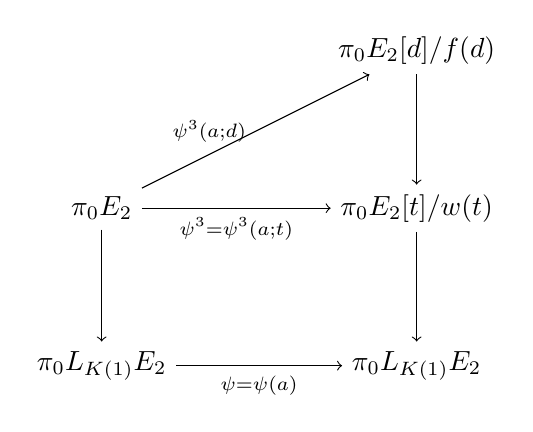
\begin{tikzpicture}
	\node (LT) at (0, 2) {$\pi_0 E_2$};
        \node (LB) at (0, 0) {$\pi_0 L_{K(1)} E_2$};
	\node (RT) at (4, 2) {$\pi_0 E_2 [t] / w(t)$};
	\node (RB) at (4, 0) {$\pi_0 L_{K(1)} E_2$};
	\node (RT0) at (4, 4) {$\pi_0 E_2 [d] / f(d)$};
	\draw [->] (LT) -- node [below] {$\scriptstyle \psi^3 = \psi^3(a;t)$} (RT); 
	\draw [->] (LB) -- node [below] {$\scriptstyle \psi = \psi(a)$} (RB); 
	\draw [->] (LT) -- node [left] {$\scriptstyle \psi^3(a;d)$} (RT0); 
	\draw [->] (LT) -- (LB); 
	\draw [->] (RT) -- (RB);
	\draw [->] (RT0) -- (RT);
\end{tikzpicture}
\end{center}

Problem explained in [po].

There is a formula for $\psi^3(a)$ in terms of $d$:

$-1/((-4 + a) (4 + a)) (-126 a + 28 a^3 - a^5 + 120 d - 9 a^2 d +
   3 a^4 d + 258 a d^2 - 67 a^3 d^2 + 3 a^5 d^2 - 152 d^3 +
   208 a^2 d^3 - 40 a^4 d^3 + a^6 d^3 + 198 a d^4 - 33 a^3 d^4 -
   3 a^5 d^4 + 8 d^5 + 63 a^2 d^5 - 15 a^4 d^5 + 70 a d^6 -
   17 a^3 d^6 + 24 d^7 - 6 a^2 d^7).$

There is a quartic polynomial $w(t)$ satisfied by $t = 1/x = e/d = g(d)/d$:
\[
 t^4 + 3 t^3 + 3 t^2 + (1 + 4/(a^2)) t + 3/(a^2).
\]
There is a quardratic polynomial about $d$ in terms of $t$, obtained from the equation of the elliptic curve:
\[
 (t + 1) d^2 - a t (t + 1) d - t.
\]
Use Mathematica to reduce the above three and get a formula for $\psi^3(a)$ in terms of $t$:
\[
 (t + 1)^3 a^3 - (4 t + 3) a,
\]
which is $a^3$ mod 3. This ``is the total power operation we'd been pursuing'', period.\\

\hrule

- (\texttt{3-K(1).nb}) \textbf{The $K(1)$-local power operation}

Solve for $t$ 3-adically from
\[
 w(t) = t^4 + 3 t^3 + 3 t^2 + (1 + 4/(a^2)) t + 3/(a^2),
\]
namely, first writing 
\[
 t = -\frac{1}{a^2 + 4}(a^2 t^4 + 3 a^2 t^3 + 3 a^2 t^2 + 3),
\]
and then substituting $t$ recursively.

Plug this value into $\psi^3(a;t)$ and we get the $K(1)$-local power operation $\psi(a)$.

Also, since $\psi^3$ is a ring homomorphism, we have a formula for $\psi^3(h;t)$:
\[
 (t + 1)^3 h^3 - (22 t^3 + 69 t^2 + 75 t + 27) h^2 + (128 t^3 + 424 t^2 + 512 t + 201) h - 16 (14 t^3 + 49 t^2 + 65 t + 27).
\]
We can do the same as above by rewriting
\[
 w(t;h) = t^4 + 3 t^3 + 3 t^2 + (1 + 4/(h-4)) t + 3/(h-4).
\]\\

\hrule

- (\texttt{level3(alpha).nb}) \textbf{The coefficient $\alpha$ - seeking for the right parameter of $\psi^3$}

Recall that 
\[
 u' = u(P) u(P-Q) u(P+Q) = \alpha u + \cdots,
\]
where 
\[
 \alpha = -\frac{1}{(-4 + a) (4 + a)}(-18 - 12 a d + 2 d^2 + a^2 d^2 
 - 15 a d^3 + 4 a^3 d^3 + 2 d^4 + a^2 d^4 + a^4 d^4 
\]
\[
 - 6 a d^5 + 3 a^3 d^5 - 2 d^6 + 3 a^2 d^6 + a d^7) 
 ~~~~~~~~~~~~~~~~~~~~~~~~~~~~~~~~~~~~~~~~~
\]
\[
 = a g(d) - d^2.  
 ~~~~~~~~~~~~~~~~~~~~~~~~~~~~~~~~~~~~~~~~~~~~~~~~~~~~~~~~~~~~~~~~~~~~~~~~~~~~
\]
This $\alpha$ is invariant under {\em any} change of coordinates (cf [Wed-4/13/11, p2]) -- FALSE. 
For future application $\alpha$ becomes quite important.  
By the way, as a uniformizer (cf p18 of AEC) at the identity (a simple zero modulo 3), 
$u$ can be taken as a complex orientation; in particular, $\pi_0 E_2 ({\mb CP}^\infty) = \pi_0 E_2 \llbracket u \rrbracket$.  
$\A$ is invariant under {\em strict} isomorphisms $w = u + a_2 u^2 + \cdots$.  

Now, by the blackbox Mathematica method, we reduce
\[
 \alpha = \alpha(a,d),
\]
\[
 (t+1)d^2-at(t+1)d-t=0,
\]
\[
 w(t)=0,
\]
and get the relation between $\alpha$ and $t$
\[
 \alpha = 3 + a^2 t + 2 a^2 t^2 + a^2 t^3.
\]
\[
 (\beta = 3 \textcolor{blue}{~+~t~} + a^2 t \textcolor{blue}{~-~t^2~} + 2 a^2 t^2 + a^2 t^3)
\]
Is $\alpha$ the right parameter of $\psi$? We next reduce
\[
 \psi(h) = \psi(h,t),
\]
\[
 \alpha = 3 + a^2 t + 2 a^2 t^2 + a^2 t^3,
\]
\[
 w(t)=0,
\]
and get 

$\psi(h, \alpha) = \frac{1}{a^2}(3120 - 432 a^2 + 2848 \alpha + 144 \alpha^2 - 480 \alpha^3 - 1536 h + 
 201 a^2 h - 1288 \alpha h - 48 \alpha^2 h + 216 \alpha^3 h + 225 h^2 - 
 27 a^2 h^2 + 168 \alpha h^2 + 3 \alpha^2 h^2 - 28 \alpha^3 h^2 - 9 h^3 +
  a^2 h^3 - 6 \alpha h^3 + \alpha^3 h^3)$

together with a surprising byproduct
\[
 t = -\frac{\alpha}{1+\alpha}.
\]
We check directly using the expressions of $t$ and $\alpha$ in terms of $a$ and $d$ that the above relation is indeed true. 
Thus, as $t = 1/x$, $\alpha$ is a certain coordinate (!)
\[
 \alpha = -\frac{1}{x}\left(1+\frac{1}{x}+(\frac{1}{x})^2+\cdots\right).
\]
Moreover, via this, $w(t) = 0$ translates to
\[
W(\alpha) := \alpha^4 - 6\alpha^2 + (a^2-8)\alpha-3 = 0.                                            
\]


\newpage
\section{Structure of $E$-\DL algebra}

\subsection{Formulas}

(\texttt{Q-alpha.nb}) 

$A = K(2)$-local commutative $E$-algebra.

Define $Q_0, Q_1, Q_2, Q_3\co\pi_0A \to \pi_0A$ by
\[
 \psi^3 (x) = Q_0(x) + Q_1(x) \alpha + Q_2(x) \alpha^2 +Q_3(x) \alpha^3,
\]
where $\alpha$ satisfies
\[
 W(\alpha) = \alpha^4 - 6\alpha^2 + (a^2-8)\alpha-3 = 0.
\]
Note: formulas change if use $t$ instead of $\alpha$ (more denominators would appear, hard to find the Adem relations, etc.).

Commutation relations ({\em twist}):

$Q_0(h x) = (h^3 - 36 h^2 + 390 h - 1212) Q_0(x) + (3 h^2 - 72 h + 360) Q_1(x) + (9 h - 108) Q_2(x) + 24 Q_3(x)$,

$Q_1(h x) = (-6 h^2 + 144 h - 712) Q_0(x) + (-18 h + 228) Q_1(x) + (-72) Q_2(x) + (h - 12) Q_3(x)$,

$Q_2(h x) = (3 h - 36) Q_0(x) + 8 Q_1(x) + 12 Q_2(x) + (-24) Q_3(x)$,

$Q_3(h x) = (h^2 - 24 h + 120) Q_0(x) + (3 h - 36) Q_1(x) + 8 Q_2(x) + 12 Q_3(x)$;

$Q_0(a x) = (a^3 - 12 a + 12 a^{-1}) Q_0(x) + (3 a - 12 a^{-1}) Q_1(x) + (12 a^{-1}) Q_2(x) + (-12 a^{-1}) Q_3(x)$,

$Q_1(a x) = (-6 a + 20 a^{-1}) Q_0(x) + (-20 a^{-1}) Q_1(x) + (- a + 20 a^{-1}) Q_2(x) + (4 a - 20 a^{-1}) Q_3(x)$,

$Q_2(a x) = (4 a^{-1}) Q_0(x) + (-4 a^{-1}) Q_1(x) + (4 a^{-1}) Q_2(x) + (- a - 4 a^{-1}) Q_3(x)$,

$Q_3(a x) = (a - 4 a^{-1}) Q_0(x) + (4 a^{-1}) Q_1(x) + (-4 a^{-1}) Q_2(x) + (4 a^{-1}) Q_3(x)$.

Adem relations ({\em product}): 

$\alpha' = - \alpha^3 + 6 \alpha - h + 12$ (cf end of section 3 on p7 of [h2p2]),

$\Psi(x) = Q_0Q_0(x) + (-h + 12) Q_0Q_1(x) + (h^2 - 24 h + 126) Q_0Q_2(x) + \textcolor{blue}{(-3)} Q_1Q_1(x) + (-h^3 + 36 h^2 - 396 h + 1296) Q_0Q_3(x) + (3h - 36) Q_1Q_2(x) + (-3 h^2 + 72 h - 378) Q_1Q_3(x) + 9 Q_2Q_2(x) + (-9 h + 108) Q_2Q_3(x) + (-27) Q_3Q_3(x)$,

$Q_1Q_0(x) = (-6) Q_0Q_1(x) + (6 h - 72) Q_0Q_2(x) + (-6 h^2 + 144 h - 747) Q_0Q_3(x) + 18 Q_1Q_2(x) + 3 Q_2Q_1(x) + (-18 h + 216) Q_1Q_3(x) + (-54) Q_2Q_3(x) + (-9) Q_3Q_2(x)$,

$Q_2Q_0(x) = (-3) Q_0Q_2(x) + (3 h - 36) Q_0Q_3(x) + 9 Q_1Q_3(x) + 3 Q_3Q_1(x)$,

$Q_3Q_0(x) = Q_0Q_1(x) + (-h + 12) Q_0Q_2(x) + (h^2 - 24 h + 126) Q_0Q_3(x) + (-3) Q_1Q_2(x) + (3 h - 36) Q_1Q_3(x) + 9 Q_2Q_3(x)$.

Cartan formulas ({\em coproduct}):

$Q_0(xy) = Q_0(x) Q_0(y) + 3 [Q_1(x) Q_3(y) + Q_2(x) Q_2(y) + Q_3(x) Q_1(y)] + 18 Q_3(x) Q_3(y)$,

$Q_1(xy) = [Q_0(x) Q_1(y) + Q_1(x) Q_0(y)] + (-h + 12) [Q_1(x) Q_3(y) + Q_2(x) Q_2(y) + Q_3(x) Q_1(y)] + 3 [Q_2(x) Q_3(y) + Q_3(x) Q_2(y)] + (-6h + 72) Q_3(x) Q_3(y)$,

$Q_2(xy) = [Q_0(x) Q_2(y) + Q_1(x) Q_1(y) + Q_2(x) Q_0(y)] + 6 [Q_1(x) Q_3(y) + Q_2(x) Q_2(y) + Q_3(x) Q_1(y)] + (-h + 12) [Q_2(x) Q_3(y) + Q_3(x) Q_2(y)] + 39 Q_3(x) Q_3(y)$,

$Q_3(xy) = [Q_0(x) Q_3(y) + Q_1(x) Q_2(y) + Q_2(x) Q_1(y) + Q_3(x) Q_0(y)] + 6 [Q_2(x) Q_3(y) + Q_3(x) Q_2(y)] + (-h + 12) Q_3(x) Q_3(y)$.

Additivity:

$Q_i(x+y) = Q_i(x) + Q_i(y)$.

Action on scalars:

$Q_0(1) = 1, Q_1(1) = Q_2(1) = Q_3(1) = 0$;

$Q_0(h) = h^3 - 36 h^2 + 390 h - 1212$,

$Q_1(h) = -6 h^2 + 144 h - 712$,

$Q_2(h) = 3 h - 36$,

$Q_3(h) = h^2 - 24 h + 120$;

$Q_0(a) = a^3 - 12 a + 12 a^{-1}$,

$Q_1(a) = -6 a + 20 a^{-1}$,

$Q_2(a) = 4 a^{-1}$,

$Q_3(a) = a - 4 a^{-1}$.

Frobenius congruence:

$Q_0(x) \equiv x^3~\text{mod}~3$,

$\theta\co\pi_0A \to \pi_0A$ such that $Q_0(x) = x^3 + 3 \theta(x)$.\\


\newpage
\subsection{Reduction mod $p$}
\label{subsec:Qmodp}

To recognize more patterns, it might be helpful to reduce the formulas modulo 3 or $(3,h)$ (interplay with operations at lower height).

Commutation relations (mod 3), cf [mc1, 4.10]:

$Q_0(h x) \equiv h^3 Q_0(x)$,

$Q_1(h x) \equiv -Q_0(x) + h Q_3(x)$,

$Q_2(h x) \equiv -Q_1(x)$,

$Q_3(h x) \equiv h^2 Q_0(x) - Q_2(x)$;

at the prime 2,

$Q_0(a x) \equiv a^2 Q_0(x)$,

$Q_1(a x) \equiv -Q_0(x) + a Q_2(x)$,

$Q_2(a x) \equiv a Q_0(x) - Q_1(x)$.

Moreover we have: 

at the prime 3, 
\begin{equation*}
\begin{split}
 Q_0 h \equiv & ~ (h^3 + h^2 + h) Q_0 + (h^2 + 1) Q_1 + (h + 1) Q_2 \md 2, \\
       \equiv & ~ (h^3 + 3 h^2 + h + 3) Q_0 + (3 h^2 + h + 1) Q_1 - (h + 1) Q_2 \md 5, \\
 Q_1 h \equiv & ~ Q_1 + (h + 1) Q_3 \md 2, \\
       \equiv & ~ (-h^2 + 3 h + 1) Q_0 + (-3 h + 1) Q_1 + 3 Q_2 + (h + 1) Q_3 \md 5, \\
 Q_2 h \equiv & ~ (h + 1) Q_0 + Q_2 \md 2, \\
       \equiv & ~ (3 h + 3) Q_0 + 3 Q_1 - Q_2 + Q_3 \md 5, \\
 Q_3 h \equiv & ~ (h^2 + 1) Q_0 + (h + 1) Q_1 + Q_3 \md 2, \\
       \equiv & ~ (h^2 - 3 h - 3) Q_0 + (3 h + 3) Q_1 + 3 Q_2 - Q_3 \md 5; 
\end{split}
\end{equation*}
at the prime 2,
\begin{equation*}
\begin{split}
 Q_0 a \equiv & ~ a^2 Q_0 + a Q_1 \md 3, \\
       \equiv & ~ a^2 Q_0 - 2 a Q_1 + Q_2 \md 5, \\
 Q_1 a \equiv & ~ a Q_2 \md 3, \\
       \equiv & -2 Q_0 + a Q_2 \md 5, \\
 Q_2 a \equiv & ~ 2 a Q_0 \md 3, \\
       \equiv & -a Q_0 - 2 Q_1 \md 5.  
\end{split}
\end{equation*}

Adem relations (mod 3, mod $(3,h)$): 

$Q_1Q_0(x) \equiv 0 \equiv 0$,

$Q_2Q_0(x) \equiv 0 \equiv 0$,

$Q_3Q_0(x) \equiv Q_0Q_1(x) - h Q_0Q_2(x) + h^2 Q_0Q_3(x) \equiv Q_0Q_1(x)$;

at the prime 2,

$Q_1Q_0(x) \equiv 0 \equiv 0$,

$Q_2Q_0(x) \equiv Q_0Q_1(x) + a Q_0Q_2(x) \equiv Q_0Q_1(x)$.

Cartan formulas (mod 3, $\equiv$ usual one mod $(3,h)$):

$Q_0(xy) \equiv Q_0(x) Q_0(y)$,

$Q_1(xy) \equiv [Q_0(x) Q_1(y) + Q_1(x) Q_0(y)] - h [Q_1(x) Q_3(y) + Q_2(x) Q_2(y) + Q_3(x) Q_1(y)]$,

$Q_2(xy) \equiv [Q_0(x) Q_2(y) + Q_1(x) Q_1(y) + Q_2(x) Q_0(y)] - h [Q_2(x) Q_3(y) + Q_3(x) Q_2(y)]$,

$Q_3(xy) \equiv [Q_0(x) Q_3(y) + Q_1(x) Q_2(y) + Q_2(x) Q_1(y) + Q_3(x) Q_0(y)] - h Q_3(x) Q_3(y)$;

(using the parameter $t$ (\texttt{Q-t.nb}): $\equiv$ messier mod 3, $\equiv$ usual one mod $(3,h)$)

at the prime 2,

$Q_0(xy) \equiv Q_0(x) Q_0(y)$,

$Q_1(xy) \equiv [Q_0(x) Q_1(y) + Q_1(x) Q_0(y)] + a [Q_1(x) Q_2(y) + Q_2(x) Q_1(y)]$,

$Q_2(xy) \equiv [Q_0(x) Q_2(y) + Q_1(x) Q_1(y) + Q_2(x) Q_0(y)] + a Q_2(x) Q_2(y)$.


\newpage
\subsection{A uniform presentation of the \DL algebra for Morava $E$-theory at height 2}
\label{uniform}

\begin{itemize}
 \item Bring in the Hecke algebra structure ($T_p \A = h$).  
 Hecke operator and involution commute [Atkin-Lehner, lemma 11].  

 \item Modify $\mf A_2$ (lift from height 1 to height 2).  
 The $K(1)$-local case.  

 \item $\todo$ Instability relations for $E$-theory power operations on the space level [lpo, Steenrod] 
\end{itemize}


\subsubsection{Formulas}

\subsubsection*{p = 2}

$A_0 = \BZ_2 \lb \textcolor{red}{a} \rb$ 

$A_1 = \BZ_2 \lb a, d \rb / (d^3 - a d - 2) 
= \BZ_2 \lb d, d' \rb / (d d' + 2) 
= \BZ_2 \lb a, a' \rb / ((a^2 - a') (a - a'^2) + 2 (5 a a' - 27))$ 

$d^3 - a d - 2 = 0$ \hfill $(-2)^2 - a d'^2 + d'^3 = 0$ 

$d^3 - a d - 2 \equiv \textcolor{brown}{d (d^2 - a)} \md 2$ 

$d' = \frac{-2}{d} = -d^2 + a$ 

$\textcolor{blue}{T_2 d} = \sum \frac{-2}{d_i} = \sum \frac{-d_1 d_2 d_3}{d_i} 
~\textcolor{red}{= a} ~\textcolor{blue}{= d^2 + d'}$ 

$a' = d'^2 + d = a^2 + 3 d - a d^2$ 

$\textcolor{blue}{T_2 a} = \sum a_i' = a^2$ 
\hfill $\textcolor{blue}{a^2 + a'} = a^2 + (a^2 + 3 d - a d^2) \equiv a^2 + \textcolor{brown}{(a^2 + 3 \cdot 0 - a \cdot a)}\footnote{$a' = T_2 d' \approx \sum d_i = 0$; 
in general, $h' = T_p \A' \approx \sum \A_i \equiv 0 \md p$ (cf $\G_1(4)$ at $p = 5$).  } = a^2 \textcolor{blue}{\mod 2}$ ?  


\subsubsection*{p = 3}

$A_0 = \BZ_9 \lb \textcolor{red}{h} \rb$ 

$A_1 = \BZ_9 \lb h, \A \rb / (\A^4 - 6 \A^2 + (h - 9) \A - 3) 
= \BZ_9 \lb \A, \A' \rb / (\A \A' + 3) 
= \BZ_9 \lb h, h' \rb / ((h^3 - h') (h - h'^3) + 3 (\text{messy}))$ 

$\A^4 - 6 \A^2 + (h - 9) \A - 3 = 0 \hfill (-3)^3 - 6 (-3) \A'^2 + (h - 9) \A'^3 + \A'^4 = 0$ 

$\A^4 - 6 \A^2 + (h - 9) \A - 3 \equiv \textcolor{brown}{\A (\A^3 + h)} \md 3$ 

$\A' = \frac{-3}{\A} = -\A^3 + 6 \A - h + 9$ 

$\textcolor{blue}{T_3 \A} = \sum \frac{-3}{\A_i} = \sum \frac{\A_1 \cdots \A_4}{\A_i} 
~\textcolor{red}{= -h + 9} = \A^3 - 6\A + \A' ~\textcolor{blue}{\equiv \A^3 + \A' \md 3}$ 

$h' = 9 - \A'^3 + 6 \A' - \A = h^3 - 27 h^2 + 201 h - 342 + (-6 h^2 + 108 h - 334) \A + (3 h - 27) \A^2 + (h^2 - 18 h + 57) \A^3$ 

$\textcolor{blue}{T_3 h} = \sum h_i' = h^3 - 27 h^2 + 183 h -153 \equiv h^3 \md 3$ 

\hfill $\textcolor{blue}{h^3 + h'} \equiv h^3 + (h^3 - \A + h^2 \A^3) \equiv h^3 + \textcolor{brown}{(h^3 - 0 + h^2 (-h))} = h^3 \textcolor{blue}{\mod 3}$ ?  


\subsubsection*{p = 5}
\label{formula5}

$A_0 = \BZ_{5^4} \lb \textcolor{red}{h} \rb$ ?  

$\G_1(3)$: \hfill [Sun-12/15/13] 

$\A^6 - 5 a \A^4 + 40 \A^3 - 5 a^2 \A^2 + h \A - 5 = 0 \hfill h = a^4 - 19 a$ 

$\A^6 - 5 a \A^4 + 40 \A^3 - 5 a^2 \A^2 + h \A - 5 \equiv \textcolor{brown}{\A (\A^5 + h)} \md 5$ 

$\A' = \frac{-5}{\A} = -\A^5 + 5 a \A^3 - 40 \A^2 + 5 a^2 \A - h$ 

$\textcolor{blue}{T_5 \A} = \sum \frac{-5}{\A_i} = \sum \frac{\A_1 \cdots \A_6}{\A_i} 
~\textcolor{red}{= -h} = \A^5 - 5 a \A^3 + 40 \A^2 - 5 a^2 \A + \A' ~\textcolor{blue}{\equiv \A^5 + \A' \md 5}$ 

$\G_1(4)$: \hfill [Mon-12/16/13], \texttt{h'.nb} 

$\A^6 - 10 \A^5 + 35 \A^4 - 60 \A^3 + 55 \A^2 - h \A ~\textcolor{green}{+}~ 5 = 0$ 

\hfill $5^5 - 10 \cdot 5^4 \A' + 35 \cdot 5^3 \A'^2 - 60 \cdot 5^2 \A'^3 + 55 \cdot 5 \A'^4 - h \A'^5 + \A'^6 = 0$ 

$\A^6 - 10 \A^5 + 35 \A^4 - 60 \A^3 + 55 \A^2 - h \A + 5 \equiv \textcolor{brown}{\A (\A^5 - h)} \md 5$ 

$\A' = \frac{\textcolor{green}{+}5}{\A} = -\A^5 + 10 \A^4 - 35 \A^3 + 60 \A^2 - 55 \A + h$ 

\hfill $y^2 + a x y + a y = x^3 + x^2$ with $h = a^4 - a^2 + 1 = 0$\footnote{Note that this is not defined over $\BF_5$ (cf [AEC,V.2.3.1b] and [KM, 2.6.3]); 
over $\BF_5$, $y^2 = x^3 + 1$ is ``standard'' supersingular [AEC, V.4.4] with $(2,2)$ a 6-torsion point fixed by $\Frob$.  } 

\hfill $(0,0)$ a 4-torsion point, fixed by $\Frob$ 

\hfill $[5](0,0) = (0,0) = \Frob^2(0,0)$ 

\hfill $\psi' \circ \psi = [5]$ 

$\textcolor{blue}{T_5 \A} = \sum \frac{5}{\A_i} = \sum \frac{\A_1 \cdots \A_6}{\A_i} 
~\textcolor{red}{= h} = \A^5 - 10 \A^4 + 35 \A^3 - 60 \A^2 + 55 \A + \A' ~\textcolor{blue}{\equiv \A^5 + \A' \md 5}$ 
\begin{equation*}
\begin{split}
 h' = & ~ \A'^5 - 10 \A'^4 + 35 \A'^3 - 60 \A'^2 + 55 \A' + \A \\
    = & ~ h^5 - 10 h^4 - 1065 h^3 + 12690 h^2 + 168930 h - 1462250 + (-55 h^4 + 850 h^3 + 39575 h^2 - 608700 h - 1113524) \A \\
      & + (60 h^4 - 775 h^3 - 45400 h^2 + 593900 h + 2008800) \A^2 + (-35 h^4 + 400 h^3 + 27125 h^2 - 320900 h - 1418300) \A^3 \\
      & + (10 h^4 - 105 h^3 - 7850 h^2 + 86975 h + 445850) \A^4 + (-h^4 + 10 h^3 + 790 h^2 - 8440 h - 46680) \A^5 
\end{split}
\end{equation*}
$\textcolor{blue}{T_5 h} = \sum h_i' = h^5 - 10 h^4 - 1340 h^3 + 18440 h^2 + 267430 h - 3178240 \equiv h^5 \md 5$ 

\hfill $\textcolor{blue}{h^5 + h'} \equiv h^5 + (h^5 + \A - h^4 \A^5) \equiv h^5 + \textcolor{brown}{(h^5 + 0 - h^4 \cdot h)} = h^5 \textcolor{blue}{\mod 5}$ ?  


\subsubsection{New model}
\label{new}

$E^0 = A_0 = \BZ_{p^2} \lb h \rb$ 

$E^0 B\Sigma_p / I = A_1 = \BZ_{p^2} \lb \A, \A' \rb / (\A \A' + p)\footnote{for a ``standard supersingular curve over $\BF_{p^2}$'' } 
= \BZ_{p^2} \lb h, \A \rb / (w(\A))$ 

$\textcolor{red}{h = T_p \A}$ ~~\qquad $A_1$ as a left $A_0$-module 
\hfill \href{http://mathoverflow.net/a/19399}{Eichler-Shimura}: $\textcolor{blue}{T_p \equiv F + V \md p}$ 

$\textcolor{brown}{h' = T_p \A'}$ \qquad $A_1$ as a right $A_0$-module [mc1, p15] 
\hfill $\displaystyle (C,G) \mapsto \sum_{\psi \co\! C \to C'} (C',\psi(G))$ 

What can we say, then?  [Wed-6/25/14] 
\hfill viewpoint for $w(\A)$: monomials correspond to isogenies 

The congruence $w(\A) \equiv \A (\A^p \pm h) \md p$, 
with $h$ an obstruction to supersingularity, 
forces $h$ to be the linear coefficient in $w(\A)$, 
and thus the identification with $T_p \A$.  

Do we have an inverse to the Hecke operator?  See \href{http://en.wikipedia.org/wiki/Iwahori\%E2\%80\%93Hecke_algebra\#Properties}{here}.  

If we take into account the action of Hecke operators 
($T_p \A$ gives the generator $h$---Hecke operators on modular forms of higher level [Wed-4/16/14]) 
perhaps we can then give a uniform presentation of the \DL algebra at height 2 [Mon-6/30/14].  

Still, $T_p$ is supposed to preserve weight.  
Learn more about Hecke operators, weight, level, ... 


\subsubsection{Old model}
\label{subsubsec:old}

$E^0 = A_0 = \BZ_{p^2} \lb x \rb$ 

$E^0 B\Sigma_p / I = A_1 
= \textcolor{gray}{\BZ_{p^2} \llbracket x, \A \rrbracket \big/ \big( \A (\A^p - x) - p \big)} 
= \BZ_{p^2} \llbracket \A, \A' \rrbracket / (\A \A' + p) 
= \BZ_{p^2} \llbracket x, x' \rrbracket \big/ \big( (x^p - x') (x - x'^p) + p (\cdots) \big)$ with 
\[
 \textcolor{gray}{x = \A^p + \A'} 
\]
(and $x' = \A'^p + \A$)---compatibility between the $E_\infty$-ring spectrum and its power operations 

The left $A_0$-module structure on $A_1$: free of rank $p+1$ on the basis $1, \A, \ldots, \A^p$ with 
\[
 \A'^n = x^n - \sum_{i=1}^n (-p)^{n-i} x^{i-1} \A^{p-n+i} \qquad \qquad 1 \leq n \leq p+1 
\]
and $\A^{p+1} = p + x \A$ 

The dual basis for $\G_1 = A_1^*$: $Q_0, Q_1, \ldots, Q_p$ with 
\[
 \psi^p = Q_0 + Q_1 \A + \cdots + Q_p \A^p 
\]

The total power operation 
\[
 \psi^p (x) = \psi^p (\A^p + \A') = \A'^p + \A = x^p - \sum_{i=1}^p (-p)^{p-i} x^{i-1} \A^i + \A \equiv x^p \md (p,\A) 
\]

Commutation relations:

$Q_k c = c^{(p)} Q_k \qquad \qquad c \in \BZ_{p^2}$

$\displaystyle Q_0 x = \sum_{i=0}^p (-p)^i x^{p-i} Q_i + p Q_p$

$Q_1 x = \big( 1- (-p)^{p-1} \big) Q_0 + x Q_p$

$\displaystyle Q_k x = \sum_{i=0}^{k-1} -(-p)^{p-k+i} x^{k-i-1} Q_i + Q_{k-1} \qquad \qquad 1 < k \leq p$

Adem relations:

$\displaystyle Q_k Q_0 = (-p)^{p-k} \sum_{i=0}^{k-1} \sum_{j=0}^{k-i-1} (-p)^j x^{k-j-i-1} Q_j Q_{p-i} - \sum_{i=1}^{p-k} (-p)^i Q_{k+i} Q_i \qquad 1 \leq k \leq p$ 

with $\displaystyle \Psi = \sum_{i=0}^p \sum_{j=0}^i (-p)^j x^{i-j} Q_j Q_i$ \\

\hrule

$x$ is related to the Hasse invariant $h$ at $p$.  

The norm $\A = u(Q) u(2Q) \cdots u((p-1)Q)$ depends on the coordinate $u$.  

(Current choice doesn't work at $p = 3$.  
Suppose $h = \sum_{n=0}^\infty c_n x^n$ in $A_0$; look at its left action on $1 \in A_1$: \\
$h = -x + 6 \A + 9 = -x - 2 \A^2 \A' + \A^2 \A'^2 = -x - 2 \A^2 (x - \A^3) + \A^2 (x^2 - 2 \A^3 x + \A^6) = \cdots$) 

We know $h \equiv -\A' \md (p,\A) = (\A)$ by [KM, 12.4.1] (cf [p3, remark 3.4]).  Not always, but they are related... 

More about the Hasse invariant (without modulo $\A$)?  

More about the defining equation for the order $p$ subgroup (or $M(\G_1(N),\G_0(p))$)?  \\
$b \K^3 - \textcolor{Maroon}{a} \K - \textcolor{Maroon}{2}$ from $b u^3 - a u - 2$ 

$b^4 \K^4 - 6 b^2 \K^2 + (\textcolor{Maroon}{a^2 - 8 b}) \K - \textcolor{Maroon}{3}$ 
from $b^4 u^8 + 3 a b^3 u^7 + 3 a^2 b^2 u^6 + (a^3 b + 7 a b^2) u^5 + (6 a^2 b - 6 b^2) u^4 + 9 a b u^3 + (-a^2 + 8 b) u^2 - 3 a u - 3$ 

$b^8 \K^6 - 5 a b^5 \K^4 + 40 b^4 \K^3 - 5 a^2 b^2 \K^2 + (\textcolor{Maroon}{a^4 - 19 a b}) \K - \textcolor{Maroon}{5}$ 
from $\ldots$ ($\G_1(3)$ [Sun-12/15/13]) \\
$b^{12} \K^6 - 10 b^{10} \K^5 + 35 b^8 \K^4 - 60 b^6 \K^3 + 55 b^4 \K^2 - (\textcolor{Maroon}{a^4 - 16 a^2 b + 26 b^2}) \K + \textcolor{Maroon}{5}$ 
from $\ldots$ ($\G_1(4)$ [Mon-12/16/13]) 

The definition of $\K$ as a norm relates it to only the highest symmetric polynomial.  

Modulo $p$ the equation becomes $\A (\A^p - h) = 0$: formal part + etale part.  

\begin{enumerate}[\bf {Possibility} 1]
 \item There might be a recursive formula for these polynomials just as for division polynomials.  

 \item Other coefficients (modular forms) from Pearson's document?  \\
 \textcolor{white}{.} \hfill action of Hecke operators \\
 Their existence related to the fact that our formal group law is not nice enough (eg $p$-typical)?  \\
 \textcolor{white}{.} \hfill standard generic formal groups 
\end{enumerate}

Look into Lubin's canonical subgroups paper.  
{\em Standard generic formal groups} (pp105-6), 
Theorem E (p119, expression for $\mf A_2$: 
write down an isomorphism to $A_1$ as $E_0$-modules, 
or rather, find a relationship between them---describe a map $A_1 \to \mf A_2$).  

p = 2: 

We have 
\begin{equation*}
\begin{split}
 A_1 \cong & ~ \BZ_2 \lb a, d \rb / (d (d^2 - a) - 2) \\
     \cong & ~ \BZ_2 \lb a, a' \rb / ((a^2 - a') (a - a'^2) + 2 (5 a a' - 27)) \\
     \cong & ~ \BZ_2 \lb d, d' \rb / (d d' + 2) 
\end{split}
\end{equation*}
as modules over $\BZ_2 \lb a \rb$ (be careful about the two inclusions $A_0 \to A_1$).  
We want to study the structure of 
\[
 \mf A_2 \cong \BZ_2 \lb t, t', s \rb / (t t' - 2, t^3 s - 4) 
\]
as a module over $\BZ_2 \lb t \rb \cong \BZ_2 \lb a \rb$.  
Rationally, we have 
\[
 t' = \frac{2}{t} 
\]
\[
 s = \frac{4}{t^3} = \frac{t'^3}{2} \quad \left( s = \frac{p^p}{t^{p+1}} = \frac{t'^{p+1}}{p} \right) 
\]


\subsubsection{[can]}
\label{subsubsec:can}

At all primes and all heights, a certain universal ring $\mf A_h$, $h > 1$, appears in theorem E on p119, explicitly [Mon-4/28/14] 
\[
 {\mf A_2} \cong \BZ_p \llbracket t, \frac{p}{t}, \frac{p^p}{t^{p+1}} \rrbracket 
\]
\[
 {\mf A_h} \cong \BZ_p \llbracket t_1, t_2, \ldots, t_{h-1}, \frac{p}{t_1}, \frac{p^p t_2}{t_1^{p+1}} \rrbracket \qquad h \geq 3 
\]
\[
 \text{``${\mf A_1}$''} \cong \BZ_p \qquad (p = t_0) 
\]
(note that only $t_1$ can be ``inverted''---read [E2K], how $E$-theory to $K$-theory goes).  
The moduli problem discussed in this paper isn't quite the same (stronger) as what we were looking at for a total power operation: 
it is about a ``canonical'' lift of Frobenius (p107), 
in contrast to the $p+1$ subgroups any of which we may choose as the kernel for the ``universal'' deformation/lift of Frobenius.  
\textcolor{red}{a single $\A$ ($\A_0$?) vs $\A_0, \A_1, \ldots, \A_p$} 

However, at height 2 the formal Laurent series $\pi(t)$ in that theorem might correspond to the $K(1)$-local power operation described in the last section of [p3]: 
there, we have 
\begin{equation}
\label{h}
 \begin{split}
  \p_F(h) = & ~ h^3 - 27 h^2 + 183 h - 180 + 186 h^{-1} + 1674 h^{-2} + 13878 h^{-3} \\
            & + 103518 h^{-4} + 537597 h^{-5} - 2419551 h^{-6} - 151959321 h^{-7} \\
            & - 3641020389 h^{-8} - 71654526828 h^{-9} - 1300181743908 h^{-10} \\
            & - 22630101262848 h^{-11} - 384618396177288 h^{-12} \\
            & - 6442799277467304 h^{-13} - 106938529542815688 h^{-14} \\
            & - 1764499704722922168 h^{-15} - 29002794605762488344 h^{-16} \\
            & - 475539362099470239246 h^{-17} - 7785153453939122671326 h^{-18} \\
            & - 127339438683160404062298 h^{-19} - 2081954101607845046438274 h^{-20} \cdots 
 \end{split}
\end{equation}
and $\pi(t)$ is an element in 
\[
 \BZ_p \lb t, \frac{p}{t}, \frac{p^p}{t^{p+1}} \rb 
\]
with $h$ corresponding to $t$ (modulo $p$ and up to a unit).  
In other words, to get the $K(1)$-local power operation $\p_F$, we were using the {\em canonical} subgroup of order 3 
(simply because there's a unique order-3 subgroup at height 1), 
and this subgroup corresponds to the unique value of $\A$ that is substituted into $\p(h;\A)$ to get $\p_F(h)$.  
Comparing the two moduli problems, there should be a classifying map 
\[
 \BZ_9 \llbracket h, \A \rrbracket / (\A^4 - 6 \A^2 + (h - 9) \A - 3) \to \BZ_9 \llbracket t, \frac{3}{t}, \frac{27}{t^4} \rrbracket 
\]
which sends $h$ to $t$, and $\A$ to 
\begin{equation*}
 \begin{split}
  \text{``}\A = & ~ (3 + 6 \A^2 - \A^4) \sum_{n=1}^\infty 9^{n-1} h^{-n} = \cdots \text{''} \\
              = & ~ 3 t^{-1} + 27 t^{-2} + 297 t^{-3} + 3645 t^{-4} + 47790 t^{-5} \cdots 
 \end{split}
\end{equation*}
We have diagrams 
\begin{equation}
\label{A_2}
 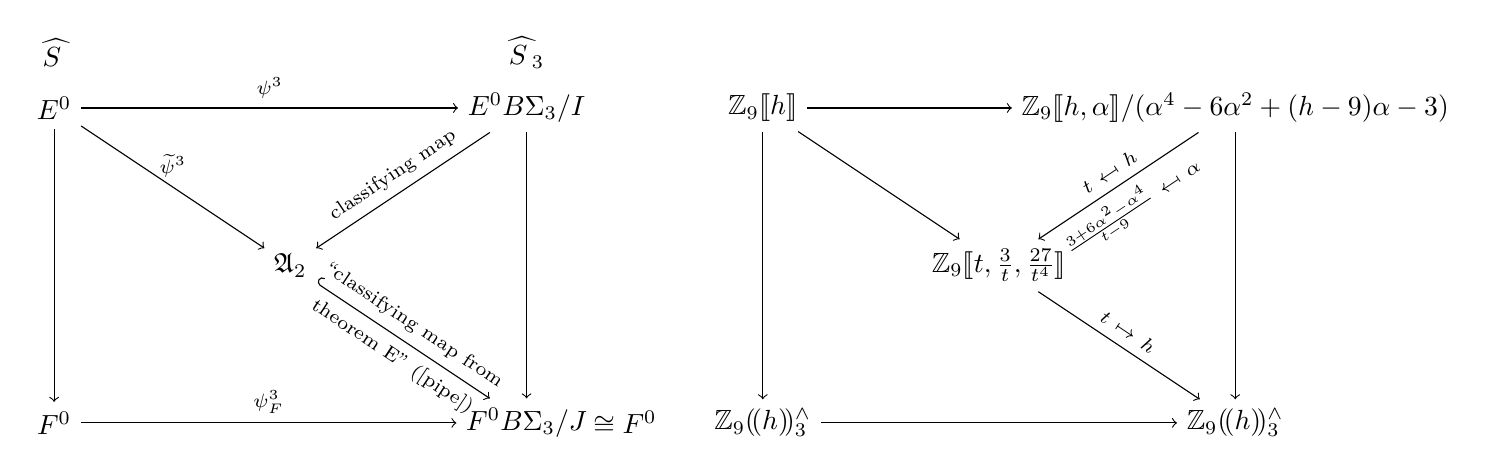
\begin{tikzpicture}[baseline=(current bounding box.center)]
         \node (LT) at (0, 4) {$E^0$}; 
         \node at (0, 4.7) {$\HS$}; 
         \node (RT) at (6, 4) {$E^0 B\Sigma_3 / I$}; 
         \node at (6, 4.7) {$\HS_3$}; 
         \node (LB) at (0, 0) {$F^0$}; 
         \node (MB) at (6, 0) {$F^0 B\Sigma_3 / J$}; 
         \node (C) at (3, 2) {${\mf A_2}$}; 
         \node (RB) at (7.25, 0) {$\cong F^0$}; 
         \draw [->] (LT) -- node [above] {$\scriptstyle \p$} (RT); 
         \draw [->] (LT) -- (LB); 
         \draw [->] (RT) -- (MB); 
         \draw [->] (LB) -- node [above] {$\scriptstyle \psi_F^3$} (MB); 
         \draw [->] (LT) -- node [above] {$\scriptstyle \Tp^3$} (C); 
         \draw [->] (RT) -- node [above,sloped] {$\scriptstyle \text{classifying map}$} (C); 
         \draw [right hook->] (C) -- node [above,sloped] {$\scriptstyle \text{``classifying map from}$} 
                                     node [below,sloped] {$\scriptstyle \text{theorem E'' ([pipe])}$} (MB); 
         \node (LT1) at (9, 4) {$\BZ_9 \lb h \rb$}; 
         \node (RT1) at (15, 4) {$\BZ_9 \lb h, \A \rb / (\A^4 - 6 \A^2 + (h - 9) \A - 3)$}; 
         \node (LB1) at (9, 0) {$\BZ_9 (\!( h )\!)^\wedge_3$}; 
         \node (MB1) at (15, 0) {$\BZ_9 (\!( h )\!)^\wedge_3$}; 
         \node (C1) at (12, 2) {$\BZ_9 \lb t, \frac{3}{t}, \frac{27}{t^4} \rb$}; 
         \draw [->] (LT1) -- (RT1); 
         \draw [->] (LT1) -- (LB1); 
         \draw [->] (RT1) -- (MB1); 
         \draw [->] (LB1) -- (MB1); 
         \draw [->] (LT1) -- (C1); 
         \draw [->] (RT1) -- node [above,sloped] {$\scriptstyle t ~\mapsfrom~ h$} 
                             node [below,sloped] {$\scriptstyle \frac{3 + 6 \A^2 - \A^4}{t - 9} ~\mapsfrom~ \A$} (C1); 
         \draw [->] (C1) -- node [above,sloped] {$\scriptstyle t ~\mapsto~ h$} (MB1); 
 \end{tikzpicture}
\end{equation}
where the map 
\[
 E^0 \to F^0 \xrightarrow{\psi^3_F} F^0 \qquad \text{lifts to} \qquad \Tp^3 \co E^0 \to \mf A_2 
\]
Computational evidence for $\psi^p_F(h) \in \mf A_2$ (in the absence of \href{http://tinyurl.com/jwtr2ba}{Atkin}): 
\begin{itemize}
 \item [p = 3] (\texttt{h1p3\_alpha\_h\_-20.nb}) We checked $\p_F(h)$ \eqref{h} down to $h^{-20}$ (first 24 terms): 
 the coefficients all contain sufficently many 3-factors, 
 precisely as many for the negative powers 1, 3, 5, 9, 13, 15, 17 of $h$; 
 the same conclusion (including those 7 specific negative powers) holds for $\A(h)$ down to $h^{-22}$.  

 \item [p = 2] (\texttt{2-K(1)\_a\_-52.nb}) We checked $\psi^2_F(a)$ down to $a^{-52}$ (first 19 terms): 
 \begin{equation*}
 \begin{split}
  \psi^2_F(a) = & ~ a^2 - 10 a^{-1} - 56 a^{-4} - 736 a^{-7} - 12288 a^{-10} - 230912 a^{-13} \\
                & - 4659200 a^{-16} - 98598912 a^{-19} - 2159149056 a^{-22} \\
                & - 46508277760 a^{-25} - 979219513344 a^{-28} - 20256129024000 a^{-31} \\
                & - 413760095256576 a^{-34} - 8374930945081344 a^{-37} \\
                & - 168325239044833280 a^{-40} - 3363201507053797376 a^{-43} \\
                & - 66848486735870951424 a^{-46} - 1322432066183409696768 a^{-49} \\
                & - 26047337841215500451840 a^{-52} \cdots 
 \end{split}
 \end{equation*}
 the coefficients all contain sufficently many 2-factors, 
 precisely as many for the negative powers 1, 4, 7, 13, 16, 28, 31, 34, 43, 49 of $a$; 
 the same conclusion (including those 10 specific negative powers) holds for $d(a)$ down to $a^{-52}$.  

 \item [p = 5] (\texttt{5-K(1)\_h\_-7.nb}) We checked $\psi^2_F(h)$ down to $h^{-7}$ (first 13 terms): 
 \begin{equation*}
 \begin{split}
  \psi^5_F(h) = & ~ h^5 - 10 h^4 - 1340 h^3 + 18440 h^2 + 267430 h - 3178250 \\
                & - 920120 h^{-1} + 183770000 h^{-2} - 11467367375 h^{-3} \\
                & + 449827523750 h^{-4} - 16654435175000 h^{-5} \\
                & + 595612985750000 h^{-6} - 21005686830531250 h^{-7} \cdots 
 \end{split}
 \end{equation*}
 the coefficients all contain sufficently many 5-factors, 
 precisely as many for the negative powers 3, 4, 5, 7 of $h$; 
 the same conclusion (including those 4 specific negative powers together with $-9$ and $-10$) holds for $\A(h)$ down to $h^{-11}$.  \\
\end{itemize}

\hrule

In general, by Strickland's generalization of Lubin-Tate, we have an {\em injection} 
\begin{equation*}
\begin{split}
 \BZ_{p^2} \lb h, \A \rb / (w(\A)) \to & ~ \BZ_{p^2} \lb t, \frac{p}{t}, \frac{p^p}{t^{p+1}} \rb \\
 h \mapsto & ~ t \\
 \A \mapsto & ~ \A_0(h=t) \qquad \qquad \qquad \qquad \text{numerical evidence} 
\end{split}
\end{equation*}
On the other hand, by theorem E, with the setup 

\begin{tabular}{cccccc}
 $\mf A_2$ & over & $\BZ_p$ & $\subset$ & $\BQ_p$ & \\
 && $\cap$ && $\cap$ & \\
 $\mf A_2'$ & over & $A_0 = \BZ_{p^2} = \BZ_p[i]$ & $\subset$ & $K_0 = \BQ_{p^2} = \BQ_p(i)$ & \\
 && $\cap$ && $\cap$ & not a {\em finite} extension as required \\
 && $A = \BZ_{p^2} \lb h, \A \rb / (w(\A))$ & $\subset$ & $K = \BQ_{p^2} \lp h, \A \rp / (w(\A))$ & 
\end{tabular}

get (not quite, see [p-prop, 3.4] and \eqref{A_2}) 
\begin{equation*}
\begin{split}
 {\mf A_2'} = \BZ_{p^2} \lb t, \frac{p}{t}, \frac{p^p}{t^{p+1}} \rb \to & ~ \BZ_{p^2} \lb h, \A \rb / (w(\A)) \\
 t \mapsto & ~ h \textcolor{gray}{\thinspace + \cdots} 
\end{split}
\end{equation*}
or 
\begin{equation*}
\begin{split}
 \BZ_{p^2} \lb t, t', s \rb / (t t' - p, t^{p+1} s - p^p, \textcolor{red}{t s - t'^p}) \to & ~ \BZ_{p^2} \lb h, \A, \A' \rb / (w(\A), \A \A' + p) \\
 t \mapsto & ~ \A' \textcolor{gray}{\thinspace + \cdots} \\
 t' \mapsto & -\A \textcolor{gray}{\thinspace + \cdots} \\
 s \mapsto & ~ \frac{1}{1 + w_p \A^{-1} + \cdots + w_2 \A^{-(p-1)} - h \A^{-p}} \\
 & \qquad \qquad \qquad \qquad \text{needs $\A$ inverted, or weaker, adjoining $\frac{p^\text{small}}{\A^\text{large}}$} \\
 \equiv & ~ 1 - \frac{h}{\A'} \md p \qquad \qquad \qquad \quad \text{cf ~ $w(\A) \equiv \A \textcolor{red}{(\A^p - h)} \md p$} 
\end{split}
\end{equation*}
Moreover, we have a {\em surjection} (cf [h2, 9.14]) 

\begin{tabular}{ccc}
 ${\mf A_2'} / p = $ & $\BF_{p^2} \lb t, t', s \rb /$ & $(t t', t^{p+1} s, t s - t'^p)$ \\
 & $\uparrow$ & $\cup$ \\
 & $\BF_{p^2} \lb t, t', s \rb /$ & $((t - t'^p) (t^p - t') s)$ 
\end{tabular}

Good things about $\mf A_2$: 
\begin{itemize}
 \item Has a uniform presentation for $p$ and $h$.  

 \item Is a classifying object.  

 \item Seems to be somewhere between height 1 and height 2 (cf \eqref{A_2} and [Fri-7/4/14]).  
\end{itemize}

Want: Lift (?) $\mf A_2$ to $A_1$.  

Need: Understand the parameters of $\mf A_2$, especially $s$ (cf [Fri-6/27/14, Wed-7/2/14]).  \\

\hrule

Questions: 
\begin{itemize}
 \item Would the ring $\mf A_h$ be something interesting in the context of $E$-\DL algebra?  

 \item Specifically, at height 2, could $\mf A_2$ be promoted as the target ring of a kind of ``canonical'' total power operation, 
 in the form 
 \begin{equation}
 \label{tt's}
  \BZ_{p^2} \llbracket t, t', s \rrbracket / (t t' - p, t^{p+1} s - \textcolor{red}{p^p}), 
 \end{equation}
 which descends to the {\em same} power operation $\p_F$ at height 1 as the total power operation $\p$?  
 How far is the classifying map $E^0 B\Sigma_3 / I \to {\mf A_2}$ in \eqref{A_2} from being an isomorphism [Wed-2/11/15]?  
 It is injective.  

 Compare \eqref{tt's} with our known presentations for $E^0 B\Sigma_p / I$ [Sat-3/22/14, Tue-3/25/14]: 
 \begin{itemize}
  \item[-] $\textcolor{red}{p^p}$ shows up as the constant term in the degree-$(p+1)$ polynomial 
  satisfied by $\A'$---the parameter for the noncanonical subgroups / etale part, 
  possibly another ``deformation parameter'' along with the Hasse invariant 
  ($w(\A) \equiv \A (\A^p \pm h) \md p$, and $h \equiv \mp \A' \md \A$).  
  Thus the classifying map $E^0 B\Sigma_3 / I \to {\mf A_2}$ in \eqref{A_2} may be equivalently defined by 
  \[
   \A' \mapsto t 
  \]
  \[
   \A \mapsto -\frac{3}{t} 
  \]
  \[
   h = 9 - \A^3 + 6 \A - \A' \mapsto -t + 9 - \frac{18}{t} + \frac{27}{t^3} 
  \]
  For it to be surjective, we have the generator $\frac{27}{t^4}$ in 
  \[
   3^3 - 6 \cdot 3 \A'^2 - (h - 9) \A'^3 - \A'^4 = 0 
  \]
  that is, 
  \[
   \frac{27}{t^4} - 2 \A^2 - \frac{h - 9}{t} - 1 = 0 
  \]
  and in general there is always a term $\frac{h}{t}$ 
  so that the surjectivity needs $\A'$ to be genuinely inverted 
  (not just having $\frac{3}{\A'}$), ie ``canonical'' as opposed to ``universal.''  
  Is there a way to modify this generator and get an isomorphism?  

  \item[-] In \eqref{tt's} we have relations 
  \[
   t'^p = t s \qquad\qquad t'^{p+1} = p s 
  \]
 \end{itemize}

 \item Is $\mf A_2$ realizable?  
\end{itemize}


\newpage
\subsubsection{Cusps}
\label{subsubsec:cusps}

Origin: section \ref{subsubsec:h-opr}, [ho, example 6.7] 

Idea: \texttt{w\_i.nb}, [Thu-3/5/15 meeting] 

Historical documents: [Wed-10/10/12], Kubert's table, [KM, $\pi$150] 

Proof: [Sat-4/4/15] 
we need $\A$ because it is the norm parameter for the moduli problem, invariant under $\G_0(p)$ 

Lift from cusps: fix $p$, vary $N$ 
\begin{enumerate}[(i)]
 \item {[Sun-4/5/15]} $N = p - 1$ 
 \begin{itemize}
  \item $\G_1(6)$: [Wed-3/18/15] 

  \item $\G_1(6)$ at 7: [Thu-3/19/15, Sat-4/4/15] 
 \end{itemize}

 \item {[Mon-4/13/15, Tue-4/14/15, Thu-4/16/15]} 
 Thoughts after canonical modular polynomials: complication at larger genera?  
 \begin{itemize}
  \item {[Mon-4/20/15 meeting]} Canonical modular polynomials 
  (\rd{difference from $j = 744$ equals $\#\Aut(E_\text{s.s.}/\cF_p)$}; 
  constant terms equal $p^s$ where $s = 12 / \gcd(p - 1, 12) \stackrel{?}{=} \prod (\#\Aut(E_\text{s.s.}/\cF_p)/2)$) 
  \begin{equation*}
   \begin{split}
     X_0(2) \qquad & ~ x^3+48 x^2+(\rd{768-j}) x+2^{12} \\
            \equiv & ~ x (x^2 - j) \md 2 \\
     X_0(3) \qquad & ~ x^4+36 x^3+270 x^2+(\rd{756-j}) x+3^6 \\
            \equiv & ~ x (x^3 - j) \md 3 \\
     X_0(5) \qquad & ~ x^6+30 x^5+315 x^4+1300 x^3+1575 x^2+(\rd{750-j}) x+5^3 \\
            \equiv & ~ x (x^5 - j) \md 5 \\
     X_0(7) \qquad & ~ x^8+28 x^7+322 x^6+1904 x^5+5915 x^4+8624 x^3+4018 x^2+(\rd{748-j}) x+7^2 \\
            \equiv & ~ x (x^7 - (j + 1)) \md 7 \\
    X_0(13) \qquad & ~ x^{14}+26 x^{13}+325 x^{12}+2548 x^{11}+13832 x^{10}+54340 x^9+157118 x^8 \\
                   & +333580 x^7+509366 x^6+534820 x^5+354536 x^4+124852 x^3+15145 x^2 \\
                   & +(\rd{746-j}) x+13^1 \\
            \equiv & ~ x (x^{13} - (j - 5)) \md 13 \\
    X_0(11) \qquad & ~ x^{12}-5940 x^{11}+14701434 x^{10}+(-139755 j-19264518900) x^9 \\
                   & +(723797800 j +13849401061815) x^8+(67496 j^2-1327909897380 j \\
                   & -4875351166521000) x^7+(2291468355 j^2+1036871615940600 j \\
                   & +400050977713074380) x^6+(-5346 j^3+4231762569540 j^2 \\
                   & -310557763459301490 j+122471154456433615800) x^5+(161201040 j^3 \\
                   & +755793774757450 j^2+17309546645642506200 j \\
   \end{split}
  \end{equation*}
  \begin{equation*}
   \begin{split}
                   & +6513391734069824031615) x^4+(132 j^4-49836805205 j^3 \\
                   & +6941543075967060 j^2-64815179429761398660 j \\
                   & +104264884483130180036700) x^3+(468754 j^4+51801406800 j^3 \\
                   & +214437541826475 j^2+77380735840203400 j+804140494949359194) x^2 \\
                   & +(-j^5+3732 j^4-4586706 j^3+2059075976 j^2-253478654715 j \\
                   & +2067305393340) x+11^6 \\
            \equiv & ~ x (x^{11} - j^2 (j - 1)^3) \md 11 \\
    X_0(17) \qquad & ~ x^{18}+510 x^{17}+125001 x^{16}+19248080 x^{15}+2058738420 x^{14}+(10846 j \\
                   & +160172066760) x^{13}+(6027384 j+9242645403716) x^{12}+(1273189500 j \\
                   & +396142696578480) x^{11}+(149639194520 j+12417332467452654) x^{10} \\
                   & +(-2601 j^2+10935992495298 j+274068816038694900) x^9+(13895953 j^2 \\
                   & +512956753613040 j+3930522394593478542) x^8+(-6334200306 j^2 \\
                   & +15050663748715720 j+29822585665567020720) x^7+(582813995247 j^2 \\
                   & +249498731117744880 j+25265814014664728452) x^6+(102 j^3 \\
                   & -12771700921226 j^2+1855481229180865218 j \\
                   & -782798617139667376440) x^5+(304164 j^3+57276026369631 j^2 \\
                   & +3208047335393719960 j+1674871156833326914740) x^4+(14192620 j^3 \\
                   & -30176599785714 j^2+527256473998693500 j \\
                   & -1020930937750503845680) x^3+(13396068 j^3+281395910081 j^2 \\
                   & +249471554573688 j+5170904888984217) x^2+(-j^4+2982 j^3-2547081 j^2 \\
                   & +567877726 j-8730057090) x+17^3 \\
            \equiv & ~ x (x^{17} - j (j - 8)^3) \md 17 \\
    X_0(19) \qquad & ~ x^{20}-152 x^{19}+11020 x^{18}-509732 x^{17}+16884502 x^{16}-423717176 x^{15} \\
                   & +8284685786 x^{14}+(-950 j-127757600560) x^{13}+(316312 j \\
                   & +1555736163737) x^{12}+(-30558479 j-14818816436876) x^{11} \\
                   & +(1393783456 j+107820178372660) x^{10}+(-35139121246 j \\
                   & -570206255492636) x^9+(516859448264 j+1951802961922337) x^8+(76 j^2 \\
                   & -4417019896714 j-2792663674453360) x^7+(52003 j^2 \\
                   & +20685669251624 j-6236737094541574) x^6+(3153696 j^2 \\
                   & -46304956732366 j+21913915458273064) x^5+(32293274 j^2 \\
                   & +37088471763616 j+37717059200889382) x^4+(52948896 j^2 \\
                   & -5786452184639 j+14998237694760268) x^3+(6707323 j^2 \\
                   & +24879503032 j+1299029281420) x^2+(-j^3+2236 j^2-1075910 j \\
                   & +37507528) x+19^2 \\
            \equiv & ~ x (x^{19} - (j + 1) (j - 7)^2) \md 19 
   \end{split}
  \end{equation*}

  \item $\big( [\G_0(p)], [\G_1(\ell)] \big)$ 
  \begin{equation*}
   \begin{split}
    & ~ 2 \cdot \frac{1}{24} (p + 1) (\ell^2 - 1) = 2 g - 2 + 2 (\ell - 1) \\
    \implies & ~ g = \frac{(p + 1) (\ell^2 - 1)}{24} - \ell + 2 
   \end{split}
  \end{equation*}

  \item $\big( [\G_0(p)], [\G_1(N)] \big)$ 
  \[
   \frac{p + 1}{12} N^2 \prod_{\ell | N} \left( 1 - \frac{1}{\ell^2} \right) = 2 g - 2 + 2 c(\G_1(N)) 
  \]
  where $\phi(N) \leq c(\G_1(N)) \leq N^2 \prod_{\ell | N} \left( 1 - \frac{1}{\ell^2} \right)$ 

  \item Examples of $g(p,N)$ 
  \begin{center}
   \begin{tabular}{ll}
    $g(2,3) = 0$ & \qquad good \\
    $g(3,4) = 0$ & \qquad good \\
    $g(5,3) = 1$ & \qquad bad ~~~ \rd{Three supersingular points in this case!} $-a^4 + 19 a \equiv -a (a + 1) (a^2 - a + 1)$ \\
    $g(5,4) = 1$ & \qquad good! \\
    $g(7,4) = 2$ & \qquad bad? \\
    $g(7,6) = 5$ & \qquad bad? wish to compute \\
    $g(7,3) = \dfrac{5}{3}$ & \qquad not representable? \\\\
   \end{tabular}

   \rd{``good'' because $(p - 1) (N - 1) | 12$} 
  \end{center}
 \end{itemize}
\end{enumerate}

Read [Ahlgren] and [Choi] and see how to generalize from genus-zero $\G_0(p)$, 
especially the function $\phi_p$ (appears as a parameter for the canonical modular polynomials) and nice sequences of modular functions...  


\subsubsection{Canonical modular polynomials}
\label{subsubsec:cmp}

Motivating question: What is special about genus zero?  

\begin{ex}[\texttt{eta5.nb}]
 $p = 5$ 

 $s \ce \dfrac{12}{\gcd(p - 1, 12)} = 3$ \qquad $x x' = p^s = 5^3$ 

 $u \ce \dfrac{p - 1}{\gcd(p - 1, 12)} = 1$ 

 \begin{equation*}
  \begin{split}
   x' = \phi_p(z) \ce & \left( \frac{\eta(z)}{\eta(p z)} \right)^{2 s} \\
                    = & \left( \frac{q^{1/24} \prod_{n = 1}^\infty (1 - q^n)}{q^{5/24} \prod_{n = 1}^\infty (1 - q^{5 n})} \right)^6 \\
                    = & ~ q^{-1} \left( \frac{\href{http://oeis.org/A010815}{1 - q - q^2 + q^5 + q^7 - q^{12} - q^{15} + \cdots}}{1 - q^5 - q^{10} + q^{25} + q^{35} - q^{60} - q^{75} + \cdots} \right)^6 
                        \hskip 1cm \bl{c_i} = \left\{
                        \begin{array}{ll}
                         \!\! (-1)^k & ~~ \text{if $i = k (3 k \pm 1) / 2$} \\
                         \!\! 0 & ~~ \text{otherwise} 
                        \end{array}
                        \right. \\
                    = & ~ \frac{1}{q} \, \rd{- \, 6} + 9 q + 10 q^2 - 30 q^3 + 6 q^4 -25 q^5 + 96 q^6 + 60 q^7 - 250 q^8 + 45 q^9 - 150 q^{10} + \cdots \\
                    = & ~ q^{-u} + \cdots \\
                      & \hskip -1.25cm \text{a univalent modular function on $\G_0(5)$, with a simple pole at infinity} \\
                      & \hskip -1.25cm \text{and a simple zero at 0 (the two cusps of $\G_0(p)$): [Ahlgren, p788], [web, section 1.4, esp.~theorem 1.64],} \\
                      & \hskip 6.17cm \text{[Apostol, sections 4.7-10, esp.~theorems 4.7 and 4.9]} \\
                      & \hskip 6.17cm \text{[MF, section 3.8]} 
  \end{split}
 \end{equation*}

 There exists a unique degree-$u$ polynomial $f(j)$ such that $f(j) - x'$ is a cusp form of weight 0: 
 \begin{equation*}
  \begin{split}
      j = & ~ \href{http://oeis.org/A000521}{\dfrac{1}{q} + 744 + 196884 q + 21493760 q^2 + 864299970 q^3 + 20245856256 q^4 + 333202640600 q^5 + \cdots} \\
   f(j) = & ~ j - 750 
  \end{split}
 \end{equation*}
 Moreover, note that 
 \begin{itemize}
  \item $j_0 = 750 \equiv 0$ is the unique supersingular $j$-invariant at 5 [AEC, V.4.4] 

  \item $f(j) - x' \equiv 0 \md 5$ 
 \end{itemize}
 Questions 
 \begin{itemize}
  \item Is $f(j)$ a polynomial of supersingular $j$-invariants?  Cf [Kaneko-Zagier] and [Milas-Mortenson-Ono].  

  \item Is $x'$ a Hasse invariant?  Cf [p3, remark 3.4].  
 \end{itemize}

 Following [Choi, (2.4)] (generalizing [Ahlgren, p788] generalizing [BKO, pp553-4]), we compute that\footnote{By analogy to [BKO, p553], 
 $j_5^{(5)}(z) = j_1^{(5)}(z) | T_0(5)$; in other words, $h' = T_5 x'$, which echoes $h = T_p \A$ in section \ref{new}.  } 
 \begin{equation}
  \label{jup}
  \begin{split}
   j_{u p}^{(p)}(z) = & ~ j_5^{(5)}(x',j) \\
                    = & ~ x'^5 + 30 x'^4 + 315 x'^3 + 1300 x'^2 + 1575 x' \\
                    = & ~ \frac{1}{q^5} \, \rd{- \, 6} + \rd{5} q (\cdots) \hskip 4cm \text{Why\rd{??}} 
  \end{split}
 \end{equation}
 and get 
 \begin{equation*}
  \begin{split}
   \cmp(x',j') = & ~ x' j_{u p}^{(p)} - x' \big(f(j') - x\big) \\
     \cmp(x,j) = & ~ x^6 + 30 x^5 + 315 x^4 + 1300 x^3 + 1575 x^2 + (750 - j) x + 5^3 
  \end{split}
 \end{equation*}
 In fact, more directly, adapting [Choi, (2.4)], we have 
 \[
  j_{u (p + 1)}^{(p)}(x',j\rd{'}) \text{~``$=$''~} \cmp(x',j') 
 \]
 where $j'(z) = j(p z)$.  Note that since 
 \begin{equation*}
  \begin{split}
   x' = & ~ \frac{1}{q^u} + \cdots \\
   j' = & ~ \frac{1}{q^p} + \cdots 
  \end{split}
 \end{equation*}
 and $p \!\!\not|\, u$, this algorithm {\em always} works.  

 Upshot (cf [ho, (3.10)]) 
 \begin{equation*}
  \begin{split}
                          \psi^5 \co E^0 \to & ~ E^0(B\Sigma_5) / I \\
   \BW\big(\cF_5\big)\lb h = j - 750 \rb \to & ~ \BW\big(\cF_5\big)\lb x,j \rb / \big(\cmp(x,j)\big) \\
                                   h \mapsto & ~    j' - 750 = x + \rd{1} x'^5 + \rd{30} x'^4 + \rd{315} x'^3 + \rd{1300} x'^2 + \rd{1575} x' \\
                                             & \hskip 1.35cm = x + (h - x^5 - 30 x^4 - 315 x^3 - 1300 x^2 - 1575 x)^5 + \cdots \\
                                             & \hskip 1.35cm = h^5 + 30 h^4 - 787185 h^3 - 78654950 h^2 + 113706048450 h + 9128404218750 \\
                                             & \hskip 1.75cm   + (-\rd{1575} h^4 - 209750 h^3 + 919941375 h^2 + 146313952500 h - 53794421543124) x \\
                                             & \hskip 1.75cm   + (-\rd{1300} h^4 - 78375 h^3 + 765753000 h^2 + 83642547500 h - 47590693860000) x^2 \\
                                             & \hskip 1.75cm   + (-\rd{315} h^4 - 13200 h^3 + 185819525 h^2 + 17992315500 h - 11702653105500) x^3 \\
                                             & \hskip 1.75cm   + (-\rd{30} h^4 - 1025 h^3 + 17705550 h^2 + 1622265375 h - 1120917084750) x^4 \\
                                             & \hskip 1.75cm   + (-\rd{1} h^4 - 30 h^3 + 590310 h^2 + 52436200 h - 37473142200) x^5 
  \end{split}
 \end{equation*}
 Questions 
 \begin{itemize}
  \item Can we imitate the $q$-expansion for $\phi_p(z)$ and write down one for $\A$ (or $\A'$), 
  based on the Lubin construction [ho, construction 3.1(ii)] and the formulas for $p$-torsions on the Tate curve in [padicprop, 1.11]?  
  And then carry out the above process for $(\A,h)$ in place of $(x,j)$?  

  Actually, are the $q$-expansions for $\A$ equal to $p$ around 
  the unramified cusp $\infty$, and $1$ around the ramified cusp $0$?  

  Remember that the definition of $\A$ depends on a rigidification $N > 3$.  
  Introducing $N$ may increase the number of supersingular points, 
  and $(p - 1) (N - 1)$ may or may not divide 12 (certainly not when $p = 13$).  

  \item Or, less directly, does the pattern for $\cmp(x,j)$ at genus-zero primes force the pattern for $w(\A,h)$ 
  predicted from restriction over the cusps as in section \ref{subsubsec:cusps}?  
  \[
   w(\A,h) = (\A - p) (\A - 1)^p - \big((-1)^p + p (-p) (-1)^{p - 1} + h\big) \A 
  \]
  At these primes (each with a single supersingular $j$-invariant), $j$ and $h$ are the same.  
  But again, $\A$ may not work nicely at 13.  

  We don't yet know a nice formula for the higher coefficients in $\cmp(x,j)$ [\texttt{cmp.nb}, Mon-6/8/15]: 
  \[\hskip -3.3cm
   \begin{array}{llll}
    w_p & = 2 s p & = \frac{24 p}{p - 1} & = 2 (s + 12) \\
    w_{p - 1} & = s p (2 s p - 4 s + 3) & = \frac{36 p (9 p - 17)}{(p - 1)^2} & = -(s + 12) (2 s - 27) \\
    w_{p - 2} & = \frac{2}{3} s p (2 s p - 6 s + 1) (s p - 3 s + 4) & = \frac{64 p (2 p - 5) (25 p - 73)}{(p - 1)^3} & = \frac{4}{3} (s + 12) (s - 8) (4 s - 25) \\
    w_{p - 3} & = \frac{1}{6} s p (2 s p - 8 s + 1) (2 s p - 8 s + 3) (s p - 4 s + 7) & = \frac{18 p (3 p - 11) (19 p - 55) (25 p - 97)}{(p - 1)^4} & = -\frac{1}{2} (s + 12) (2 s - 9) (3 s - 19) (6 s - 25) \\
    w_{p - 4} & = \frac{1}{15} s p (s p - 5 s + 3) (2 s p - 10 s + 3) & = \frac{576 p (5 p - 21) (9 p - 41) (34 p^2 - 275 p + 529)}{5 (p - 1)^5} & = \frac{4}{15} (s + 12) (4 s - 15) (8 s - 27) \\
              & ~~~~~~~~ (2 s^2 p^2 - 20 s^2 p + 21 s p + 50 s^2 - 105 s + 4) & & ~~~~~~~~ (8 s^2 - 69 s + 136) 
   \end{array}
  \]
 \end{itemize}

 Second attempt: write down $\psi^5(h)$ by comparing $q$-expansions 
 \begin{equation*}
  \begin{split}
   h' = & ~ j' - 750 = \frac{1}{q^5} - 6 + 196884 q^5 + \cdots \\
    h = & ~ j - 750 = \frac{1}{q} - 6 + 196884 q + \cdots \\
    x = & ~ \frac{5^3}{x'} = 125 q + 750 q^2 + 3375 q^3 + \cdots \\
   \implies \qquad & \\
   h' = & ~ h^5 + 30 h^4 - \rd{1575} h^4 x - 787185 h^3 + (-\rd{1300} h^4 x^2 + ? h^3 x + ? h^2) + \cdots 
  \end{split}
 \end{equation*}
\end{ex}

\begin{ex}[\texttt{eta11.nb}]
 $p = 11$ 

 $s = 6$ \qquad $x x' = 11^6$ 

 $u = 5$ 

 \begin{equation*}
  \begin{split}
   x' = \phi_{11}(z) = & \left( \frac{\eta(z)}{\eta(11 z)} \right)^{12} \\
                     = & ~ \frac{1}{q^5} - \frac{12}{q^4} + \frac{54}{q^3} - \frac{88}{q^2} - \frac{99}{q} + 540 - 418 q - 648 q^2 + 594 q^3 + 836 q^4 + 1056 q^5 - 4092 q^6 - 353 q^7 + \cdots \\
                       & \hskip -1.35cm \text{a modular function on $\G_0(11)$ with Nebentypus: [Apostol, pp86-7]} 
  \end{split}
 \end{equation*}

 There exists a unique $f(j)$ such that $f(j) - x'$ is a cusp form (zero modulo 11): 
 \begin{equation*}
  \begin{split}
   f(j) = & ~ j^5 - 3732 j^4 + 4586706 j^3 - 2059075976 j^2 + 253478654715 j - 2067305393340 \\
   \equiv & ~ j^2 (j - 1)^3 \md 11 \qquad\qquad\qquad\qquad\qquad\qquad\qquad\qquad\qquad\qquad\qquad\qquad \text{cf [AEC, V.4.3]} 
  \end{split}
 \end{equation*}

 Adapting [Choi, (2.4)], we compute $\cmp(x',j') \leadsto \cmp(x,j) \leadsto \cmp(x',j)$ and get 
 \begin{equation*}
  \begin{split}
   \cmp(x,j) = & ~ x^{12}-5940 x^{11}+14701434 x^{10}+(-139755 j-19264518900) x^9 \\
               & +(723797800 j +13849401061815) x^8+(67496 j^2-1327909897380 j \\
               & -4875351166521000) x^7+(2291468355 j^2+1036871615940600 j \\
               & +400050977713074380) x^6+(-5346 j^3+4231762569540 j^2 \\
               & -310557763459301490 j+122471154456433615800) x^5+(161201040 j^3 \\
               & +755793774757450 j^2+17309546645642506200 j \\
               & +6513391734069824031615) x^4+(132 j^4-49836805205 j^3 \\
               & +6941543075967060 j^2-64815179429761398660 j \\
               & +104264884483130180036700) x^3+(468754 j^4+51801406800 j^3 \\
               & +214437541826475 j^2+77380735840203400 j+804140494949359194) x^2 \\
               & +(-j^5+3732 j^4-4586706 j^3+2059075976 j^2-253478654715 j \\
               & +2067305393340) x+11^6 \\
        \equiv & ~ x \big(x^{11} - f(j)\big) \md 11 
  \end{split}
 \end{equation*}
 Directly computing $j_{55}^{(11)}(x',j)$, though doable, doesn't look good, and doesn't look right.  

 Upshot 
 \begin{equation*}
  \begin{split}
                    \psi^{11} \co E^0 \to & ~ E^0(B\Sigma_{11}) / I \\
   \BW\big(\cF_{11}\big)\lb h = j \rb \to & ~ \BW\big(\cF_{11}\big)\lb x,j \rb / \big(\cmp(x,j)\big) 
  \end{split}
 \end{equation*}
 It seems that $\BW\big(\cF_p\big)\lb x,j \rb / \big(\cmp(x,j)\big)$ is not the correct target for $E$-total power operation, 
 which arises from completion at a {\em single} supersingular point; 
 $x'$ needs to split off a factor with $q$-expansion $\dfrac{1}{q} + \cdots$, to be paired with $j$ as in the genus-zero case...  

 Thus, for all primes $p$, 
 \begin{equation*}
  \begin{split}
        \psi^p \co \big(L_{K(2)}\TMF\big)^0 \to & ~ \big(L_{K(2)}\TMF\big)^0(B\Sigma_p) / I \\
   \BW\big(\cF_p\big)\lb x' \equiv f(j) \rb \to & ~ \BW\big(\cF_p\big)\lb x', ~ j' \rb / \big(\cmp(x',j')\big) \\
                                     x' \mapsto & ~ x = -j_{u p}^{(p)}(x',j\rd{'}) + f(j') \\
                                                & \hskip .25cm = -(x')^p + \cdots \hskip 1cm \text{Frobenius class is ``$-Q_0$''} 
  \end{split}
 \end{equation*}
 Locally at each supersingular point, the above total power operation splits off a factor 
 \begin{equation*}
  \begin{split}
                          \psi^p \co E^0 \to & ~ E^0(B\Sigma_p) / I \\
   \BW\big(\cF_p\big)\lb h = j - j_0 \rb \to & ~ \BW\big(\cF_p\big)\lb h, ~ j' \rb / \big(w(h,j')\big) \qquad \text{$w(h,j')$ monic of degree $p + 1$ in $h$} \\
                                   h \mapsto & ~ h' = j' - j_0 \\
                                             & ~ \text{via {\em this} map, $E^0(B\Sigma_p) / I$ is free of rank $p + 1$ over $E^0$} 
  \end{split}
 \end{equation*}
 Compare (at genus-zero primes) 
 \begin{equation*}
  \begin{split}
   w(j - j_0, j') \equiv (j - j_0) & (j^p - j') \md p \\
   & \big(j^p - f(j')\big) ~ \text{in general} 
  \end{split}
 \end{equation*}
 to the Kronecker equation (the ``symmetrization'' of the former) 
 \[
  (j - (j')^p) (j^p - j') \equiv 0 \md p 
 \]
 Perhaps, for our purpose, the genus-zero case {\em is} the general case.  
\end{ex}

\begin{conj}[Oneida]
 The higher coefficients in $w$ remain constant (as over the cusps) 
 in a formal neighborhood of a {\em single} supersingular point, 
 so that for all $p$, we have 
 \begin{equation*}
  \begin{split}
                \psi^p \co E^0 \to & ~ E^0(B\Sigma_p) / I \\
   \BW\big(\cF_p\big)\lb h \rb \to & ~ \BW\big(\cF_p\big)\lb h, \A \rb / \big(w(h,\A)\big) 
  \end{split}
 \end{equation*}
 where 
 \begin{equation*}
  \begin{split}
   w(h,\A) = & ~ (\A - p) (\A - 1)^p - \big((-1)^p + p (-p) (-1)^{p - 1} + h\big) \A \\
      \equiv & ~ \A (\A^p - h) \md p 
  \end{split}
 \end{equation*}
 From this we can compute $\psi^p(h)$ via involution as usual algorithmically, if not explicitly, 
 which leads to a uniform presentation of the \DL algebra for Morava $E$-theory at height 2 (cf [ho, remark 6.6]).  
\end{conj}

\begin{proof}
 By Strickland, Serre-Tate, and [KM, 5.4 and 7.7], we have 
 \begin{equation*}
  \begin{split}
   & E^0(B\Sigma_p)/I \cong \BW\big(\cF_p\big)\lb h,\A \rb / \big(w(\A,h)\big) 
     ~~ \text{free of rank $p + 1$ over $E^0$} \\
   \implies & \exists ~ \text{unique monic} ~ 
              w(\A,h) = \A^{p + 1} + w_p \A^p + \cdots + w_2 \A^2 + w_1 \A + w_0 
              \qquad w_i \in E^0 \cong \BW\big(\cF_p\big)\lb h \rb \\
   & \hskip 3.63cm = \A^{p + 1} + w_p \A^p + \cdots + w_2 \A^2 - h \A + \bl{p} 
              \equiv \A (\A^p - h) \md p \\
   & \hskip 10.15cm \stackrel{\text{unrf}}{\infty} \hskip .25cm \stackrel{\text{ramified}}{0} \hskip 1.2cm \text{[padicprop, 1.13]} \\
   & \hskip 9.75cm \bl{\text{[Ando95, theorem 4] $(-1)^{p + 1} p = p$ if $p > 2$}} \\
   & \hskip 13.1cm \A_0 \A_1 \cdots \A_p = p = \A \A' 
  \end{split}
 \end{equation*}

 Imitating the derivation of a canonical modular polynomial, we have 
 \begin{equation*}
  \begin{split}
   \text{{\em single} ssing point} \implies & h = j - j_0 \\
   \implies & \A' = \frac{1}{q} + a_0 + O(q) \hskip 2cm a_0 \equiv 744 - j_0 \md p \\
   & \hskip 5.14cm \text{[KM, 12.4.1], [p3, remark 3.4] should work integrally} \\
   \implies & \exists ~ \text{constants $w_i'$ with $p|w_i'$ such that} \\
   & \quad~ (\A')^p + w_p' (\A')^{p - 1} + \cdots + w_2' \A' \\
   & = \frac{1}{q^p} + ~ \text{const} ~ + O(q) \hskip 1.54cm \text{in fact $a_0 + p O(q)$, cf \eqref{jup}} \\
   & = j' - j_0 + O(q) \hskip 2.6cm j'(z) = j(p z) \\
   & = h' + O(q) \\
   \implies & (\A')^{p + 1} + w_p' (\A')^p + \cdots + w_2' (\A')^2 
              = h' \A' + O(1) \text{---must be constant} \\
   \implies & \A^{p + 1} + w_p' \A^p + \cdots + w_2' \A^2 - h \A + p = 0 \\
   & \hskip 1.15cm \stackrel{\|}{w_p} \hskip 1.8cm \stackrel{\|}{w_2} 
  \end{split}
 \end{equation*}
 Looking at the restriction around the cusps\footnote{$h = (-1)^{p + 1} (p^2 + 1) \equiv 1 \md p$} (\ref{subsubsec:cusps}), 
 we get the values of these constants $w_i$.  
\end{proof}

How does the moduli space look?  
How close are a formal neighborhood of a supersingular point 
and a punctured disc around a cusp?  
\begin{center}
 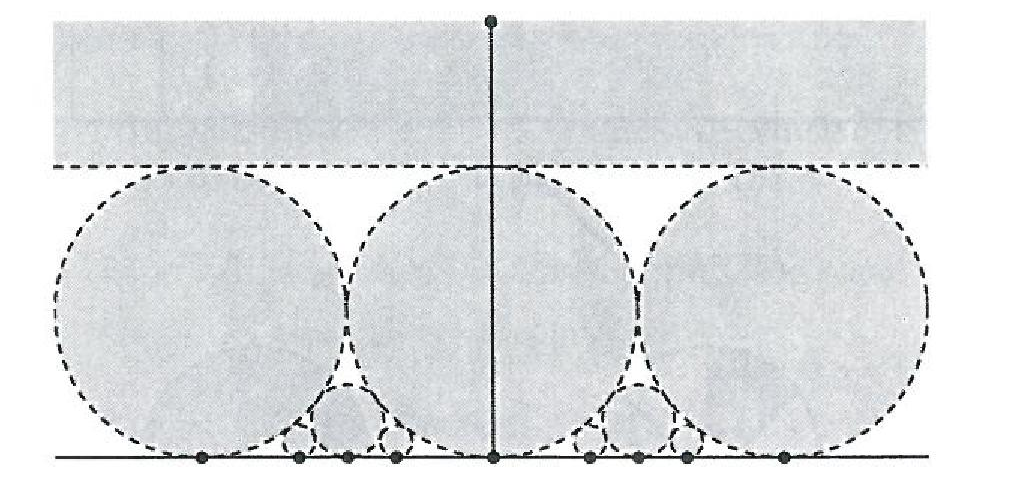
\includegraphics[scale=.37]{cusps} \\
 {\small Neighborhoods of $\infty$ and of some rational points [MF, figure 2.5]} 
\end{center}
\begin{center}
 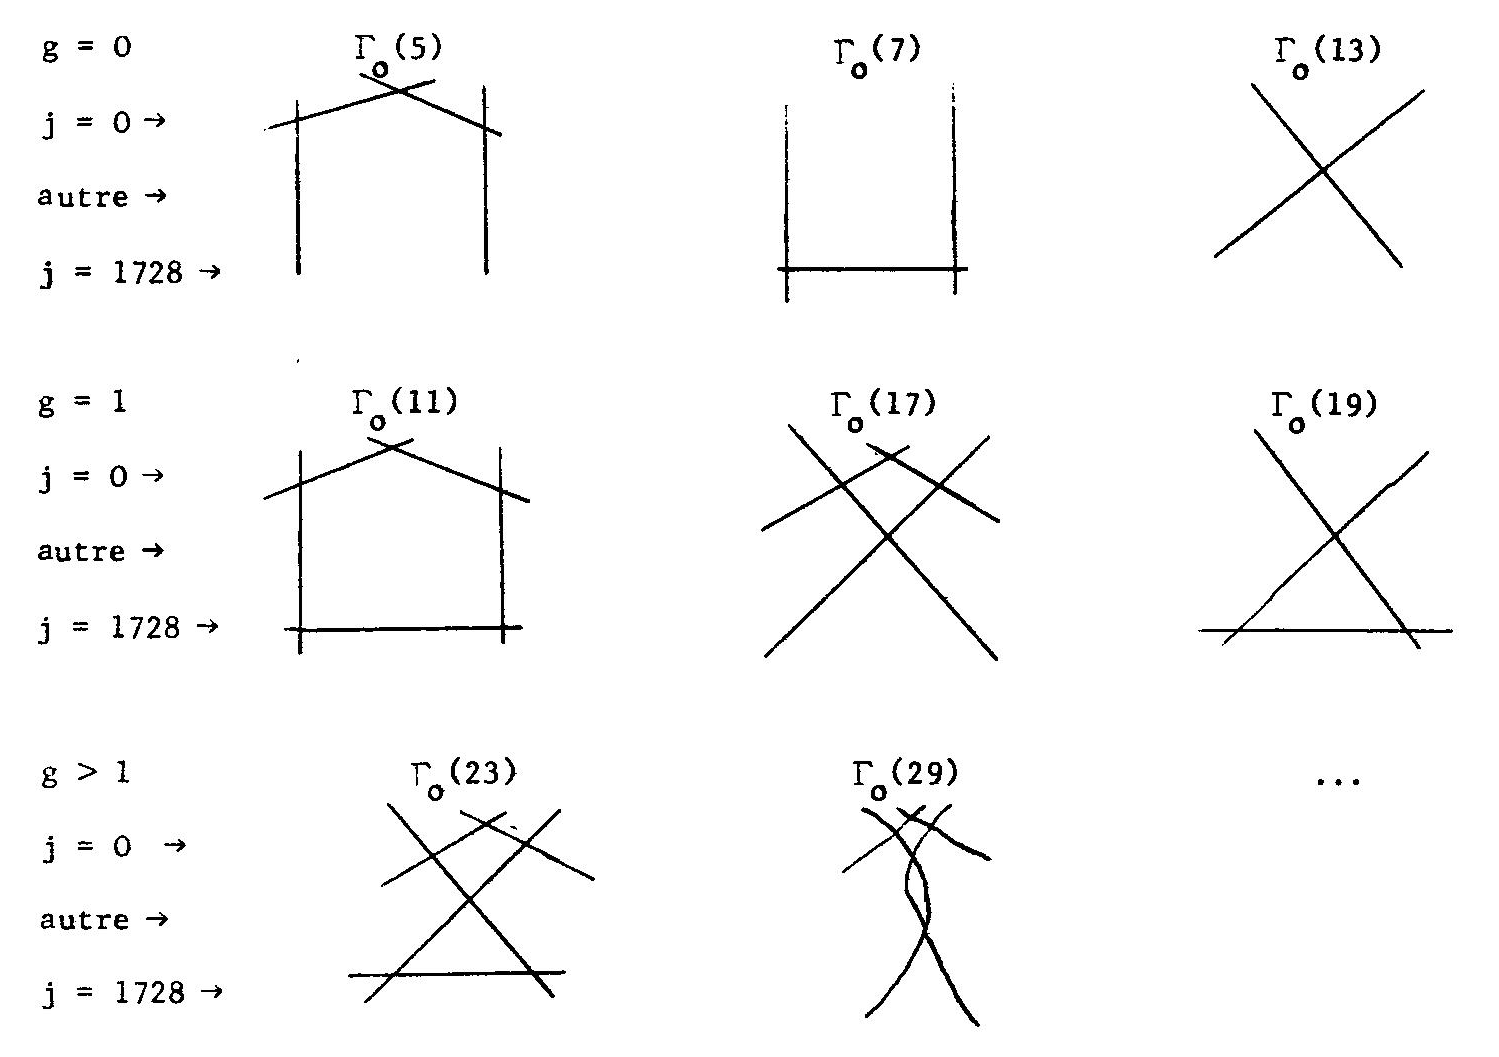
\includegraphics[scale=.24]{ssing} \\
 {\small [DR, VI.6]} 
\end{center}

\subsubsection*{Computing $\psi^p(h)$}

\begin{enumerate}[(i)]
 \item Can a computer do this with polynomials of indefinite degree?  
 \[
  \begin{split}
   (\A - p) (\A - 1)^p = & ~ (\A - p) \sum_{i = 0}^p \c{p}{i} \A^i (-1)^{p - i} \\
                       = & ~ \sum_{i = 0}^p \c{p}{i} \A^{i + 1} (-1)^{p - i} - p \sum_{i = 0}^p \c{p}{i} \A^i (-1)^{p - i} \\
                       = & ~ \sum_{j = 1}^{p + 1} \c{p}{j - 1} \A^j (-1)^{p - j + 1} - p \sum_{j = 0}^p \c{p}{j} \A^j (-1)^{p - j} \\
                       = & ~ \sum_{j = 2}^{p + 1} \left[ \c{p}{j - 1} (-1)^{p - j + 1} - p \c{p}{j} (-1)^{p - j} \right] \A^j + \cdots \\
                       = & ~ \sum_{j = 2}^{p + 1} (-1)^{p - j + 1} \left[ \c{p}{j - 1} + p \c{p}{j} \right] \A^j + \cdots \hskip 2cm \c{p}{p + 1} = 0 \\
      \implies w(\A,h) = & ~ (-p) (-1)^p - h \A + \sum_{j = 2}^{p + 1} (-1)^{p - j + 1} \left[ \c{p}{j - 1} + p \c{p}{j} \right] \A^j \\
                       = & ~ p - h \A + \sum_{j = 2}^{p + 1} (-1)^j \left[ \c{p}{j - 1} + p \c{p}{j} \right] \A^j \hskip 2.3cm \text{$p > 2$ from now on} \\
                       = & ~ p - h \A + \sum_{j = 2}^{p + 1} \left[ \c{p}{j - 1} + p \c{p}{j} \right] (-\A)^j \\
            \implies 0 = & ~ p - h \A + \sum_{j = 2}^{p + 1} \left[ \c{p}{j - 1} + p \c{p}{j} \right] \A^j \hskip 3.15cm \A \mapsto -\A, ~ h \mapsto -h \\
                       = & ~ \A^{p + 1} + 2 p \A^p + \cdots - h \A + p \\
          \implies \A' = & ~ \frac{p}{\A} \\
                       = & ~ h - \sum_{j = 2}^{p + 1} \left[ \c{p}{j - 1} + p \c{p}{j} \right] \A^{j - 1} \\
                       = & ~ h - \sum_{i = 1}^p \left[ \c{p}{i} + p \c{p}{i + 1} \right] \A^i \\
           \implies h' = & ~ \A + \sum_{k = 1}^p \left[ \c{p}{k} + p \c{p}{k + 1} \right] \left( h - \sum_{i = 1}^p \left[ \c{p}{i} + p \c{p}{i + 1} \right] \A^i \right)^k \\
                       = & ~ \A + \sum_{k = 1}^p \left[ \c{p}{k} + p \c{p}{k + 1} \right] \sum_{m_k = 0}^k \c{k}{m_k} h^{k - m_k} \left( - \sum_{i = 1}^p \left[ \c{p}{i} + p \c{p}{i + 1} \right] \A^i \right)^{m_k} \\
                       = & ~ -\A^{p^2} - 2 p^2 \A^{p^2 - 1} + \cdots + \sum_{k = 1}^p \left[ \c{p}{k} + p \c{p}{k + 1} \right] h^k 
  \end{split}
 \]

 \item Change of variables 

 Let $p > 2$ so that 
 \[
  w(\A,h) = (\A - p) (\A - 1)^p + (1 + p^2 - h) \A 
 \]
 Write 
 \[
  \left\{
  \begin{split}
   \B = & ~ \A - 1 \hskip 3.45cm \text{a unit} \\
    x = & ~ p^2 - h 
  \end{split}
  \right.
 \]
 so that 
 \[
  \begin{split}
   (1 + \B - p) \B^p + (1 + x) (1 + \B) = & ~ 0 \\
   \big( 1 - (1 + \B') \big) \B^p + 1 + x = & ~ 0 \\
   1 + x = & ~ \B^p \B' \hskip 2cm \text{multiplicativity of units} \\
   x' = & ~ (\B')^p \B - 1 \\
      = & ~ \left( \frac{x + 1}{\B^p} \right)^p \B - 1 \\
      = & ~ \frac{(x + 1)^p}{\B^{p^2 - 1}} - 1 
  \end{split}
 \]
 Reducing $\B^{p^2 - 1}$ and then inverting it is complicated [Sun-6/28/15].  Also, 
 \[
  \begin{split}
   & \hskip -1cm \left\{
     \begin{array}{l}
      \B^{p + 1} + (1 - p) \B^p + (1 + x) \B + (1 + x) = \B^p (\B + 1 - p) + (1 + x) (\B + 1) \\
      \B^p = (1 + x) (\B + 1) \cdot (1 + x)^{-1} (\B^{p - 1} - \B^{p - 2} + \B^{p - 3} - \cdots + 1) - 1 
     \end{array}
     \right. \\
   \implies ~\, 1 = & -\B^p (\B + 1 - p) \cdot (1 + x)^{-1} (\B^{p - 1} - \B^{p - 2} + \B^{p - 3} - \cdots + 1) - \B^p \\
     \implies \B' = & ~ \frac{1 + x}{\B^p} \\
                  = & -(\B + 1 - p) (\B^{p - 1} - \B^{p - 2} + \B^{p - 3} - \cdots + 1) - (1 + x) \\
                  = & -\B^p + \rd{p} \B^{p - 1} - \rd{p} \B^{p - 2} + \rd{p} \B^{p - 3} - \cdots + \rd{p} - 1 - (1 + x) 
  \end{split}
 \]
 Reducing the $p$'th power of this is hard.  

%  More promisingly, 
%  \[
%   \begin{split}
%    x' = & ~ (\B')^p \B - 1 \\
%       = & ~ (\B')^p \left( \frac{p}{\B' + 1} - 1 \right) - 1 
%   \end{split}
%  \]
%  where $\B'$ satisfies 
%  \[
%   \begin{split}
%    & ~ w(\A,h) = (\A - p) (\A - 1)^p + (1 + p^2 - h) \A \\
%    \cdot \frac{p^p}{\A^{p + 1}} \implies & ~ (\A' - 1) (\A' - p)^p + (1 + p^2 - h) (\A')^p = 0 \\
%    \implies & ~ \B' (\B' - p + 1)^p + (1 + x) (\B' + 1)^p = 0 \\
%    \implies & ~ 0 = (\B')^{p + 1} + \sum_{j = 1}^p \left[ \c{p}{j - 1} (1 - p)^{p - j + 1} + (1 + x) \c{p}{j} \right] (\B')^j + (1 + x) \\
%             & ~~\, \eqqcolon (\B')^{p + 1} + \sum_{j = 1}^p a_j (\B')^j + (1 + x) 
%   \end{split}
%  \]
%  We have 
%  \[
%   (\B')^{p + 1} + \cdots + (1 + x) = (\B' + 1) Q(\B') + R 
%  \]
%  where 
%  \[
%   \begin{split}
%    Q(\B') = & ~ (\B')^p + (a_p - 1) (\B')^{p - 1} + (a_{p - 1} - a_p + 1) (\B')^{p - 2} + (a_{p - 2} - a_{p - 1} + a_p - 1) (\B')^{p - 3} + \cdots \\
%             & + (a_1 - a_2 + a_3 - \cdots + a_p - 1) (\B')^{p - p} \\
%         R = & ~ 1 + x - (a_1 - a_2 + a_3 - \cdots + a_p - 1) \\
%           = & ~ 1 + x - (-p^p + 1 + 1 + x - 1) \\
%           = & ~ \rd{p^p} 
%   \end{split}
%  \]
%  Thus 
%  \[
%   x' = -(\B')^p \left( \frac{Q(\B')}{p^{p - 1}} + 1 \right) - 1 
%  \]
%  It remains to reduce $(\B')^p Q(\B')$.  \\

 Other changes of variables into good form (like \ref{subsubsec:old}) with reasonable involution?  
\end{enumerate}

\subsubsection{More about $\phi_p$}
\label{subsubsec:morephip}

In view of the construction of $\phi_p$ from $\D$, 
it is not surprising that $\phi_p$ has vanishing $p$-Serre derivative [Ahlgren, section 4]: 
\begin{equation*}
 \begin{split}
       & ~ \text{``$G_p \ce \frac{\theta \phi_p}{\phi_p} + \frac{p E_2 | V(p) - E_2}{p - 1} = 0$''} \\
  \iff & ~ \rd{\vartheta}_p \rd{\phi_p} \ce \rd{D\phi_p \, +} \left( \rd{\frac{k / 12 - h}{p - 1} \, \cdot \,} p \rd{\CE_2} | V(p) 
           \rd{\, + \, \frac{h - p k / 12}{p - 1} \cdot \CE_2} \right) \rd{\phi_p} = 0 
 \end{split}
\end{equation*}
where weight $k = 0$, $h = -u = -1$ [Ahlgren, lemma 2.2].  
This generalizes to all primes in [Choi, theorem 3.4].  
In fact, there is a version of $p$-Serre derivative for each $(l,p)$-type sequence $\{g_m^{(p)}\}$.\footnote{Sequences of modular functions: 
\begin{center}
 \begin{tabular}{llllll}
  $[$BKO$]$       & $\SL_2(\BZ)$       & $\{j_m(z)\}$       & $(-1,1)$-type & $j_1(z) = j(z) - 744$                        & $H_\tau(z)$ ~~~ Hauptfunktionen?  \\
  $[$Ahlgren$]$   & $\G_0(p), ~ g = 0$ & $\{j_m^{(p)}(z)\}$ & $(-1,p)$-type & $j_1^{(p)}(z) = \phi_p(z) \equiv f(j) \md p$ & $H_\tau^{(p)}(z)$ \\
  $[$Choi, 2.4$]$ & $\G_0(p), ~ g > 0$ & $\{j_m^{(p)}(z)\}$ & $(-u,p)$-type & $j_1^{(p)}(z) = j(z)$                        & \\
                  &                    &                    &               & $j_u^{(p)}(z) = \phi_p(z) \equiv f(j) \md p$ & \\
  $[$Choi, 3.1$]$ & $\G_0(N)$          & $\{g_m^{(N)}(z)\}$ & $(l,p)$-type  &                                              & $[g_m^{(N)}]_\tau(z), ~ [g_m^{(N)}]_t(z), ~ [g_m^{(N)}]_\infty(z)$ 
 \end{tabular}
\end{center}
}

It is illegitimate to deduce from this and [ho, theorem 4.13] that 
\begin{equation*}
 \begin{split}
  \ell_{2,p}(x') = & ~ \frac{1}{p} \log \frac{(x')^p \cdot x'}{x_0 \cdots x_p} \\
                 = & ~ \frac{1}{p} \log \frac{(x')^{p + 1}}{p^s} 
 \end{split}
\end{equation*}
must then be zero, because $\phi_p$ is not on $\G_1(N)$ and is not a unit either!  

However, this does seem to make sense $K(1)$-locally.  
Recall from [can] (section \ref{subsubsec:can}) that the universal ring parametrizing {\em canonical} (degree-$p$) subgroups is 
\[
 {\mf A_2} \cong \BZ_p \left\lb t, \frac{p}{t}, \frac{p^p}{t^{p+1}} \right\rb 
           \sim \BZ_p \left\lb \A, \A', \frac{(\A')^{p + 1}}{p} \right\rb 
           \sim \BZ_p \left\lb x, x', \frac{(x')^{p + 1}}{p^s} \right\rb 
\]
$K(1)$-localization inverts $h \sim \A' \sim x'$, so that $\ell_{2,p}(x') = 0 \implies \frac{(x')^{p + 1}}{p^s} \in \mu_p \implies {\mf A_2} \cong A_1$ 
($K(1)$-locally, the unique degree-$p$ subgroup {\em is} the canonical subgroup).  

Question: What does $\vartheta_p \circ x' = 0$ indicate for the Hodge-Gauss-Manin diagram?  [Tue-5/26/15] 

For genus-zero primes $p$ (each with a single supersingular $j$-invariant), it is not hard to show that 
\[
 \text{constant term of} ~ -\phi_p(z) = 2 s = \# \Aut(E_\text{s.s.}/\cF_p) 
\]
as observed in section \ref{subsubsec:cusps}.  


\newpage

\section{Ext groups over the \DL algebra}

\subsection{Bousfield-Kuhn functors on odd-dimensional spheres}
\label{subsec:BKOS}

Quite a few interesting things show up here; cf Strickland's project 5 (see also [E-sem, talk 3]).  


\subsubsection{Calculations}

[Behrens-Rezk, Rezk] 
\[
 \Ext_\G^s(\omega^d,\omega^{(t - 1) / 2} \otimes \nul) \implies E^\wedge_{t - s}(\Phi_h S^{2 d + 1}) 
\]
vanish except when $s = h$.  

\underline{$h = 1$} ~ $E^\wedge_0(\Phi_1 S^{2 d + 1}) \cong E_0 / p^d$ 

\underline{$h = 2$} ~ $E^\wedge_1(\Phi_2 S^{2 d + 1}) \cong B_d \ce A_1 / \big(s(A_0) + b'^d A_1\big)$ 

\begin{prop}[Thu-4/14/16]
 Let $E_0 = \BW \BF_{p^2} \lb a \rb$.  Then 
 \[
  B_d = \left\{
        \begin{array}{llll}
         0 & & & d = 0 \\
         E_0^{\oplus d - 1} \oplus (E_0 / p^d)^{\oplus p - d} \oplus E_0 / (p^{d - 1}, p^{d - 2} a, \ldots, a^{d - 1}) & & & 1 \leq d \leq p \\
         E_0^{\oplus p - 1} \oplus E_0 / (p^p a^{d - p - 1}, p^{p - 1} a^{d - p}, \ldots, a^{d - 1}) & & & d > p 
        \end{array}
        \right.
 \]
\end{prop}

Questions: 
\begin{itemize}
 \item Are the groups $E^\wedge_1(\Phi_2 S^{2 d + 1})$, viewed individually or as a system, 
 related to the homotopy of the $K(2)$-local sphere?  Cf the $K(1)$-local case [252x, lecture 35]: 
 \[
  \begin{split}
   \pi_* \bs_{K(1)} = & ~ \pi_* \underset{k}{\holim} \bm(p^k)_{E(1)} \\
      \stackrel{?}{=} & ~ \underset{k}{\lim} \, \pi_* \bm(p^k)_{E(1)} \\
      \stackrel{?}{=} & ~ \underset{k}{\lim} \, \pi_* \Phi_1(S^{2 k + 1})_{E(1)} \\
      \stackrel{?}{=} & ~ \underset{k}{\lim} \, \BZ_p / p^k \\
                    = & ~ \BZ_p 
  \end{split}
 \]
 ([more concise, prop 2.2.9 and thm 2.3.3(i)]?  
 Both are rationally trivial so $K(1)$-local equivalence is $E(1)$-local equivalence?  
 $E$-homology same as completed $E$-homology because rationally trivial?) 
 with 
 \[
  \bs^{-1} \BQ \to \overline{B}_1 \to \bs_{K(1)} 
 \]
 ([Davis-Mahowald, cor 4.3], [Davis, cor 1.9]).  
 In fact, $\pi_* \bm(p^k)_{E(1)} = E_{1*} M_1 \bm(p^k) = E_{1*} / p^k$.  

 At height 2, 
 \[
  \begin{split}
   \pi_* \bs_{K(2)} = & ~ \pi_* \underset{j, \, k}{\holim} \bm(p^k, v_1^j)_{E(2)} \\
                \surj & ~ \underset{j, \, k}{\lim} \, \pi_* \bm(p^k, v_1^j)_{E(2)} 
  \end{split}
 \]
 and 
 \[
  E_{2*} M_2 \bm(p^k, v_1^j) \stackrel{?}{=} E_{2*} / (p^k, v_1^j) 
 \]
 Conjecturally [fkl', 3.20-21] (cf [BKTAQ, prop 8.4] and [HS99, prop 4.18]), 
 \[
  D_{K(2)} \Phi_2(S^{\rm odd})_{K(2)} \to \bs_{K(2)} \to \Phi_2(S^{\rm odd})_{K(2)} 
 \]

 \item [($\bullet$)] Compute the homotopy fixed point spectral sequence 
 \[
  H_c^s \big(\BS_h, \, E^\wedge_t(\Phi_h S^{2 d + 1})\big)^{\Gal(\BF_{p^h} / \BF_p)} \implies v_h^{-1} \pi_{t - s}(S^{2 d + 1}) 
 \]
 Guozhen Wang has done this for $h=2$ with $d = 1$ and $p \geq 5$.  \\
\end{itemize}

\underline{Goal} ~ Understand a realization (after suitable suspensions) of the direct system $\{B_d\}_{d = p + 1}^\infty$ 
and explain what we get in the homotopy colimit.  

We have 
\[
 E_{h*} M_h \bs = E_{h*} / (p^\infty, \ldots, v_{h - 1}^\infty) 
\]
\[
 E_{h*} M_h \bm(p) = E_{h*} / (p, v_1^\infty, \ldots, v_{h - 1}^\infty) 
\]
where $M_h X$ is the fiber of $L_h X \to L_{h - 1} X$.\footnote{The first identity 
comes from the telescopic localization viewed as 
\[
 \underset{k_0, \ldots, k_n}{\colim} \Sigma^{-n} X / (v_0^{k_0}, \ldots, v_n^{k_n}) \to X \to L^f_n X 
\]
with $n = h - 1$ and $p$-local finite spectrum $X = L_h \bs$.  Cf [HS99, prop 7.10(b)].  }  
On the other hand, there are towers of generalized Moore spectra as inverse limits [HS99, \S 4].  
In particular, 
\[
 \bs_{K(1)} \simeq \underset{k}{\holim} v_1^{-1}\bm(p^k) \hskip 2.45cm \text{[rational, lemma 5.1]} 
\]
\[
 \bs_{K(2)} \simeq \underset{j, \, k}{\holim} \bm(p^k, v_1^j)_{E(2)} \hskip 2.05cm \text{[HS99, prop 7.10(e)]} 
\]
\[
 \bm(p)_{K(2)} \simeq \underset{j}{\holim} \bm(p, v_1^j)_{E(2)} \hskip 2.9cm \text{[SYels, p27]} 
\]
Questions: 
\begin{itemize}
 \item Shall we take limit or colimit?  What do we get differently?  
 Note that generalized Moore spectra are self-dual up to suspensions.  
 Cf [252x, lecture 28] ([Sun-7/17/16]) and [HS99, prop 4.18].  
 In fact, see [ulp, \S 6.3].  

 \item {[Sun-6/19/16]} We have 
 \[
  \colim B_d \cong E_0^{\oplus p - 1} \oplus E_0 / (p^\infty, a^\infty) 
 \]
 Where does the free summand come from 
 and what does it give us compared to the height 1 case?  

 Note that the torsion summand is not $L$-complete [HS99, def A.5], 
 and that $E^\wedge_*(-)$ does not preserve homotopy colimits [Tue-8/2/16, Tue-6/14/16].  
\end{itemize}


\subsubsection{Identifying BKOS}

Let 
\[
 L(k)_s = e_k \Sigma^\infty (B\BF_p^k)^{s \bar{\rho}_k} 
\]
be the stable summand of the Thom space $(B\BF_p^k)^{s\bar{\rho}_k}$ 
associated to the Steinberg idempotent 
(note different from [KuhnWTC] with non-reduced representations).  
Write $L(k)_s^t$ (note different from notation in [Kguide]) 
for the fiber of the ``suspension'' map 
\[
 L(k)_s \to L(k)_t 
\]
It has the $p$-adic homotopy type of a stunted $B\Sigma_p$ 
(cf [BKTAQ, remark 5.4]).  

For any $h$, (the telescopic) $\Phi_h(S^{2 d + 1})$ 
admits a finite decreasing filtration with fibers 
$L_{T(h)} \Sigma^{2 d + 2 - k} L(k)_1^{2 d + 1}$ for $k = 1, \ldots, h$.  
When $h = 1$, this is a weak equivalence 
\begin{equation}
 \label{BK1}
 \Phi_1(S^{2 d + 1}) \simeq L_{T(1)} \Sigma^{2 d + 1} L(1)_1^{2 d + 1} 
\end{equation}
When $h = 2$, this is a fiber sequence 
\begin{equation}
 \label{BK2}
 \Phi_2(S^{2 d + 1}) \to L_{T(2)} \Sigma^{2 d + 1} L(1)_1^{2 d + 1} \to L_{T(2)} \Sigma^{2 d} L(2)_1^{2 d + 1} 
\end{equation}

Stepping back slightly, $\Phi_h(S^{2 d + 1})$ 
admits a finite decreasing filtration with fibers 
$L_{T(h)} \Sigma^{2 d + 1 - k} L(k)_{2 d + 1}$ for $k = 0, \ldots, h$.  Here 
\begin{equation}
 \label{Goode}
 \Sigma^{2 d + 1 - k} L(k)_{2 d + 1} = \bd_{p^k}(S^{2 d + 1}) 
\end{equation}
are layers of the Goodwillie tower (of the identity functor from spaces to spaces), 
having only $p$-primary torsion [Arone-Dwyer, Arone-Mahowald].  
See also Kuhn's $T(h)$-local splitting theorem for a stage in terms of layers.  

In terms of $E$-homology, these filtrations are closely related 
to the Koszul complex for certain $\G$-modules, as in [BKTAQ].  
Guozhen Wang has also studied the $K(2)$-localization of $L(2)$.  \\

\underline{The Morava $E$-theory of $L(k)$}

[Behrens-Rezk, thm 5.8, rmk 5.9, thm 9.1, cor 9.2] 
\[
 E^\wedge_0 L(k)_s \cong C[k]_s 
\]
Questions: 
\begin{itemize}
 \item What is the relationship between the $E_*$-based Goodwillie SS 
 in cor 9.2 (cf [GoodEHP, px]) and the MSSS in [h2]?  Same?  

 [BKTAQ] has 
 \[
  E_2^{s, t} = \Ext_{\Delta^{\rd{q}}}^s(\widetilde{E}^{\rd{q}}(S^q), \bar{E}_t) \implies E_{\rd{q +} t - s} \Phi(S^q) 
 \]
 [h2] has 
 \[
  E_2^{s, t} = \Ext_{\Mod_\G^\star}^s(\omega^{(q \rd{- 1}) / 2}, \omega^{(t \rd{- 1}) / 2} \otimes \nul) \implies E_{t - s} \Phi(S^q) 
 \]
 As $\G$-modules, $\widetilde{E}^0(S^2) \cong \omega$ and $\bar{E}_0 \cong \nul$ 
 (see [BKTAQ, p8 and p10] for the notation $\bar{E}_t$).  
 There is a canonical isomorphism $\sigma \co \Delta^q \xrightarrow{\sim} \Gamma^{q - 1}$ 
 (from indecomposables acting on cohomological degree $-q$ 
 to primitives acting on cohomological degree $-q + 1$), 
 and $\Mod_\G^\star$ denotes $\BZ/2$-graded $\Gamma$-modules 
 (cf [h2, 2.12] and [Thu-sem-4/3/14, p23]).  
 That explains the discrepancies.  

 \item Is the Grothendieck SS in prop 3.4 a dual version of the CFSS in [h2]?  

 \item More generally, how could this connection help understand 
 $E$-power operations from the Goodwillie tower and vice versa?  
\end{itemize}


\subsubsection{Patching up the odd spheres}

BK gives a factorization of $K(h)$-localization (or $T(h)$-localization) of spectra through spaces: 
\begin{center}
 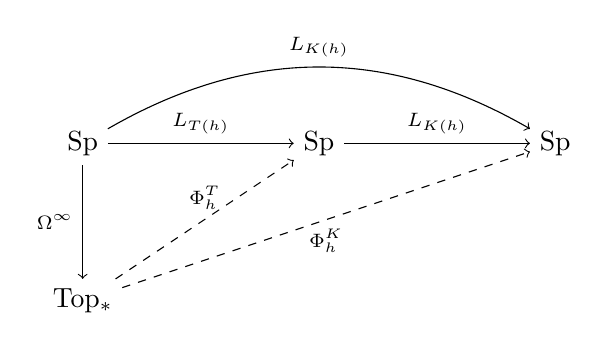
\begin{tikzpicture}
  \node (LT) at (0, 2) {Sp};
  \node (MT) at (3, 2) {Sp};
  \node (RT) at (6, 2) {Sp};
  \node (LB) at (0, 0) {Top$_*$};
  \draw [->] (LT) -- node [above] {$\scriptstyle L_{T(h)}$} (MT);
  \draw [->] (MT) -- node [above] {$\scriptstyle L_{K(h)}$} (RT);
  \draw [->] (LT) to [out = 30, in = 150] node [above] {$\scriptstyle L_{K(h)}$} (RT);
  \draw [->] (LT) -- node [left] {$\scriptstyle \Omega^\infty$} (LB);
  \draw [dashed,->] (LB) -- node [above] {$\scriptstyle \Phi^T_h$} (MT);
  \draw [dashed,->] (LB) -- node [below] {$\scriptstyle \Phi^K_h$} (RT);
 \end{tikzpicture}
\end{center}
Note that 
\[
 \begin{split}
  E^\wedge_*(\Phi^K_h X) = & ~ \pi_*(E \wedge \Phi^K_h X)_{K(h)} \\
                         = & ~ \pi_*(L_h \Phi^K_h X)_{K(h)} \\
                         = & ~ \pi_*(L_h L_{K(h)} \Phi^T_h X)_{K(h)} \\
                         = & ~ \pi_*(L_h \Phi^T_h X)_{K(h)} \\
                         = & ~ E^\wedge_*(\Phi^T_h X) 
 \end{split}
\]

\hskip .95cm $\Phi_h$ preserves fiber sequences (so do $\Omega^\infty$ and $L$) 

$\implies \Phi_h(\Omega Y) = \Omega \Phi_h(Y) \ce \Sigma^{-1} \Phi_h(Y)$ 

$\implies \Phi_h(X) \to \Phi_h(\Omega \Sigma X) = \Omega \Phi_h(\Sigma X)$ 

$\implies \Sigma \Phi_h(X) \to \Phi_h(\Sigma X)$ 

$\implies \Sigma^2 \Phi_h(X) \to \Phi_h(\Sigma^2 X)$ 

\underline{$h = 1$}
\begin{equation}
 \label{mooreseq}
 \Sigma^2 \Phi_1(S^{2 d + 1}) \to \Phi_1(S^{2 d + 3}) 
\end{equation}
Let $d = 4 n - 1$ and $p = 2$.  
Davis-Mahowald showed that, {\em $K(1)$-locally}, 
\[
 \bs^{-1} / 2^{4 n - 1} \simeq \bp_{1 - 8 n}^{-2} \qquad \ad \qquad \bs^{-1} / 2^{4 n} \simeq \bp_{1 - 8 n}^0 
\]
where $\bs^{-1} / m$ is the mod-$m$ Moore spectrum with $i$'th space $S^{i - 1} \cup_m e^i$, 
and $\bp_b^t = \Sigma^\infty \Sigma^b \BR\BP^{t - b}$ 
is the suspension spectrum of the stunted real projective space 
with top and bottom cells in dimensions $t$ and $b$.  
Thus in this case, in view of \eqref{BK1} and \eqref{Goode}, \eqref{mooreseq} becomes 
\[
 \bs_{K(1)}^{4 d + 3} / 2^d \to \bs_{K(1)}^{4 d + 3} / 2^{d + 1} 
\]
[Thu-7/21/16].  

Questions: 
\begin{itemize}
 \item Is this map multiplication by 2?  

 \item When $d = 4 n$, \eqref{mooreseq} becomes 
 \[
  \bs_{K(1)}^{4 d + 1} / 2^d \to \bs_{K(1)}^{4 d + 3} / 2^{d + 1} 
 \]
 When $d = 4 n + 1$, \eqref{mooreseq} becomes 
 \[
  \bs_{K(1)}^{4 d + 1} / 2^d \to \, ? 
 \]
 When $d = 4 n - 2$, \eqref{mooreseq} becomes 
 \[
  ? \to \bs_{K(1)}^{4 d + 5} / 2^{d + 1} 
 \]
 So $\Phi_1(S^{8 n - 3}) = \, ?$  
 Should there be a restriction on the result from [h2] at $p = 2$?  

 \item Is there an analog at odd primes?  
 Yes, at least for $p > 3$ [Davis], \eqref{mooreseq} becomes 
 \[
  \bs_{K(1)}^{2 d + 2} / p^d \to \bs_{K(1)}^{2 d + 2} / p^{d + 1} 
 \]

 \item How to ``stabilize'' this?  Cf [Arone-Mahowald, prop A.2(3)].  

 What is 
 \[
  \hocolim \Phi_1 S^{2 d + 1} 
 \]
 if each $\Phi_1 S^{2 d + 1}$ is $K(1)$-locally equivalent to (a suspension of) $\bm(p^d)$?  
 Cf [Arone-Mahowald, prop A.3] and note the difference.  

 \item Is there an analog $K(2)$-locally?  Be careful to distinguish $K(2)$ and $T(2)$.
\end{itemize}

The above process is related\footnote{Not quite the same.  
What is the relationship between the spectrum $\Phi_h S^q$ and the space $S^q_{K(h)}$?  
When $Y$ is an infinite loop space and $h = 1$, [Bousfield 82] shows that 
\[
 t\pi_2(Y_K) \cong t\pi_2(\Omega^\infty \Phi Y) \hskip 2cm \text{$t$ torsion subgroup} 
\]
\[
 \hskip -1.7cm \pi_i(Y_K) \cong \pi_i(\Omega^\infty \Phi Y) \hskip 2.2cm i \geq 3 
\]
So even when $Y$ is nice, the spaces $\Omega^\infty \Phi_h Y$ and $Y_{K(h)}$ are not the same.  
Cf [ulp, thm 5.6].  } 
to $K(1)$-localization and $v_1$-periodization of {\em unstable} spheres 
[Mahowald-Thompson], [Bousfield-loc/per], [ulp, \S\S 5-6].  
At height 2, these constructions become more complicated.  
Our calculation of $B_d$, through the lens of $E_2$-homology [email-7/7/16], 
might give some clue about how differently they behave.  

There are at least three related but different things going on here.  
Unstably, $\Phi_2(S^{2d+1})$ and $S^{2d+1}_{K(2)}$, 
$v_2$-periodic homotopy groups vs homotopy groups of the $K(2)$-localization, 
both completed at $p$.\footnote{Cf $h=1$: 
[Mahowald-Thompson, thm 1.2] (not true for an arbitrary space), 
where the telescope conjecture is true stably.  
Work at $h=2$: [Thompson-$L_2W(n)$].  }  
Stably, $\bs_{K(2)}$, $K(2)$-localization of the sphere {\em spectrum}.\footnote{Cf $h=1$: 
[Davis-Mahowald, Davis] studied {\em stable} $K(1)$-localization; 
[Mahowald-Thompson, thm 1.3] showed stable and unstable agree in high degrees.  }  

Understand $K(2)$-locally the spectra in \eqref{BK2} 
as well as layers of the Goodwillie tower in \eqref{Goode}, 
with starting point their $E$-homology discussed in [BKTAQ], 
indeed the source of our calculation.  


\subsection{Strict units}

[h2], [Sat-2/28/15], [Thu-Sem-4/3/14] (more?) 


\newpage
\section{[level3]}
\label{sec:level3}

- \textbf{Identifying the quantity we hope to be stable under the $K(1)$-local power operation $\psi$}

We have 
\[
 \pi_0 E_2 = {\mb Z}_9 \llbracket h \rrbracket,
\]
\[
 \pi_0 L_{K(1)} E_2 = {\mb Z}_9 (\!(h)\!)_3^\wedge.
\]
We want to show that the subring
\[
 {\mb Z}_9 \left[\frac{v_2}{v_1^4}\right]_3^\wedge \subset \pi_0 L_{K(1)} E_2
\]
is stable under the power operation 
\[
 \psi\co \pi_0 L_{K(1)} E_2 \to \pi_0 L_{K(1)} E_2,
\]
where $|v_1| = 2(3^1-1) = 4$ and $|v_2| = 2(3^2-1) = 16$.  
Note that as the generators of the homotopy of the generalized BP$\langle2\rangle$ spectrum, $v_1$ is only well-defined mod 3 and $v_2$ only mod $(3,v_1)$; 
different choices of these congruence classes may correspond to {\em different} formal group laws the graded ring $\BZ_{(3)}[v_1,v_2]$ carries 
(cf section 3 of [level3'] and [Fri-2/10/12]).

We need to make $v_2/v_1^4$ explicit. This amounts to a 3-primary analog of the last statement of proposition 5.4 on p29 of [level3] which is lemma 1 on p8 of [K(1)tmf]. 
Explicitly, given the equation of our elliptic curve
\[
 C \co y^2 + a x y + a c y = x^3 + c x^2
\]
with $|a| = 2$, $|c| = 4$, and
\[
 a_1 = a, \quad a_2 = c, \quad a_3 = a c, \quad a_4 = a_6 = 0,
\]
we have, using the formula on p188 of [Pearson2], 

$m_0 = 1$,

$m_1 = \frac{1}{3} (a_2 + a_1^2) = \frac{1}{3} (c + a^2)$,

$m_2 = \frac{1}{9} (a_2^4 + 6 a_4^2 + 12 a_4 a_2^2 + 15 a_1^4 a_2^2 + 10 a_2^3 a_1^2 + 12 a_2 a_6 + 42 a_3 a_1^5 + 7 a_1^6 a_2 + 90 a_3^2 a_1^2
 + 30 a_1^4 a_4 + 30 a_3^2 a_2 + 60 a_3 a_1 a_4 + 30 a_6 a_1^2 + 120 a_3 a_1^3 a_2 + 60 a_2^2 a_3 a_1 + 60 a_1^2 a_2 a_4 + a_1^8)
 = \frac{1}{9} (c^4 + 100 c^3 a^2 + 225 c^2 a^4 + 49 c a^6 + a^8)$,

where $m_i$ is the coefficient of $x^{3^i}$ in $\log_C(x)$. Given the relations
\[
 3 m_1 = m_0 v_1, \quad 3 m_2 = m_0 v_2 + m_1 v_1^3,
\]
we then have
\[
 v_1 = c + a^2,
\]
\[
 v_2 = 32 c^3 a^2 + 73 c^2 a^4 + 15 c a^6.
\]
\textcolor{red}{These use the coordinate $-x/y$ on $\HC$!  }

With the terminology in [level3'], our {\em (generalized) BP$\langle 2 \rangle$-realization problem} $(A,\BG)$ (definition 3.1 on p12) consists of
\[
 A = \BZ_{(3)}[v_1,v_2], \quad \BG = \widehat{C},
\]
and the {\em associated Lubin-Tate ring} (definition 4.1 on p19) is
\[
 B = \BZ_9 \llbracket u_1 \rrbracket [u^{\pm 1}].
\]
Writing
\[
 a = u t, \quad c = u^2, 
 \footnote{Adjust so ``\textcolor{red}{+}'' below? Change the equation of $C$ below accordingly? Jacobi quartic (Ravenel? Edwards?): $y^2 = x^4 + A x^3 + C, |A| = 2, |C| = 8$.  }
\]
$C$ is isomorphic to
\[
 y^2 + t x y + t y = x^3 + x^2
\]
with $h = u_1 = t^2 + 4$. The $A$-algebra structure on $B$ is then given by
\[
 v_1 \mapsto u^2 (u_1 - 3) \equiv u_1 u^2 \md 3,
\]
\[
 v_2 \mapsto u^8 (15 u_1^3 - 107 u_1^2 + 168 u_1 + 80) \equiv \textcolor{red}{-}\footnote{[Morava1207, 3.5]?}u^8 \md (3, u_1 u^2)
\]
({\em Is this reasonable?}).\\

\hrule

- (\texttt{h1p3\_alpha\_H\_-2.nb} and \texttt{closure.nb}) \textbf{Calculating $\psi(v_2 / v_1^4)$}

From above we have
\begin{eqnarray*}
 \frac{v_2}{v_1^4} & = & \frac{32 c^3 a^2 + 73 c^2 a^4 + 15 c a^6}{(c + a^2)^4} \\
                   & = & \frac{32 t^2 + 73 t^4 + 15 t^6}{(1 + t^2)^4} \\
                   & = & \frac{32 (h - 4) + 73 (h - 4)^2 + 15 (h - 4)^3}{(h - 3)^4} \\
                   & = & \frac{15}{H} + \frac{\textcolor{blue}{28}}{H^2} - \frac{69}{H^3} + \frac{\textcolor{blue}{26}}{H^4},
\end{eqnarray*}
where $H = h -3$. We then compute that
\[
 \psi(H) = H^3 - 27 H^2 + 183 H - 180 + \frac{186}{H} + \frac{1674}{H^2} + \cdots,
\]
and solve that
\[
 \psi(\frac{1}{H}) = \frac{1}{H^3} + \frac{27}{H^4} + \frac{546}{H^5} + \frac{9981}{H^6} + \frac{174243}{H^7} + \frac{2969622}{H^8} + \cdots,
\]
and thus
\[
 \psi(\frac{v_2}{v_1^4}) = \frac{15}{H^3} + \frac{405}{H^4} + \frac{8190}{H^5} + \frac{\textcolor{blue}{149743}}{H^6} + \frac{2615157}{H^7} + \frac{44595318}{H^8} + \cdots.
\]
Comparing the formulas of $v_2 / v_1^4$ and $\psi(v_2 / v_1^4)$, we conclude that the subring ${\mb Z}_9 [v_2 / v_1^4]_3^\wedge$ is not stable under $\psi$, 
as 15 is not invertible in $\BZ_9$ (the leading terms should match; cf 2/13/12 email).\\

\hrule

\textbf{Problem?} [6/20/13 email] 
\[
A = \BZ_{(3)} [a,c], \qquad \BG = \HC 
\]
but $A / (3,v_1,v_2) \not\cong \BF_3$ contradicts [level3', def 3.1].  

\textbf{Understand} what [level3] and [level3'] are doing.  
{\em There are more details to be worked out and it's not quite as straightforward as I may have hoped when writing level3, 
but I feel like it should be possible to figure out a lot about what kinds of schemes would have to carry p-divisible groups in order to make Jacob's machine work.  }

Perhaps the $\G_1(4)$ curve gives a non-example, and some other curve (Jacobi quartic?) gives an example, at the prime 3.  
{\em It seems unclear whether there is some 
isomorphism from this formal group law on $A$ to one coming from the 
smaller subring $\BZ_{(p)}[v_1,v_2] \subset A$ which has reasonable isogeny 
properties.  The same is true for most of the other modular curves.}  

So the machine in [level3] needs nice input data of specific formal group laws to work, 
even if we have some explicit calculations of power operations on Lubin-Tate spectra of height 2 at the prime 3.  
The paper [logetaletmf] should solve this realization problem in general (see the ``hope'' recorded on [level3, pp4-5]).  


\newpage
\section{Hecke operators}
\label{hecke}

\begin{itemize}
 \item Clarify the relationship between topological and classical Hecke operators [Sat-4/19/14] 
 and the relationship between homotopy groups of $E$-theory and rings of modular forms [\ref{subsubsec:kerlog} \eqref{padicmf}].  

 \item Kernel of the logarithm [4/22/14 email].  

 Logarithm detects ``genuine'' units?  (six conditions for meromorphic modular forms on $\G \subset \SL_2(\BZ)$ [Tue-1/27/15]) 

 [h2p2, exercise 2.9] 

 \item {[Sat-2/28/15 meeting]} appearance of $\vartheta$ and $\CE_2$:\footnote{\texttt{There are all kinds of areas where specific number theory formulas appear in physics, 
 and these may be clues that the dream will come true one day.  
 But to really get me excited, somehow the number theory would have to enter the physics in a more structural way.  
 I'm not that interested in a specific formula that comes out of a physics calculation in a more or less ad hoc fashion.  
 Number theory would have to be more integrated with the physics to get me excited, 
 and I don't see that happening soon.  }} Hodge extension ($\A$ and $h$), Gauss-Manin connection [padicprop, appendices; h2] 

 \item Does our vanishing result say something new/different about tmf orientations?  [koandtmf; Sprang] (Wilson) 
\end{itemize}


\texttt{It is notable that this expression from the theory of $L$-functions arises naturally from a purely topological construction; 
it came as a surprise to the author, 
and he still has no good explanation for it.  
It is also significant for the application to elliptic cohomology; 
in the presence of an elliptic curve, 
these Hecke operators coincide with the classical action of Hecke operators on modular forms.  }

$\MF(\BZ) = \BZ [c_4, c_6, \Delta, \Delta^{-1}] / (c_4^3 - c_6^2 = 1728 \Delta)$ 

\texttt{The key tool here is Rezk's $K(1)$-local logarithm, which permits a $K(1)$-local analysis of $Pic(Sp)$.  }

See also [koandtmf].  

\texttt{\href{http://www.math.northwestern.edu/~zyf/at/stable homotopy theory/Morava K-theories and infinite loop spaces.pdf}{The first paper}, 
an early application of the Nilpotence and Periodicity Theorems of Devinatz-Hopkins-Smith, 
exposed a curious relation between the stable and unstable worlds of homotopy, 
as viewed through the eyes of height n homology theories. 
My \\constructions, and Bousfield's more refined versions, 
seem to now be called Bousfield-Kuhn telescopic functors. 
Pete made much use of these ideas, 
and the telescopic functors underlie Rezk's `logarithmic' cohomology operations, 
and, in the case n = 2, were used in an essential way in the first announced proof 
by Hopkins and collaborators of the rigidification of the string bordism elliptic genus. }\\

$\displaystyle \D = q \prod_{n = 1}^\infty (1 - q^n)^{24} = \sum_{n = 1}^\infty \T(n) q^n = q - 24 q^2 + 252 q^3 - 1472 q^4 + 4830 q^5 + \cdots$ 

$\displaystyle \sum \T(n) n^{-s} = \prod (1 - \T(p) p^{-s} + p^{11 - 2s})^{-1}$ \hfill 
$\displaystyle \sum T(n) n^{-s} = \prod (1 - T(p) p^{-s} + T(p,p) p^{1 - 2s})^{-1}$ \\

\texttt{The modular variety $\CM_n$ is a smooth curve over $\BZ[1/n]$, 
whose ``physical appearance'' is the same whether we view it over $\BC$ 
(where it becomes $\phi(n)$ copies of the quotient of the upper half plane 
by the principal congruence subgroup $\G(n)$ of $\SL(2,\BZ)$) 
or over the algebraic closure of $\BZ / p \BZ$, 
(by ``reduction modulo $p$'') for primes $p$ not dividing $n$.  }

$j(z) = q^{-1} + 744 + 196884 q + \cdots$ 


\subsection{How Hecke operators act}

Cf [tmf3, proposition 5.2] (see also the normalizing factor $l^{k - 1} = \dfrac{1}{l} l^k$ in [Ka-22]).  
Note that they compute the $\G_1(3)$-curve under 3-isogeny, don't need a parameter for the universal example, 
and have $\psi^* \eta' = \eta$ (cf the construction in [tmf3, remark 5.4] and [dr, 4.38], see also [dr, remark 4.26]).  
$\todo$ Write down an analog of section 5 for $([\G_1(4)],[\G_0(3)])$?  Or something different?  For example, see \ref{subsubsec:h-opr} \eqref{moddscrp}.  

$\todo$ Read [tmf3] (in connection with [koandtmf], cited as [AHR], and with [prime2]).  

$\totodo$ All of these seem to have made an appearance in [K(1)E$_\infty$]; revisit and put these in context.  


\subsubsection{$h$-operators}
\label{subsubsec:h-opr}

$W(\K) = \K^{p + 1} + \cdots + (-H) \K + W_0 = 0$, $\psi^* du' = \K du$, $|\K| = -p + 1$, $\psi^* (\psi')^* du'' = \K \K' du = W_0 du$ 

$\displaystyle \l_n \ce \frac{1}{p} \sum_{i=0}^p \K_i^n$ \\
Note that $\l_1, \ldots, \l_{p+1}$ are related to the coefficients of $W(\K)$ via elementary symmetric functions 
and to our proposed dual basis for the \DL algebra (if we remove the \'etale part).  

$\G_1(3)$: $y^2 + a x y + b y = x^3$, $|a| = 1$, $|b| = 3$, $\Delta = b^3 (a^3 - 27 b)$ \\
$\d \ce a^3 - 27 b = (a - 3 b^{1/3}) (a^2 + 3 a b^{1/3} + 9 b^{2/3})$ \\
$a = 3, b = 1 \implies \d = 0$, abbreviated $\d \= 0$ 

$\G_1(4)$: $y^2 + a x y + a b y = x^3 + b x^2$, $|a| = 1$, $|b| = 2$, $\Delta = a^2 b^4 (a^2 - 16 b)$ \\
$a = 0, b = 1 \implies \D = 0$, abbreviated $\D \- 0$ \\
$\d \ce a^2 - 16 b = (a - 4 b^{1/2}) (a + 4 b^{1/2})$ \\
$a = \pm4, b = 1 \implies \d = 0$, abbreviated $\d \= 0$ 

The weighted projective space, the cusps: by abuse of notation, $V(\D) \supset V(\d) \subset D(a) \cap D(b)$.  

\begin{itemize}
 \item $\G_1(3)$ at 2 (\texttt{h2.nb}): $W(\K) = \K^3 - \dfrac{a}{b} \K - \dfrac{2}{b}$, \quad $H = \dfrac{a}{b}$ 

 $\l_1 = 0 = \si_0(2) - 2$ \hfill $\md 2$

 $\l_2 = \dfrac{a}{b} \= 3 = \si_1(2)$ \hfill $\l_2 = H$ 

 $\l_3 = \dfrac{3}{b} \= 3 = \si_2(2) - 2$ \hfill $\l_3 \equiv \dfrac{1}{b}$ 

 $\l_4 = \dfrac{a^2}{b^2} \= 9 = \si_3(2)$ \hfill $\l_4 \equiv H^2$ 

 $\l_5 = \dfrac{5 a}{b^2} \= 15 = \si_4(2) - 2$ \hfill $\l_5 \equiv \dfrac{H}{b}$ 

 $\l_6 = \dfrac{a^3 + 6 b}{b^3} \= 33 = \si_5(2)$ \hfill $\l_6 \equiv H^3$ 

 $\l_7 = \dfrac{7 a^2}{b^3} \= 63 = \si_6(2) - 2$ \hfill $\l_7 \equiv \dfrac{H^2}{b}$ 

 $\l_8 = \dfrac{a (a^3 + 16 b)}{b^4} \= 129 = \si_7(2)$ \hfill $\l_8 \equiv H^4$ 

 $\l_9 = \dfrac{3 (3 a^3 + 4 b)}{b^4} \= 255 = \si_8(2) - 2$ \hfill $\l_9 \equiv \dfrac{H^3}{b}$ 

 $\l_{10} = \dfrac{a^2 (a^3 + 30 b)}{b^5} \= 513 = \si_9(2)$ \hfill $\l_{10} \equiv H^5$ 

 $\l_{11} = \dfrac{11 a (a^3 + 4 b)}{b^5} \= 1023 = \si_{10}(2) - 2$ \hfill $\l_{11} \equiv \dfrac{H^4}{b}$ 

 $\l_{12} = \dfrac{a^6 + 48 a^3 b + 24 b^2}{b^6} \= 2049 = \si_{11}(2)$ \hfill $\l_{12} \equiv H^6$ 

 $\l_0 = \dfrac{3}{2} = \si_{-1}(2)$ 

 $\l_{-1} = -\dfrac{a}{4} \= -\dfrac{3}{4} = \si_{-2}(2) - 2$ 

 $\l_{-2} = \dfrac{a^2}{8} \= \dfrac{9}{8} = \si_{-3}(2)$ 

 $\l_{-3} = -\dfrac{a^3 - 12 b}{16} \= -\dfrac{15}{16} = \si_{-4}(2) - 2$ 

 $\l_{-4} = \dfrac{a (a^3 - 16 b)}{32} \= \dfrac{33}{32} = \si_{-5}(2)$ 

 $\l_{-5} = -\dfrac{a^2 (a^3 - 20 b)}{64} \= -\dfrac{63}{64} = \si_{-6}(2) - 2$ 

 $\l_{-6} = \dfrac{a^6 - 24 a^3 b + 48 b^2}{128} \= \dfrac{129}{128} = \si_{-7}(2)$ 

 \item $\G_1(4)$ at 3 (\texttt{h3.nb}): $W(\K) = \K^4 - \dfrac{6}{b^2} \K^2 + \dfrac{a^2 - 8 b}{b^4} \K - \dfrac{3}{b^4}$, \quad $H = -\dfrac{a^2 - 8 b}{b^4}$ 

 $\l_1 = 0 = -(\si_0(3) - 2)$ \hfill $\md 3$

 $\l_2 = \dfrac{4}{b^2} \= 4 = \si_1(3)$ \hfill $\l_2 \equiv \dfrac{1}{b^2}$ 

 $\l_3 = \dfrac{-a^2 + 8 b}{b^4} \= -8 = -(\si_2(3) - 2)$ \hfill $\l_3 = H$ 

 $\l_4 = \dfrac{28}{b^4} \= 28 = \si_3(3)$ \hfill $\l_4 \equiv \dfrac{1}{b^4}$ 

 $\l_5 = \dfrac{10 (-a^2 + 8 b)}{b^6} \= -80 = -(\si_4(3) - 2)$ \hfill $\l_5 \equiv \dfrac{H}{b^2}$ 

 $\l_6 = \dfrac{a^4 -16 a^2 b + 244 b^2}{b^8} \= 244 = \si_5(3)$ \hfill $\l_6 \equiv H^2$ 

 $\l_7 = \dfrac{91 (-a^2 + 8 b)}{b^8} \= -728 = -(\si_6(3) - 2)$ \hfill $\l_7 \equiv \dfrac{H}{b^4}$ 

 $\l_8 = \dfrac{4 (4 (a^4 - 16 a^2 b) + 547 b^2)}{b^{10}} \= 2188 = \si_7(3)$ \hfill $\l_8 \equiv \dfrac{H^2}{b^2}$ 

 $\l_9 = \dfrac{(-a^2 + 8 b) (a^4 - 16 a^2 b + 820 b^2)}{b^{12}} \= -6560 = -(\si_8(3) - 2)$ \hfill $\l_9 \equiv H^3$ 

 $\l_{10} = \dfrac{38 (5 (a^4 - 16 a^2 b) + 518 b^2)}{b^{12}} \= 19684 = \si_9(3)$ \hfill $\l_{10} \equiv \dfrac{H^2}{b^4}$ 

 $\l_{11} = \dfrac{11 (-a^2 + 8 b) (2 (a^4 - 16 a^2 b) + 671 b^2)}{b^{14}} \= -59048 = -(\si_{10}(3) - 2)$ \hfill $\l_{11} \equiv \dfrac{H^3}{b^2}$ 

 $\l_{12} = \dfrac{(a^4 - 16 a^2 b + 2072 b^2) (a^4 - 16 a^2 b) + 177148 b^4}{b^{16}} \= 177148 = \si_{11}(3)$ \hfill $\l_{12} \equiv H^4$ 

 $\l_0 = \dfrac{4}{3} = \si_{-1}(3)$ 

 $\l_{-1} = \dfrac{8 b - a^2}{-9} \= \dfrac{8}{9} = -(\si_{-2}(3) - 2)$ 

 $\l_{-2} = \dfrac{(-a^2 + 2 b) (-a^2 + 14 b)}{27} \= \dfrac{28}{27} = \si_{-3}(3)$ 

 $\l_{-3} = \dfrac{(-a^2 + 8 b) (a^4 - 16 a^2 b + 10 b^2)}{-81} \= \dfrac{80}{81} = -(\si_{-4}(3) - 2)$ 

 $\l_{-4} = \dfrac{a^8 - 32 a^6 b + 312 a^4 b^2 - 896 a^2 b^3 + 244 b^4}{243} \= \dfrac{244}{243} = \si_{-5}(3)$ 

 $\l_{-5} = -\dfrac{(-a^2 + 8 b) (a^8 - 32 a^6 b + 294 a^4 b^2 - 608 a^2 b^3 + 91 b^4)}{-729} \= \dfrac{728}{729} = -(\si_{-6}(3) - 2)$ 

 $\l_{-6} = \dfrac{a^{12} - 48 a^{10} b + 852 a^8 b^2 - 6784 a^6 b^3 + 23046 a^4 b^4 - 24672 a^2 b^5 + 2188 b^6}{2187} \= \dfrac{2188}{2187} = \si_{-7}(3)$ 

 \item $\G_1(3)$ at 5 (\texttt{h5\_3.nb}): $W(\K) = \K^6 - \dfrac{5 a}{b^3} \K^4 + \dfrac{40}{b^4} \K^3 - \dfrac{5 a^2}{b^6} \K^2 + \dfrac{a^4 - 19 a b}{b^8} \K - \dfrac{5}{b^8}$, 
 \quad $H = -\dfrac{a^4 - 19 a b}{b^8}$ 

 $\l_1 = 0 = -(\si_0(5) - 2)$ \hfill $\md 5$

 $\l_2 = \dfrac{2 a}{b^3} \= 6 = \si_1(5)$ \hfill $\l_2 \equiv \dfrac{2 a}{b^3}$ 

 $\l_3 = -\dfrac{24}{b^4} \= -24 = -(\si_2(5) - 2)$ \hfill $\l_3 \equiv \dfrac{1}{b^4}$ 

 $\l_4 = \dfrac{14 a^2}{b^6} \= 126 = \si_3(5)$ \hfill $\l_4 \equiv -\dfrac{a^2}{b^6}$ 

 $\l_5 = -\dfrac{a (a^3 + 181 b)}{b^8} \= -624 = -(\si_4(5) - 2)$ \hfill $\l_5 \equiv H$ 

 $\l_6 = \dfrac{2 (40 a^3 + 483 b)}{b^9} \= 3126 = \si_5(5)$ \hfill $\l_6 \equiv \dfrac{1}{b^8}$ 

 $\l_7 = -\dfrac{7 a^2 (a^3 + 221 b)}{b^{11}} \= -15624 = -(\si_6(5) - 2)$ \hfill $\l_7 \equiv \dfrac{2 a H}{b^3}$ 

 $\l_8 = \dfrac{2 a (267 a^3 + 5812 b)}{b^{12}} \= 78126 = \si_7(5)$ \hfill $\l_8 \equiv \dfrac{H}{b^4}$ 

 $\l_9 = -\dfrac{6 (9 a^6 + 1929 a^3 b + 6460 b^2)}{b^{14}} \= -390624 = -(\si_8(5) - 2)$ \hfill $\l_9 \equiv -\dfrac{a^2 H}{b^6}$ 

 $\l_{10} = \dfrac{a^2 (a^6 + 3512 a^3 b + 121461 b^2)}{b^{16}} \= 1953126 = \si_9(5)$ \hfill $\l_{10} \equiv H^2$ 

 $\l_{11} = -\dfrac{11 a (35 a^6 + 7856 a^3 b + 58301 b^2)}{b^{17}} \= -9765624 = -(\si_{10}(5) - 2)$ \hfill $\l_{11} \equiv \dfrac{H}{b^8}$ 

 $\l_{12} = \dfrac{2 (6 a^9 + 11902 a^6 b + 549696 a^3 b^2 + 777615 b^3)}{b^{19}} \= 48828126 = \si_{11}(5)$ \hfill $\l_{12} \equiv \dfrac{2 a H^2}{b^3}$ 

 $\l_0 = \dfrac{6}{5} = \si_{-1}(5)$ 

 $\l_{-1} = \dfrac{19 a b - a^4}{-25} \= \dfrac{24}{25} = -(\si_{-2}(5) - 2)$ 

 $\l_{-2} = \dfrac{(a^2 (a^6 - 38 a^3 b + 311 b^2)}{125} \= \dfrac{126}{125} = \si_{-3}(5)$ 

 $\l_{-3} = -\dfrac{a^{12} - 57 a^9 b + 1008 a^6 b^2 - 5434 a^3 b^3 + 3000 b^4}{-625} \= \dfrac{624}{625} = -(\si_{-4}(5) - 2)$ 

 $\l_{-4} = \dfrac{a (a^{15} - 76 a^{12} b + 2066 a^9 b^2 - 23636 a^6 b^3 + 99471 a^3 b^4 - 78500 b^5)}{3125} \= \dfrac{3126}{3125} = \si_{-5}(5)$ 

 $\l_{-5} = -\dfrac{a^2 (a^{18} - 95 a^{15} b + 3485 a^{12} b^2 - 61465 a^9 b^3 + 524355 a^6 b^4 - 1871224 a^3 b^5 + 1739375 b^6)}{-15625} \= \dfrac{15624}{15625} = -(\si_{-6}(5) - 2)$ 

 $\l_{-6} = (a^{24} - 114 a^{21} b + 5265 a^{18} b^2 - 125780 a^{15} b^3 + 1641540 a^{12} b^4 - 11300694 a^9 b^5 + 35837606 a^6 b^6 - 36714000 a^3 b^7 + 3018750 b^8) / 78125 
 \= \dfrac{78126}{78125} = \si_{-7}(5)$ 

 \item $\G_1(4)$ at 5 (\texttt{h5\_4.nb}): $W(\K) = \K^6 - \dfrac{10}{b^2} \K^5 + \dfrac{35}{b^4} \K^4 - \dfrac{60}{b^6} \K^3 + \dfrac{55}{b^8} \K^2 
 - \dfrac{a^4 - 16 a^2 b + 26 b^2}{b^{12}} \K ~\textcolor{red}{+}~ \dfrac{5}{b^{12}}$, 

 \hfill $H = \dfrac{a^4 - 16 a^2 b + 26 b^2}{b^{12}}$ 

 $\l_1 = \dfrac{2}{b^2} \= 2 = \si_0(5)$ \hfill $\md 5$

 $\l_2 = \dfrac{6}{b^4} \= 6 = \si_1(5)$ \hfill $\l_2 \equiv \dfrac{1}{b^4}$ 

 $\l_3 = \dfrac{26}{b^6} \= 26 = \si_2(5)$ \hfill $\l_3 \equiv \dfrac{1}{b^6}$ 

 $\l_4 = \dfrac{126}{b^8} \= 126 = \si_3(5)$ \hfill $\l_4 \equiv \dfrac{1}{b^8}$ 

 $\l_5 = \dfrac{a^4 - 16 a^2 b + 626 b^2}{b^{12}} \= 626 = \si_4(5)$ \hfill $\l_5 \equiv H$ 

 $\l_6 = \dfrac{6 (2 (a^4 - 16 a^2 b) + 521 b^2)}{b^{14}} \= 3126 = \si_5(5)$ \hfill $\l_6 \equiv \dfrac{2 a^4 - 2 a^2 b + b^2}{b^{14}}$ 

 $\l_7 = \dfrac{13 (7 (a^4 - 16 a^2 b) + 1202 b^2)}{b^{16}} \= 15626 = \si_6(5)$ \hfill $\l_7 \equiv \dfrac{H}{b^4}$ 

 $\l_8 = \dfrac{6 (96 (a^4 - 16 a^2 b) + 13021 b^2)}{b^{18}} \= 78126 = \si_7(5)$ \hfill $\l_8 \equiv \dfrac{H}{b^6}$ 

 $\l_9 = \dfrac{34 (99 (a^4 - 16 a^2 b) + 11489 b^2)}{b^{20}} \= 390626 = \si_8(5)$ \hfill $\l_9 \equiv \dfrac{H}{b^8}$ 

 $\l_{10} = \dfrac{(a^4 - 16 a^2 b + 18952 b^2) (a^4 - 16 a^2 b) + 1953126 b^4}{b^{24}} \= 1953126 = \si_9(5)$ \hfill $\l_{10} \equiv H^2$ 

 $\l_{11} = \dfrac{2 ((11 a^4 - 176 a^2 b + 52349 b^2) (a^4 - 16 a^2 b) + 4882813 b^4)}{b^{26}} \= 9765626 = \si_{10}(5)$ \\
 $\textcolor{white}{\l_{11}~\!} \equiv \dfrac{(2 a^4 - 2 a^2 b + b^2) H}{b^{14}} \md 5$ 

 $\l_{12} = \dfrac{138 ((2 a^4 - 32 a^2 b + 4144 b^2) (a^4 - 16 a^2 b) + 353827 b^4)}{b^{28}} \= 48828126 = \si_{11}(5)$ \\
 $\textcolor{white}{\l_{12}~\!} \equiv \dfrac{H^2}{b^4} \md 5$ 

 $\l_0 = \dfrac{6}{5} = \si_{-1}(5)$ 

 $\l_{-1} = \dfrac{a^4 - 16 a^2 b + 26 b^2}{25} \= \dfrac{26}{25} = \si_{-2}(5)$ 

 $\l_{-2} = \dfrac{a^8 - 32 a^6 b + 308 a^4 b^2 - 832 a^2 b^3 + 126 b^4}{125} \= \dfrac{126}{125} = \si_{-3}(5)$ 

 $\l_{-3} = \dfrac{a^{12} - 48 a^{10} b + 846 a^8 b^2 - 6592 a^6 b^3 + 21171 a^4 b^4 - 19248 a^2 b^5 + 626 b^6}{625} \= \dfrac{626}{625} = \si_{-4}(5)$ 

 $\l_{-4} = (a^{16} - 64 a^{14} b + 1640 a^{12} b^2 - 21376 a^{10} b^3 + 148364 a^8 b^4 - 520576 a^6 b^5 + 775840 a^4 b^6 - 305664 a^2 b^7 + 3126 b^8) / 3125 
 \= \dfrac{3126}{3125} = \si_{-5}(5)$ 

 $\l_{-5} = (a^{20} - 80 a^{18} b + 2690 a^{16} b^2 - 49280 a^{14} b^3 + 532745 a^{12} b^4 - 3436976 a^{10} b^5 + 12731370 a^8 b^6 - 24489280 a^6 b^7 
 + 19701190 a^4 b^8 - 3882080 a^2 b^9 + 15626 b^{10}) / 15625 \= \dfrac{15626}{15625} = \si_{-6}(5)$ 

 $\l_{-6} = (a^{24} - 96 a^{22} b + 3996 a^{20} b^2 - 94400 a^{18} b^3 + 1390890 a^{16} b^4 - 13224576 a^{14} b^5 + 81124856 a^{12} b^6 - 311746176 a^{10} b^7 
 + 703009815 a^8 b^8 - 822412000 a^6 b^9 + 391419096 a^4 b^{10} - 42458496 a^2 b^{11} + 78126 b^{12}) / 78125 \= \dfrac{78126}{78125} = \si_{-7}(5)$ 
\end{itemize}

\underline{Patterns}
\begin{itemize}
 \item 
 \[
  \l_n \= \left\{
  \begin{array}{ll}
   \si_{n-1}(p) & \qquad n~~\text{even} \\
   (-1)^p (\si_{n-1}(p) - 2) & \qquad n~~\text{odd} 
  \end{array}
  \right.
 \]
 if $\Frob^2 = [-p]$, and 
 \[
  \l_n \= \si_{n-1}(p) 
 \]
 if $\Frob^2 = [p]$.  

 \item For $\G_1(4)$ at 3, 
 \[
  \l_n \- \left\{
  \begin{array}{ll}
   \si_{n-1}(3) & \qquad n~~\text{even} \\
   \si_{n-1}(3) - 2 & \qquad n~~\text{odd} 
  \end{array}
  \right.
 \]
 differing from the $\=$ formula by a sign in the odd case.  

 For $\G_1(4)$ at 5, $\l_n \- \si_{n-1}(5)$, same as the $\=$ formula.  

 Same pattern for $h \=$ vs $h \-$.  

 \item $\l_{n+p} \equiv \l_n H \md p$ for $n > 1$ 
 as a result of $H = -W_1$ and $p | W_n$, $1 < n \leq p$.  

 ($H = -W_1 
 ~\raisebox{-1.2 pt}{$\=$} \hspace{-.14 in} \raisebox{1.2 pt}{$\=$}~ 
 1 \md p$, cf [ssingcong, theorem 1.2(1)].)  

 \item $(\pm p)^n p \l_{-n} \equiv h^n \md p$ 
 ($\pm$ depending on $\Frob^2 = [\pm p]$) for $n \geq 0$ 
 as a result of $\Ht_p \K = H$.  
\end{itemize}

\underline{Questions} 
\begin{enumerate}[(i)]
 \item \label{behave} Why do $\l_n$ specialize to those values 
 at the cusps (when $\D$ and its factors vanish)?  
 When they do, are they analogous to the $h$-operator computed in [tmf3, proposition 5.2]?  
 How do singular curves behave under $p$-isogenies?  
 Eg, $y^2 + a x y + a b y = x^3 + b x^2 \stackrel{\-}{\leadsto} y^2 = x^3 + x^2$.  
 $\todo$ More precisely, how does a lift of Frobenius over the supersingular locus restrict/extend to the cusps?  
 What is the effect on 1-forms?  It is like the identity plus multiplication by $p$.  
 See [KM, 10.13].  

 \item \label{factors} What can we say about the factors of $\D$?  
 Note that 
 \[
  \frac{\D}{a^3 - 27 b} = b^3 \qquad \ad \qquad [2]^* du = \frac{2}{(b^{1/3})^3} du 
 \]
 \[
  \frac{\D}{a^4 - 16 a^2 b} = b^4 \qquad \ad \qquad [3]^* du = \frac{3}{(b^{1/2})^8} du 
 \]
 \[
  b' = b^p 
 \]

 \item \label{moddscrp} Is there a modular description for this operator (without specialization), 
 analogous to $h \co \CM \to \CM, (C) \mapsto (C/C[3])$ in [tmf3]?  

 \item Are there geometric interpretations for the mod $p$ periodicities?  Likely to be related to $H = V^*$.  
 Help understand $\A^p$ vs $\A'$ ($V \A$ vs $F \A$?) in the Eichler-Shimura congruence?  
\end{enumerate}


\subsubsection{Hecke operators}
\label{subsubsec:Hecke-opr}

By abuse of notation, given a $\G_1(N)$-form $f_n$ of weight $n$, write 
\[
 f_n = f_n(C/S, du, P_0) \qquad \ad \qquad (f_n')_i = f_n \! \left( C_{S_{p,i}} / A_i, d\psi_i(u), \psi_i(P_0) \right) 
\]
$\displaystyle T_p ~ f_n \ce \frac{1}{p} \sum_{i=0}^p \K_i^n ~ (f_n')_i$ \qquad\qquad homogeneously additive, not multiplicative \\
$|f_n| = n$, $|\K_i| = -p + 1$, $|(f_n')_i| = p n$, so $T_p$ preserves weight: $n = (-p + 1) n + p n$.  

\begin{itemize}
 \item $\G_1(3)$ at 2 (\texttt{t2.nb}): $a' = a^2 + 3 b \K - a b \K^2$, $b' = b^2$ \\

 $\Delta = b^3 (a^3 - 27 b) = b^3 \d$ 

 $c_4 = a^4 - 24 a b = a (a^3 - 24 b) \= 9 = 3^2$ 

 $c_6 = -a^6 + 36 a^3 b - 216 b^2 \= 27 = 3^3$ 

 $h = a \= 3 = \si_2(2) - 2$ \\

 $T_2(h) = 0 = (\si_0(2) - 2) h$ 

 $T_2(a^2) = 3 a^2 = \si_1(2) a^2$ 

 $T_2(b) = 3 b = (\si_2(2) - 2) b$ 

 \hfill $a^3$ is not an eigenform, but $T_2(\d) = -3 (a^3 - 27 b) = -(\si_2(2) - 2) \d$ 

 $T_2(c_4) = 9 a (a^3 - 24 b) = \si_3(2) c_4$ 

 \hfill in fact $a^4$, $a b$ are both eigenforms\footnote{Note that ``eigenform'' usually means {\em simultaneous} eigenvector for all $T_n$ with $(n,N) = 1$; 
 not here, though.  } 

 $T_2(a^2 b) = 15 a^2 b = (\si_4(2) - 2) a^2 b$ 

 \hfill neither of $a^5$, $a c_4$ are eigenforms, but $T_2(a^2 \d) = -15 a^2 (a^3 - 27 b) = -(\si_4(2) - 2) a^2 \d$ 

 $T_2(c_6) = -33 (a^6 - 36 a^3 b + 216 b^2) = \si_5(2) c_6$ 

 \hfill none of $a^6$, $a^3 b$, $b^2$, $a^2 c_4$, $a^3 \d$, $\d^2$ are eigenforms, but $T_2(b \d) = -6 b (a^3 - 27 b) = -6 \d$ 

 ... 

 $T_2(\Delta) = -24 (a^3 - 27 b) b^3 = \T(2) \Delta$ \\

 \item $\G_1(4)$ at 3 (\texttt{t3.nb}): $a' = \dfrac{1}{a} (a^4 - 12 a^2 b + 12 b^2 + (-6 a^2 b^2 + 20 b^3) \K + 4 b^4 \K^2 + (a^2 b^4 - 4 b^5) \K^3)$, $b' = b^3$ \\

 $\Delta = a^2 b^4 (a^2 - 16 b) = a^2 b^4 \d$ 

 $c_4 = a^4 - 16 a^2 b + 16 b^2 \= 16 = 4^2$ \\
 $\wt{c_4 = a^4 - 16 a^2 b + 16 b^2} \- 16 = (-4)^2$ 

 $c_6 = -a^6 + 24 a^4 b - 120 a^2 b^2 - 64 b^3 = -(a^2 - 8 b) (a^4 - 16 a^2 b - 8 b^2) \= 64 = 4^3$ \\
 $\wt{c_6 = -a^6 + 24 a^4 b - 120 a^2 b^2 - 64 b^3 = -(a^2 - 8 b) (a^4 - 16 a^2 b - 8 b^2)} \- -64 = (-4)^3$ 

 $h = -(a^2 - 8 b) \= -8 = -(\si_2(3) - 2)$ \\
 $\wt{h = -(a^2 - 8 b)} \- 8 = \si_2(3) - 2$ \\

 $T_3(a) = 0 = -(\si_0(3) - 2) a$ 

 $T_3(h) = -4 (a^2 - 8 b) = \si_1(3) h$ 

 \hfill in fact $a^2$, $b$ are both eigenforms 

 $T_3(a b) = -8 a b = -(\si_2(3) - 2) a b$ 

 \hfill $a^3$ is not an eigenform, but $T_3(a \d) = 8 a (a^2 - 16 b) = (\si_2(3) - 2) a \d$ 

 $T_3(c_4) = 28 (a^4 - 16 a^2 b + 16 b^2) = \si_3(3) c_4$ 

 \hfill in fact $a^4$, $a^2 b$, $b^2$ are all eigenforms 

 $T_3(a^3 b + 4 a b^2) = -80 a b (a^2 + 4 b) =  -(\si_4(3) - 2) (a^3 b + 4 a b^2)$\footnote{This generates the subspace with eigenvalue $-80$ 
 of the space spanned by $a^5$, $a^3 b$, $a b^2$.  }

 \hfill none of $a^5$, $a^3 b$, $a b^2$, $a c_4$, $a^3 \d$, $a \d^2$ are eigenforms, but $T_3(a b \d) = 0$ 

 $T_3(c_6) = -244 (a^2 - 8 b) (a^4 - 16 a^2 b - 8 b^2) = \si_5(3) c_6$ 

 \hfill none of $a^6$, $a^4 b$, $a^2 b^2$, $b^3$, $a^2 c_4$, $b c_4$, $a^4 \d$, $b^2 \d$, $c_4 \d$, $a^2 \d^2$, $b \d^2$, $\d^3$ are eigenforms, 

 \hfill but $T_3(a^2 b \d) = -12 a^2 b \d$ 

 ... 

 $T_3(\Delta) = 252 a^2 (a^2 - 16 b) b^4 = \T(3) \Delta$ \\

 \item $\G_1(3)$ at 5 (\texttt{t5\_3.nb}): $a' = ?$, assume $b' = b^5$ \\

 $h = -(a^4 - 19 a b) \= -24 = -(\si_2(5) - 2)$ \\

 $T_5(b) = -24 b = -(\si_2(5) - 2) b$ \\

 \item $\G_1(4)$ at 5 (\texttt{t5\_4.nb}): $a' = ~\! ?$, assume $b' = b^5$, ungraded $h'$ known in \ref{formula5} 
 (can recover a graded formula by filling in powers of $b$ and changing $\A$ to $\K$) \\

 $h = a^4 - 16 a^2 b + 26 b^2 \= 26 = \si_2(5)$ \\
 $\wt{h = a^4 - 16 a^2 b + 26 b^2} \- 26 = \si_2(5)$ \\

 $T_5(b) = 6 b = \si_1(5) b$ 

 Calculate ungradedly: 

 $T_5(h) = 126 h = \si_3(5) h$ 

 $T_5(c_4) = 126 (-10 + h) = \si_3(5) c_4$ 

 $T_5(\Delta) = 4830 (-26 + h) = \T(5) \Delta$ 
\end{itemize}

\underline{Patterns and questions} 
\begin{enumerate}[(i)]
 \item The simultaneous eigenforms $E_4 = c_4$, $E_6 = -c_6$, $\D$ 
 have expected eigenvalues $\si_3(p)$, $\si_5(p)$, $\T(p)$.  

 Setting $b = 1$, we get an action of Hecke operators on $E$-theory, with $\K$ localized to $\A$.  
 [log, section 14] describes the action of $\BZ[T_{1,p}, \ldots, T_{n,p}]$ on $p^{-1} E^0 X$; 
 even better, we see here that $T_{1,p}$ actually acts on $E^0$ except for the scalars.  

 \item \label{oversing} The ``sporadic'' eigenvalues agree with $\l_n$.  
 In fact, more generally, for $\G_1(3)$, if $f_n$ is not divisible by $a - 3$ or $a^2 + 3 a + 9$, 
 \[
  T_p ~ f_n \= \l_n f_n; 
 \]
 for $\G_1(4)$, if $f_n$ is not divisible by $a - 4$ or $a + 4$, 
 \[
  T_p ~ f_n \= \l_n f_n, 
 \]
 and if $f_n$ is not divisible by $a$, 
 \[
  T_p ~ f_n \- \l_n f_n.  
 \]
 In these cases, it is as if at the cusps no $'$ is applied to $f_n$ in the definition of $T_p$; cf \ref{subsubsec:h-opr} \eqref{behave}.  
 This pattern is specific for the cusps and not true for an arbitrary point in the fundamental domain.  

 On the other hand, most of the forms divisible by factors of $\D$ exhibit ``new'' eigenvalues, including the expected $\T$-function for $\D$.  
 For example, 
 \begin{itemize}
  \item $\G_1(3)$ at 2 (\texttt{t2.nb}): $\l_{m,n} :\= T_2(a^m b^n \d) / (a^m b^n \d)$ \\
  \begin{tabular}{c|rrrr}
   $m + 3 n + 3$ & $n = 0$ & $n = 1$ & $n = 2$ & $n = 3$ \\
   3 & $-$3 & & & \\
   4 & 9 & & & \\
   5 & $-$15 & & & \\
   6 & {\em 21} & $-$6 & & \\
   7 & {\em $-$27} & 0 & & \\
   8 & {\em 33} & 6 & & \\
   9 & {\em $-$39} & {\em $-$12} & {\em 15} & \\
   10 & {\em 45} & 18 & {\em $-$9} & \\
   11 & {\em $-$51} & {\em $-$24} & {\em 3} & \\
   12 & {\em 57} & {\em 30} & {\em 3} & \rd{$-$24} 
  \end{tabular}
  \begin{equation*}
   \begin{split}
    \l_{m,n} = & ~ (-1)^{m + 3 n + 3} (3 + 6 (m + 3 n + 3 - 3)) + (-1)^{m + 3 n + 3 + 1} 27 n \\
             = & ~ 3 (-1)^{m + 3 n + 1} (2 m - 3 n + 1) 
   \end{split}
  \end{equation*}
  with $\l_{0,3} = \T(2)$ as $\D = b^3 \d$, and with $\l_{1,0} = \si_3(2) \= \l_4$ 

  $T_2(\d) = -3 \d$ 

  $T_2(\d^2) \= 729 \d = 3^6 \d$ 

  $T_2(\d^3) \= -6561 \d^2 = -3^8 \d^2$ 

  $T_2(\d^4) \= 531441 \d^2 = 3^{12} \d^2$ 

  \item $\G_1(4)$ at 3 (\texttt{t3.nb}): $\l_{m,n} :\= T_3(a^m b^n \d) / (a^m b^n \d)$ \\
  \begin{tabular}{c|rrrrrr}
   $m + 2 n + 2$ & $n = 0$ & $n = 1$ & $n = 2$ & $n = 3$ & $n = 4$ & $n = 5$ \\
   2 & 4 & & & & & \\
   3 & 8 & & & & & \\
   4 & 28 & 28 & & & & \\
   5 & {\em 64} & 0 & & & & \\
   6 & {\em 116} & $-$12 & {\em 116} & & & \\
   7 & {\em 184} & {\em $-$8} & {\em 56} & & & \\
   8 & {\em 268} & 12 & 12 & {\em 268} & & \\
   9 & {\em 368} & {\em 48} & {\em $-$16} & {\em 176} & & \\
   10 & {\em 484} & {\em 100} & {\em $-$28} & {\em 100} & {\em 484} & \\
   11 & {\em 616} & {\em 168} & {\em $-$24} & {\em 40} & {\em 360} & \\
   12 & {\em 764} & 252 & {\em $-$4} & {\em $-$4} & \rd{252} & {\em 764} 
  \end{tabular}
  \begin{equation*}
   \begin{split}
    \l_{m,n} = & ~ 4 + \frac{(4 + 4 + 16 (m + 2 n + 2 - 3)) (m + 2 n + 2 - 2)}{2} \\ 
               & + 64 \frac{(-(m + 2 n + 2 - 4) - (m + 2 n + 2 - 4) + 4 (n - 1)) n}{2} \\
             = & ~ 4 (2 m^2 - 8 m n + 8 n^2 - m - 2 n +1) \\
             = & ~ 4 (2 (m - 2 n)^2 - m - 2 n + 1) 
   \end{split}
  \end{equation*}
  with $\l_{2,4} = \T(3)$ as $\D = a^2 b^4 \d$, with $\l_{0,0} = \si_1(3) \= \l_2$, and with $\l_{2,0} = \l_{0,1} = \si_3(3) \= \l_4$ 

  $T_3(\d) = 4 \d$ 

  $T_3(\d^2) = 28 \d^2 = \si_3(3) \d^2$ 

  $T_3(\d^3) \= 65536 \d = 4^8 \d$ 

  $T_3(\d^4) \= 1048576 \d^2 = 4^{10} \d^2$ 
 \end{itemize}
 We can also examine, eg, $T_2((a - 3)^i (a^2 + 3 a + 9)^j)$ [Wed-8/6/14].  

 Are there functions (or coefficients in the $q$-expansions of certain modular forms) analogous to $\l_n$ that count for all these ``eigenvalues?''  

 Can we deduce some of the \href{http://en.wikipedia.org/wiki/Ramanujan_tau_function}{properties} of $\T$, 
 eg multiplicativity, from this viewpoint (of isogenies)?  
 We see $(p + 1) | \T(p)$.  

 Is there a more general theory for Hecke operators acting on {\em elliptic functions} 
 that specializes to give the expected eigenforms?  

 \item 
 \[
  h \= \left\{
  \begin{array}{ll}
   (-1)^p (\si_2(p) - 2) & \qquad \text{if ~ $\Frob^2 = [-p]$} \\
   \si_2(p) & \qquad \text{if ~ $\Frob^2 = [p]$} 
  \end{array}
  \right\} \equiv 1 \md p 
 \]
 the same formula for $\l_3$ (we also have $h \- \l_3$).  
 $c_4$ and $c_6$ also seem to specialize to powers of $N$.  

 Why?  Special values at the cusps?  

 \item \label{Tb} $b$ is an eigenform in all known cases: $\displaystyle T_p ~ b = \frac{1}{p} \sum \K_i^n b^p \= \l_n b$, ~ $|b| = n$ 

 $\displaystyle T_p ~ \K = \frac{1}{p} \sum \K_i^{-p+1} \K_i' = \frac{1}{p} \sum \K_i^{-p+1} \frac{W_0}{\K_i} = \l_{-p} W_0 = (\l_{-p} \K_1 \cdots \K_p) \K_0$, ~ $|\K| = -p + 1$ 
\end{enumerate}
 

\subsubsection{Hecke operators in terms of individual power operations}

$\displaystyle T_p(x) = \frac{1}{p} \sum_{i=0}^p \A_i^n \left( \sum_{j=0}^p Q_j(x) ~ \A_i^j \right)$ \quad for $x$ coming from a modular form of weight $n$ 

\begin{itemize}
 \item $\G_1(3)$ at 2 (\texttt{t2Q.nb}): 

 When $n = 0$, we have 
 \[
  T_2(x) = \dfrac{1}{2} (3 Q_0(x) + 2 a Q_2(x)) 
 \]

 Using relations from [h2p2], we compute that\footnote{The two identities in each pair agree when applied to $1$ (of weight 0), 
 given that $Q_0 \cdot 1 = 1$ and $Q_1 \cdot 1 = Q_2 \cdot 1 = 0$.  
 However, when applied to $a$ (of weight 1), they don't; 
 moreover, setting $n = 1$ for $T_2$, they do not either.  } 

 $Q_0 (3 Q_0 + 2 a Q_2) = 3 Q_0 Q_0 + 2 a^2 Q_0 Q_2 - 4 a Q_1 Q_2 + 12 Q_2 Q_2$ 

 $(3 Q_0 + 2 a Q_2) Q_0 = 3 Q_0 Q_0 + 2 a Q_0 Q_1 + 2 a^2 Q_0 Q_2 - 4 a Q_1 Q_2$ \\

 $Q_1 (3 Q_0 + 2 a Q_2) = 6 Q_2 Q_1 + 2 a Q_2 Q_2$ 

 $(3 Q_0 + 2 a Q_2) Q_1 = 3 Q_0 Q_1 + 2 a Q_2 Q_1$ \\

 $Q_2 (3 Q_0 + 2 a Q_2) = 3 Q_0 Q_1 + a Q_0 Q_2$ 

 $(3 Q_0 + 2 a Q_2) Q_2 = 3 Q_0 Q_2 + 2 a Q_2 Q_2$ 

 At height $n = 2$ and prime 2, we have $\Tt_{1,2} = 2 T_2$ and $\Tt_{2,2} = \Psi$,\footnote{In the notation of [Ka-22, 1.11.0.2], 
 \begin{equation*}
  \begin{split}
   (T_{2,\ell} ~ f) (E/R, \omega, \A_n) = & ~ \frac{1}{\ell^2} ~ \ell^k ~ f(E_{R'} / _\ell E_{R'}, \ell \omega, \ell \A_n) \\
                                        = & ~ \frac{1}{\ell^2} ~ f(E/R, \omega, \A_n) \\
                                        = & ~ \frac{1}{\ell^2} \Psi\!\left( f(E/R, \omega, \A_n) \right) 
  \end{split}
 \end{equation*}
 } 
 and $\Psi$ is in the center.\footnote{Since $\Psi = \psi^p \psi^p$ and $\psi^p = Q_0 + Q_1 \A + \cdots + Q_p \A^p$, 
 we can write $\psi^p \psi^p \psi^p$ as either 
 \[
  \Psi (Q_0 + Q_1 \A + \cdots + Q_p \A^p) = \Psi Q_0 + (\Psi Q_1) (\Psi \A) + \cdots + (\Psi Q_p) (\Psi \A)^p = \Psi Q_0 + (\Psi Q_1) \A + \cdots + (\Psi Q_p) \A^p 
 \]
 or 
 \[
  (Q_0 + Q_1 \A + \cdots + Q_p \A^p) \Psi = Q_0 \Psi + (Q_1 \Psi) \A + \cdots + (Q_p \Psi) \A^p 
 \]}  \\
 \underline{Question} \quad
 What is the center of $\G$?  See [8/28/14 email] and \eqref{center}.  
 (What is the center of $\CA$?)  \\

 For $n > 0$, we compute that 

 $T_2 = a Q_1 + 3 Q_2$ \hfill $n = 1$ 

 $T_2 = a Q_0 + 3 Q_1 + a^2 Q_2$ \hfill $n = 2$ 

 $T_2 = 3 Q_0 + a^2 Q_1 + 5 a Q_2$ \hfill $n = 3$ 

 $T_2 = a^2 Q_0 + 5 a Q_1 + (a^3 + 6) Q_2$ \hfill $n = 4$ 

 $T_2 = 5 a Q_0 + (a^3 + 6) Q_1 + 7 a^2 Q_2$ \hfill $n = 5$ 

 $T_2 = (a^3 + 6) Q_0 + 7 a^2 Q_1 + (a^4 + 16 a) Q_2$ \hfill $n = 6$ 

 $T_2 = 7 a^2 Q_0 + (a^4 + 16 a) Q_1 + (9 a^3 + 12) Q_2$ \hfill $n = 7$ 

 $T_2 = (a^4 + 16 a) Q_0 + (9 a^3 + 12) Q_1 + (a^5 + 30 a^2) Q_2$ \hfill $n = 8$ 

 $T_2 = (9 a^3 + 12) Q_0 + (a^5 + 30 a^2) Q_1 + (11 a^4 + 44 a) Q_2$ \hfill $n = 9$ 

 $T_2 = (a^5 + 30 a^2) Q_0 + (11 a^4 + 44 a) Q_1 + (a^6 + 48 a^3 + 24) Q_2$ \hfill $n = 10$ 

 $T_2 = (11 a^4 + 44 a) Q_0 + (a^6 + 48 a^3 + 24) Q_1 + (13 a^5 + 104 a^2) Q_2$ \hfill $n = 11$ 

 $T_2 = (a^6 + 48 a^3 + 24) Q_0 + (13 a^5 + 104 a^2) Q_1 + (a^7 + 70 a^4 + 112 a) Q_2$ \hfill $n = 12$ 

 Note the integrality, left-shifting, and mod 2 periodicity of the coefficients as $n$ increases.  
 These coefficients encode $W_i$ but not $W_i'$.  

 \item $\G_1(4)$ at 3 (\texttt{t3Q.nb}) 
\end{itemize}


\subsubsection{$q$-operators}

$\displaystyle \Ht_p ~ f_n \ce \sum_{i=0}^p (f_n')_i $ \qquad\qquad additive, not multiplicative 

$\Ht_p ~ f_n \equiv f_n^p \md p$ \\
Frobenius congruence for $(f_n')_0$ combined with integrality of $\l_1$, \ldots, $\l_p$, 
or, $\K_0 (\K_i^p - H) \equiv 0 \md p$, $1 \leq i \leq p$ 

$\Ht_p ~ \K = H$ \\
see section \ref{new} 

\underline{Motivation} \quad
In view of the definitions 
\[
 \l_n \ce \frac{1}{p} \sum_{i=0}^p \K_i^n \qquad T_p ~ f_n \ce \frac{1}{p} \sum_{i=0}^p \K_i^n ~ (f_n')_i \qquad \Ht_p ~ f_n \ce \sum_{i=0}^p (f_n')_i 
\]
we want to compare 
\[
 T_p ~ f_n \qquad \ad \qquad \l_n \cdot \Ht_p ~ f_n 
\]

Define the {\em ramification number} of $f_n$ (at cusps) 
\[
 r_p(f_n) \ce \left. \frac{\Ht_p ~ f_n}{(p + 1) ~ \widetilde{f}_n} \right|_\text{$a = 3$ (or 0, $\pm 4$) and $b = 1$} 
\]
where $\widetilde{f}_n$ is $f_n$ dividing all but one of its factors $a - 3$ (or $a$, $a \mp 4$) if they exist and $r_p$ is evaluated there.  

\underline{Patterns}
\begin{itemize}
 \item We have $r_p(f_n) = 1$ if $f_n$ is {\em relatively nonsingular} (does not contain $a - s$ when $r_p$ is evaluated at $s$).  In other words, 
 \[
  \Ht_p ~ f_n \= (p + 1) f_n 
 \]
 \rd{(explained in [Tue-10/7/14 meeting])} and thus 
 \[
  \l_n \cdot \Ht_p ~ f_n \= (p + 1) \l_n f_n 
 \]
 On the other hand, from \ref{subsubsec:Hecke-opr} \eqref{oversing} we have 
 \[
  T_p ~ f_n \= \l_n f_n 
 \]
 Note that the factor $a^2 + 3 a + 9$ does not play a special role for $\Ht_p$ as previously for $T_p$.  

 \item For $f_n$ relatively singular, we have, for example, 

 $r_2(\d) = 2 \cdot 4 = r_2(b \d) = r_2(b^3 \d = \D)$ 

 $r_2(a \d) = 2 \cdot 7$ 

 $r_2(a^2 \d) = 2 \cdot 10$ 

 $r_2(a^3 \d) = 2 \cdot 13$ 

 $r_2(\d^2) = 2 \cdot 3^5$ \\

 $r_3(\d) = 3 \cdot 11 = r_3(b \d) = r_3(b^2 \d)$ 

 $r_3(a \d) = 3 \cdot 35 = r_3(a b \d)$ 

 $r_3(a^2 \d) = 3 \cdot 75 = r_3(a^2 b \d) = r_3(a^2 b^4 \d = \D)$ 

 $r_3(a^3 \d) = 3 \cdot 131$ 

 $r_3(a^4 \d) = 3 \cdot 203$ 

 $r_3(c_4 \d) = 3 \cdot 2059$ 

 $r_3(\d^2) = 3 \cdot 4^4 \cdot 4 = r_3(b \d^2)$ 

 $r_3(a \d^2) = 3 \cdot 4^4 \cdot 6$ 

 $r_3(a^2 \d^2) = 3 \cdot 4^4 \cdot 8$ 

 $r_3(\d^3) = 3 \cdot 4^7$ 

 Cf \ref{subsubsec:Hecke-opr} \eqref{oversing}; note the (in)dependency on powers of $b$.  

 The correct (as opposed to simply ``$\l_n$'') eigenvalue 
 \[
  \frac{T_p ~ f_n}{f_n} = \frac{(p + 1) \frac{\Ht_p(f_n)}{(p + 1) f_n}}{\frac{\Ht_p(f_n)}{T_p(f_n)}} \= \frac{(p + 1) r_p(f_n) / (\text{singular factors})}{\Ht_p(f_n) / T_p(f_n)} 
 \]
 In particular 
 \[
  \T(p) \= \frac{(p + 1) r_p(\D)}{\Ht_p(\D) / T_p(\D)} 
 \]
\end{itemize}

\underline{Questions} 
\begin{itemize}
 \item How to interpret $r_p$ and its patterns?  Is ``ramification'' proper?  
 Behavior at the cusps?  \ref{subsubsec:h-opr} \eqref{behave}, \ref{subsubsec:Hecke-opr} \eqref{oversing}.  
\end{itemize}
 
\begin{itemize}
 \item $\G_1(3)$ at 2 (\texttt{q2.nb}): 

 $\Ht_2(a) = a^2 \= 3 a$ \\

 $\Ht_2(a^2) = a (a^3 - 18 b) \= 3 a^2$ \\

 $\Ht_2(a^3) = a^6 - 30 a^3 b + 162 b^2 \= 3 a^3$ 

 $\Ht_2(b) = 3 b^2 \= 3 b$ 

 $\Ht_2(\d) = (a^3 - 27 b) (a^3 - 3 b) \= 3 \cdot 2 \cdot 4 \d$ \\

 $\Ht_2(a^4) = a^2 (a^6 - 40 a^3 b + 378 b^2) \= 3 a^4$ 

 $\Ht_2(a b) = a^2 b^2 \= 3 a b$ 

 $\Ht_2(c_4) = a^2 (a^6 - 40 a^3 b + 354 b^2) \= 3 c_4$ 

 $\Ht_2(a \d) = a^2 (a^3 - 27 b) (a^3 - 13 b) \= 3 \cdot 2 \cdot 7 a \d$ \\

 $\Ht_2(a^5) = a (a^9 - 50 a^6 b + 720 a^3 b^2 - 2430 b^3) \= 3 a^5$ 

 $\Ht_2(a^2 b) = a (a^3 - 18 b) b^2 \= 3 a^2 b$ 

 $\Ht_2(a c_4) = a (a^9 - 50 a^6 b + 696 a^3 b^2 - 1998 b^3) \= 3 a c_4$ 

 $\Ht_2(a^2 \d) = a (a^3 - 27 b) (a^6 - 23 a^3 b + 72 b^2) \= 3 \cdot 2 \cdot 10 a^2 \d$ \\

 $\Ht_2(a^6) = a^{12} - 60 a^9 b + 1164 a^6 b^2 - 7614 a^3 b^3 + 8748 b^4 \= 3 a^6$ 

 $\Ht_2(a^3 b) = b^2 (a^6 - 30 a^3 b + 162 b^2) \= 3 a^3 b$ 

 $\Ht_2(b^2) = 3 b^4 \= 3 b^2$ 

 $\Ht_2(c_6) = -a^{12} + 60 a^9 b - 1128 a^6 b^2 + 6534 a^3 b^3 - 3564 b^4 \= 3 c_6$ 

 $\Ht_2(a^2 c_4) = a^{12} - 60 a^9 b + 1140 a^6 b^2 - 6894 a^3 b^3 + 4860 b^4 \= 3 a^2 c_4$ 

 $\Ht_2(a^3 \d) = (a^3 - 27 b) (a^9 - 33 a^6 b + 246 a^3 b^2 - 162 b^3) \= 3 \cdot 2 \cdot 13 a^3 \d$ 

 $\Ht_2(b \d) = (a^3 - 27 b) (a^3 - 3 b) b^2 \= 3 \cdot 2 \cdot 4 b \d$ 

 $\Ht_2(\d^2) = (a^3 - 27 b) (a^9 - 33 a^6 b + 219 a^3 b^2 - 81 b^3) = 3 \cdot 2 \cdot 3^5 \d$ \\

 ... \\

 $\Ht_2(\D) = (a^3 - 27 b) (a^3 - 3 b) b^6 \= 3 \cdot 2 \cdot 4 \D$ 

 $\Ht_2(a^{12}) = a^{24} - 120 a^{21} b + 5928 a^{18} b^2 - 154912 a^{15} b^3 + 
 2285040 a^{12} b^4 - 18703872 a^9 b^5 + 76855554 a^6 b^6 - 
 120932352 a^3 b^7 + 25509168 b^8 \= 3 a^{12}$ \\

 \item $\G_1(4)$ at 3 (\texttt{q3.nb}): 

 $\Ht_3(a) = a (a^2 - 12 b) \= 4 a$ \\

 $\Ht_3(a^2) = a^2 (a^4 - 24 a^2 b + 132 b^2) \= 4 a^2$ 

 $\Ht_3(b) = 4 b^3 \= 4 b$ 

 $\Ht_3(h) = -(a^2 - 8 b) (a^4 - 16 a^2 b + 4 b^2) \= 4 h$ 

 $\Ht_3(\d) = (a^2 - 16 b) (a^4 - 8 a^2 b + 4 b^2) \= 4 \cdot 3 \cdot 11 \d$ \\

 $\Ht_3(a^3) = a (a^8 - 36 a^6 b + 414 a^4 b^2 - 1548 a^2 b^3 + 768 b^4) \= 4 a^3$ 

 $\Ht_3(a b) = a (a^2 - 12 b) b^3 \= 4 a b$ 

 $\Ht_3(a \d) = a (a^2 - 16 b) (a^2 - 6 b) (a^4 - 14 a^2 b + 10 b^2) \= 4 \cdot 3 \cdot 35 a \d$ \\

 $\Ht_3(a^4) = a^2 (a^{10} - 48 a^8 b + 840 a^6 b^2 - 6384 a^4 b^3 + 18948 a^2 b^4 - 12288 b^5) \= 4 a^4$ 

 $\Ht_3(a^2 b) = a^2 b^3 (a^4 - 24 a^2 b + 132 b^2) \= 4 a^2 b$ 

 $\Ht_3(b^2) = 4 b^6 \= 4 b^2$ 

 $\Ht_3(c_4) = (a^4 - 16 a^2 b + 16 b^2) (a^8 - 32 a^6 b + 312 a^4 b^2 - 896 a^2 b^3 + 4 b^4) \= 4 c_4$ 

 $\Ht_3(a^2 \d) = a^2 (a^2 - 16 b) (a^8 - 32 a^6 b + 328 a^4 b^2 - 1152 a^2 b^3 + 
   900 b^4) \= 4 \cdot 3 \cdot 75 a^2 \d$ 

 $\Ht_3(b \d) = (a^2 - 16 b) b^3 (a^4 - 8 a^2 b + 4 b^2) \= 4 \cdot 3 \cdot 11 b \d$ 

 $\Ht_3(\d^2) = (a^2 - 16 b) (a^{10} - 32 a^8 b + 328 a^6 b^2 - 1168 a^4 b^3 + 
   1028 a^2 b^4 - 64 b^5) \= 4 \cdot 3 \cdot 4^4 \cdot 4 \d$ \\

 $\Ht_3(a^5) = a^3 (a^{12} - 60 a^{10} b + 1410 a^8 b^2 - 16260 a^6 b^3 + 
   93615 a^4 b^4 - 238092 a^2 b^5 + 176640 b^6) \= 4 a^5$ 

 $\Ht_3(a^3 b) = a b^3 (a^8 - 36 a^6 b + 414 a^4 b^2 - 1548 a^2 b^3 + 768 b^4) \= 4 a^3 b$ 

 $\Ht_3(a b^2) = a (a^2 - 12 b) b^6 \= 4 a b^2$ 

 $\Ht_3(a^3 b + 4 a b^2) = a b^3 (a^8 - 36 a^6 b + 414 a^4 b^2 - 1544 a^2 b^3 + 720 b^4) \= 4 (a^3 b + 4 a b^2)$ 

 $\Ht_3(a c_4) = a (a^{14} - 60 a^{12} b + 1410 a^{10} b^2 - 16276 a^8 b^3 + 94191 a^6 b^4 - 
   244716 a^4 b^5 + 201424 a^2 b^6 - 12480 b^7) \= 4 a c_4$ 

 $\Ht_3(a^3 \d) = a (a^2 - 16 b) (a^{12} - 44 a^{10} b + 706 a^8 b^2 - 4980 a^6 b^3 + 
   14511 a^4 b^4 - 12540 a^2 b^5 + 768 b^6) \= 4 \cdot 3 \cdot 131 a^3 \d$ 

 $\Ht_3(a b \d) = a (a^2 - 16 b) (a^2 - 6 b) b^3 (a^4 - 14 a^2 b + 10 b^2) \= 4 \cdot 3 \cdot 35 a b \d$ 

 $\Ht_3(a \d^2) = a (a^2 - 16 b) (a^{12} - 44 a^{10} b + 706 a^8 b^2 - 4996 a^6 b^3 + 
   14831 a^4 b^4 - 14044 a^2 b^5 + 1728 b^6) \= 4 \cdot 3 \cdot 4^4 \cdot 6 a \d$ \\

 $\Ht_3(a^6) = a^2 (a^{16} - 72 a^{14} b + 2124 a^{12} b^2 - 32904 a^{10} b^3 + 
   284382 a^8 b^4 - 1337328 a^6 b^5 + 3044484 a^4 b^6 - 
   2451456 a^2 b^7 + 196608 b^8) \= 4 a^6$ 

 $\Ht_3(a^4 b) = a^2 b^3 (a^{10} - 48 a^8 b + 840 a^6 b^2 - 6384 a^4 b^3 + 
   18948 a^2 b^4 - 12288 b^5) \= 4 a^4 b$ 

 $\Ht_3(a^2 b^2) = a^2 b^6 (a^4 - 24 a^2 b + 132 b^2) \= 4 a^2 b^2$ 

 $\Ht_3(b^3) = 4 b^9 \= 4 b^3$ 

 $\Ht_3(c_6) = -(a^2 - 8 b) (a^{16} - 64 a^{14} b + 1612 a^{12} b^2 - 20032 a^{10} b^3 + 125278 a^8 b^4 - 355264 a^6 b^5 + 355708 a^4 b^6 - 63424 a^2 b^7 - 32 b^8) 
 \= 4 c_6$ 

 $\Ht_3(a^2 c_4) = a^2 (a^{16} - 72 a^{14} b + 2124 a^{12} b^2 - 32920 a^{10} b^3 + 
   285150 a^8 b^4 - 1350768 a^6 b^5 + 3146644 a^4 b^6 - 
   2755008 a^2 b^7 + 395328 b^8) \= 4 a^2 c_4$ 

 $\Ht_3(b c_4) = b^3 (a^4 - 16 a^2 b + 16 b^2) (a^8 - 32 a^6 b + 312 a^4 b^2 - 
   896 a^2 b^3 + 4 b^4) \= 4 b c_4$ 

 $\Ht_3(a^4 \d) = a^2 (a^2 - 16 b) (a^{14} - 56 a^{12} b + 1228 a^{10} b^2 - 13272 a^8 b^3 + 
   72798 a^6 b^4 - 186000 a^4 b^5 + 170628 a^2 b^6 - 24576 b^7) \= 4 \cdot 3 \cdot 203 a^4 \d$ 

 $\Ht_3(a^2 b \d) = a^2 (a^2 - 16 b) b^3 (a^8 - 32 a^6 b + 328 a^4 b^2 - 1152 a^2 b^3 + 
   900 b^4) \= 4 \cdot 3 \cdot 75 a^2 b \d$ 

 $\Ht_3(b^2 \d) = (a^2 - 16 b) b^6 (a^4 - 8 a^2 b + 4 b^2) \= 4 \cdot 3 \cdot 11 b^2 \d$ 

 $\Ht_3(c_4 \d) = (a^2 - 16 b) (a^{16} - 56 a^{14} b + 1228 a^{12} b^2 - 13288 a^{10} b^3 + 
   73310 a^8 b^4 - 191248 a^6 b^5 + 189076 a^4 b^6 - 39104 a^2 b^7 + 
   64 b^8) \= 4 \cdot 3 \cdot 2059 c_4 \d$ 

 $\Ht_3(a^2 \d^2) = a^2 (a^2 - 16 b) (a^{14} - 56 a^{12} b + 1228 a^{10} b^2 - 13288 a^8 b^3 + 
   73310 a^6 b^4 - 191248 a^4 b^5 + 189060 a^2 b^6 - 38976 b^7) \= 4 \cdot 3 \cdot 4^4 \cdot 8 a^2 \d$ 

 $\Ht_3(b \d^2) = (a^2 - 16 b) b^3 (a^{10} - 32 a^8 b + 328 a^6 b^2 - 1168 a^4 b^3 + 
   1028 a^2 b^4 - 64 b^5) \= 4 \cdot 3 \cdot 4^4 \cdot 4 b \d$ 

 $\Ht_3(\d^3) = (a^2 - 16 b) (a^{16} - 56 a^{14} b + 1228 a^{12} b^2 - 13304 a^{10} b^3 + 
   73822 a^8 b^4 - 196496 a^6 b^5 + 207748 a^4 b^6 - 55424 a^2 b^7 + 
   1024 b^8) \= 4 \cdot 3 \cdot 4^7 \d$ \\

 ... \\

 $\Ht_3(\D) = a^2 (a^2 - 16 b) b^{12} (a^8 - 32 a^6 b + 328 a^4 b^2 - 1152 a^2 b^3 + 900 b^4) \= 4 \cdot 3 \cdot 75 \D$ 

 $\Ht_3(a^{12}) = a^4 (a^{32} - 144 a^{30} b + 9432 a^{28} b^2 - 371664 a^{26} b^3 + 
   9818316 a^{24} b^4 - 183401856 a^{22} b^5 + 2489392152 a^{20} b^6 - 
   24838888608 a^{18} b^7 + 182166373854 a^{16} b^8 - 
   971417530656 a^{14} b^9 + 3682200368592 a^{12} b^{10} - 
   9550209884976 a^{10} b^{11} + 15938000886276 a^8 b^{12} - 
   15458887987200 a^6 b^{13} + 7251602964480 a^4 b^{14} - 
   1104075030528 a^2 b^{15} + 12884901888 b^{16}) \= 4 a^{12}$ \\

 \item $\G_1(4)$ at 5 (\texttt{q5\_4.nb}): 

 $\Ht_5(h) = -3178240 + 267430 h + 18440 h^2 - 1340 h^3 - 10 h^4 + h^5 \= 6 h$ 

 $\Ht_5(c_4) = (-10 + h) (317830 + 5040 h - 1340 h^2 + h^4) \= 6 c_4$ 

 $\Ht_5(\D) = (-26 + h) (122246 - 5584 h - 924 h^2 + 16 h^3 + h^4) \= 6 \cdot 5 \cdot 3021 \D$ 
\end{itemize}


\subsection{Logarithms}
\label{subsec:log}

$l_{n,p} \co gl_1 E \to L_{K(n)} gl_1 E \simeq \Phi_n \Omega^\infty gl_1 E 
\simeq\footnote{Basepoint shifting, ``highly nontrivial.''  } 
\Phi_n \Omega^\infty E \simeq L_{K(n)} E = E^\wedge$ 

$l_{2,p} \co (E^0)^\times \to E^0$, \quad $\displaystyle l_{2,p}(x) = \sum_{k=1}^\infty (-1)^{k-1} \frac{p^{k-1}}{k} M(x)^k = \frac{1}{p} \log(1 + p M(x))$ 
\begin{equation*}
\begin{split}
 1 + p M(x) = & ~ \prod_{j=0}^2 \prod_{A \subset (\BQ_p/\BZ_p)^2 [p], |A| = p^j} \psi_A(x)^{(-1)^j p^{(j-1)(j-2)/2}} \\
            = & ~ x^p \cdot \frac{1}{\psi^p(x;\A_0) \cdots \psi^p(x;\A_p)} \cdot \Psi(x) \\
            = & ~ \frac{x^{p+1}}{\psi^p(x;\A_0) \cdots \psi^p(x;\A_p)} \qquad\qquad\qquad\qquad \text{multiplicative, not additive, sends (nonzero) scalars to 1} 
\end{split}
\end{equation*}
To be compatible with the action of Hecke operators in \ref{subsubsec:Hecke-opr}, 
the $2n$-graded version goes as\footnote{Be careful about the sign $(-1)^{p n}$; it won't be there if 
$[p]^* du = \K_0 \cdots \K_p \cdot du$ (true for $p = 2$), for which we do have a unique choice of coordinate (see [dr, remark 4.24]).  
We need $[p]$ for $\Psi$ because $p T_{2,p} = T_p T_p - T_{p^2}$ and on an eigenform this should give $p \dfrac{1}{p^2} p^n = \si_{n-1}(p)^2 - \si_{n-1}(p^2)$.  
Also, remember that for $\G_1(4)$ at 5 we just need $W_0^n$ so a sign won't appear.  
Perhaps we could say that $\psi^p(f_n)$ is more canonical than $f_n'$?  } 
\begin{equation}
\label{M}
\begin{split}
 1 + p M(f_n) = & ~ f_n^p \cdot \frac{1}{\K_0^n (f_n')_0 \cdots \K_p^n (f_n')_p} \cdot (-W_0)^n f_n b^{(p^2 n - n) / |b|} \\
              = & ~ f_n^p \cdot \frac{1}{((-1)^{p+1} W_0)^n (f_n')_0 \cdots (f_n')_p} \cdot (-W_0)^n f_n b^{(p^2 n - n) / |b|} \\
              = & ~ \frac{(-1)^{p n} f_n^{p+1} b^{(p^2 n - n) / |b|}}{(f_n')_0 \cdots (f_n')_p} \qquad\qquad\qquad\qquad\qquad\qquad\qquad \text{multiplicative, ... } 
\end{split}
\end{equation}
which is of weight zero.\footnote{Applying the logarithm to this construction should give a weight 0 $p$-adic modular function [padicinterp, 10.1].  }  
In particular, 
\begin{equation}
 \label{M(b)}
 1 + p M(b) = b^p \cdot \frac{1}{((-1)^{p+1} W_0)^{|b|} b^p \cdots b^p} \cdot (-W_0)^{|b|} (b^p)^p = (-1)^{p |b|} = 1 
\end{equation}
so there is no problem treating $b$ as 1 when passing to the homotopy groups of $E$-theory using $\G_1(4)$ for odd primes.  

\begin{itemize}
 \item $\G_1(3)$ at 2 (\texttt{log2.nb}): \\

 $E^0 = \BZ_4 \lb h = a \rb$ 

 $y^2 + a x y + y = x^3$ 

 $\Delta = a^3 - 27 = (a - 3) (a^2 + 3 a + 9) \in (E^0)^\times$ 

 $c_4 = a^4 - 24 a = a (a^3 - 24)$ 

 $c_6 = -a^6 + 36 a^3 - 216$ \\

 $1 + 2 M(a - 3) = -1 \implies M(a - 3) = -1$, $l_{2,2}(a - 3) = 0$\footnote{We apply the 2-adic logarithm here.  } 

 $1 + 2 M(a^2 + 3 a + 9) = 1 \implies M(a^2 + 3 a + 9) = 0$, $l_{2,2}(a^2 + 3 a + 9) = 0$ 

 $\implies 1 + 2 M(\D) = -1 \implies M(\D) = -1$, $l_{2,2}(\D) = 0$ 

 These factors exhaust all linear, quadratic, cubic, and quartic polynomials in $\ker l_{2,2}$.  
 For $a^2 + 3 a + 9 = (a - 3 \omega) (a - 3 \omega^2)$, 
 \[
  1 + 2 M(a - 3 \omega) = -\frac{(a - 3 \omega)^3}{(a - 3 \omega^2)^3} \qquad \ad \qquad 1 + 2 M(a - 3 \omega^2) = -\frac{(a - 3 \omega^2)^3}{(a - 3 \omega)^3} 
 \]
 \\

 $1 + 2 M(a) = -\dfrac{a^3}{a^3 - 54} \implies M(a) = \dfrac{\D}{27 - \D}$ \\

 $M(c_4) = \dfrac{27000}{j - 54000}$ \hfill $\implies l_{2,2}(j) = \dfrac{1}{2} \log\left(1 + \dfrac{54000}{j - 54000}\right)$ 

 $M(c_6) = \dfrac{142884}{j - 287496}$ \\

 \item $\G_1(4)$ at 3 (\texttt{log3'.nb}, \texttt{log3.nb} uses $h = a^2 + 1$): \\

 $E^0 = \BZ_9 \lb h = 8 - a^2 \rb$ 

 $y^2 + a x y + a y = x^3 + x^2$ 

 $\Delta = a^2 (a + 4) (a - 4) = (h - 8) (h + 8) = h^2 - 64 \in (E^0)^\times$ 

 $c_4 = a^4 - 16 a^2 + 16 = h^2 - 48$ 

 $c_6 = -(a^2 - 8) (a^4 - 16 a^2 - 8) = h (h^2 - 72)$ \\

 $1 + 3 M(a) = 1 + 3 M(a \pm 4) = -1 \implies M(a) = M(a \pm 4) = -\dfrac{2}{3}$, $l_{2,3}(a) = l_{2,3}(a \pm 4) = 0$\footnote{``We resort to Iwasawa's `$\log_p$' artifice.''  
 See [Koblitz, exercise 7 of \S III.4].  } 

 $\implies 1 + 3 M(\D) = 1 \implies M(\D) = 0$, $l_{2,3}(\D) = 0$ \\

 $1 + 3 M(h) = \dfrac{h^4}{h^4 + 3 \cdot 2^{12} h^2 - 3 \cdot 2^{18}} \implies M(h) = -\dfrac{2^{12} \Delta}{\D^2 + 97 \cdot 2^{7} \D + 2^{12}}$ \\

 $M(c_4) = -\dfrac{4096000}{j + 12288000}$ \hfill $\implies l_{2,3}(j) = \dfrac{1}{3} \log\left(1 - \dfrac{12288000}{j + 12288000}\right)$ 

 $M(c_6) = \dfrac{602112 (85 j + 991488)}{j^2 - 153542016 j - 1790957481984}$ \\

 \item $\G_1(4)$ at 5 (\texttt{log5\_4.nb}): \\

 $E^0 = \BZ_{25} \lb h = a^4 - 16 a^2 + 26 \rb$ 

 $y^2 + a x y + a y = x^3 + x^2$ 

 $\Delta = a^4 - 16 a^2 = h - 26 \in (E^0)^\times$ 

 $c_4 = a^4 - 16 a^2 + 16 = h - 10$ \\

 $1 + 5 M(\D) = 1 \implies M(\Delta) = 0$, $l_{2,5}(\D) = 0$ \\

 $1 + 5 M(h) = h^6 / (8224168511851002880 - 536700865541568000 h + 6460932240039680 h^2 + 
  8778638061440 h^3 + 2643755237760 h^4 + 3178240 h^5 + h^6) \implies$ \\
 $M(h) = -1664 \D (353908541056 + 2147751906328 \D + 34104647559 \D^2 + 317808703 \D^3 + 
  382 \D^4) / (308915776 + 2944519132874176 \D + 17869295867503600 \D^2 + 
  283750668042400 \D^3 + 2644168419100 \D^4 + 3178396 \D^5 + \D^6)$ \\

 $1 + 5 M(h - 1) = (h - 1)^6 / (7693940000945952001 - 512426732615517606 h + 6750790826949015 h^2 - 
 585913081520 h^3 + 2354355753765 h^4 + 2893719 h^5 + h^6) = 1 / 7693940000945952001$, if $h = 0$ \\

 $M(c_4) = -\dfrac{3538944 (36983 j + 294395904)}{j^2 + 654403829760 j + 
  5209253090426880}$ 

 \hfill $\implies l_{2,5}(j) = \dfrac{1}{5} \log\left(1 - \dfrac{654403829760 j + 
  5209253090426880}{j^2 + 654403829760 j + 
  5209253090426880}\right)$ 
\end{itemize}

\underline{Patterns and questions}
\begin{enumerate}[(i)]
 \item For $f|\D$, $1 + p M(f) = \pm 1$.  

 Note that $\ker M \subset \ker l_{n,p}$, if not equal.  See \ref{subsubsec:kerlog}.  

 On the other hand, for $f$ not vanishing at the cusps, 
 $1 + p M(f) = 0$ over the zero locus of $f$.  

 \item \label{Mvalues} $M(h) \in \D \cdot \BZ_p \lb \D \rb$.  
 
 $M(c_4), M(c_6) \in j^{-1} \BZ_p [j^{-1}]^\wedge_p \cong j^{-1} \pi_0 L_{K(1)} tmf$.  Cf [K(1)tmf, remark 1].  

 Note that $\D = j^{-1} c_4^3$.  What does $M$ having these ranges tell us?  

 Conjecturally (cf \ref{subsubsec:h-opr} \eqref{behave}), over the cusps, for any $x \in (E_0)^\times$ whose reduction is not zero (including $h$, $c_4$, and $c_6$ above), 
 \begin{equation*}
  \begin{split}
   1 + p M(x) = & ~ \frac{\prod_{A \subset (\BQ_p/\BZ_p)^2 [p], |A| = 1} \psi_A(x)^p \cdot 
                    \prod_{A \subset (\BQ_p/\BZ_p)^2 [p], |A| = p^2} \psi_A(x)}{\prod_{A \subset (\BQ_p/\BZ_p)^2 [p], |A| = p} \psi_A(x)} \\
              = & ~ \frac{x^p \cdot x}{x^{p + 1}} \\
              = & ~ 1 
  \end{split}
 \end{equation*}
 so that $l_{2,p}(x) = \dfrac{1}{p} \log(1 + p M(x)) = 0$.\footnote{Alternatively, 
 if we take the observation in \ref{subsubsec:Hecke-opr} \eqref{oversing}, over the cusps we may have 
 \[
  l_{2,p}(x) = F_1 \log x = (1 - T_p + T_p T_p - T_{p^2}) \log x = (1 - \si_{n - 1}(p) + 
  \si_{n - 1}(p)^2 - \si_{n - 1}(p^2)) \log x = 0 
 \]
 for $\log x$ not vanishing at the cusps.  }  

 \item \label{intssing} For any $x \in E^0$, $1 + p M(x) \equiv 1 \md p$.  

 In particular, over the supersingular locus at $p$, 
 for any $x \in (E^0)^\times$,\footnote{Exactly those whose reductions are not zero 
 (including $f|\D$, but not $c_4$ or $c_6$, by inspection for $p = 2, 3$ and by [ssingcong, theorem 1.2] for $p \geq 5$).  } 
 \begin{equation*}
  \begin{split}
   1 + p M(x) = & ~ \frac{\prod_{A \subset (\BQ_p/\BZ_p)^2 [p], |A| = 1} \psi_A(x)^p \cdot 
                    \prod_{A \subset (\BQ_p/\BZ_p)^2 [p], |A| = p^2} \psi_A(x)}{\prod_{A \subset (\BQ_p/\BZ_p)^2 [p], |A| = p} \psi_A(x)} \\
              = & ~ \frac{x^p \cdot x^{p^2}}{(x^p)^{p + 1}} \\
              = & ~ 1 
  \end{split}
 \end{equation*}
 (cf, eg, $1 + 2 M(\D)$ and $1 + 5 M(h - 1)$ above).  
\end{enumerate}


\subsubsection{Kernel of log at h = 2}
\label{subsubsec:kerlog}

As observed in [log, 1.12], 
\begin{equation*}
 \begin{split}
  l_{n,p}(x) = & ~ \frac{1}{p} \log (1 + p M(x)) \\
             = & ~ \frac{1}{p} \log \prod_{j = 0}^n \prod_{A \subset (\BQ_p/\BZ_p)^n [p], |A| = p^j} \psi_A(x)^{(-1)^j p^{(j - 1) (j - 2) / 2}} \\
             = & ~ \frac{1}{p} \sum_{j = 0}^n (-1)^j p^{(j - 1) (j - 2) / 2} \sum_{A \subset (\BQ_p/\BZ_p)^n [p], |A| = p^j} \psi_A(\log x) \\
             = & ~ \frac{1}{p} \sum_{j = 0}^n (-1)^j p^{(j - 1) (j - 2) / 2} p^j T_{j,p}(\log x) \qquad\qquad\qquad\qquad \text{cf \eqref{M}} \\
             = & ~ F_1 (\log x) 
 \end{split}
\end{equation*}
where 
\[
 F_1 = \sum_{j = 0}^n (-1)^j p^{j (j - 1) / 2} T_{j,p} 
\]
In particular, when $n = 2$,\footnote{Cf [koandtmf, proposition 4.8]: 
$R = \dfrac{1}{p} \Psi = p \cdot \dfrac{1}{p^2} \Psi = p T_{2,p}$, 
and we have $\dfrac{1}{p} p^n = \si_{n-1}(p)^2 - \si_{n-1}(p^2)$.  } 
\begin{equation*}
 \begin{split}
  F_1 = & ~ 1 - T_{1,p} + p T_{2,p} \\
      = & ~ 1 - T_p + (T_p T_p - T_{p^2}) \qquad\qquad\qquad \text{[AF, 3.24(4) with $k = 1$]} 
 \end{split}
\end{equation*}

Let $f$ be $\D$ or any of its holomorphic factors.  
By [Bruinier-Kohnen-Ono, theorem 1], 
since $\D$ has no zeros in the fundamental domain for $\SL(2,\BZ)$ acting on $\cal H$, 
the logarithmic derivative 
\[
 (\log f)' \ce q \frac{d}{dq} (\log f) 
\]
is a scalar multiple of the quasimodular Eisenstein series $E_2$.  
Thus it is a weight 2 eigenform for every $T_m$ with eigenvalue $\sigma_1(m)$.  
We then compute that\footnote{In general, 
$1 - \dfrac{1}{p} \si_n(p) + \dfrac{1}{p^2} \si_n(p)^2 - \dfrac{1}{p^2} \si_n(p^2) = (1 - \dfrac{1}{p}) (1 - p^{n - 1}) \neq 0$ unless $n = 1$.  } 
\begin{equation}
 \label{E2}
 \begin{split}
  (F_1 \log f)' = & ~ \left( (1 - T_p + T_p T_p - T_{p^2}) \log f \right)' \\
                = & ~ \left( 1 - \frac{1}{p} T_p + \frac{1}{p^2} T_p T_p - \frac{1}{p^2} T_{p^2} \right) (\log f)' \\
                = & ~ \left( 1 - \frac{1}{p} (1 + p) + \frac{1}{p^2} (1 + p)^2 - \frac{1}{p^2} (1 + p + p^2) \right) (\log f)' \\
                = & ~ 0 
 \end{split}
\end{equation}
that is, $q \dfrac{d}{dq} (F_1 \log f) = 0$, 
and so $\dfrac{d}{dq} (F_1 \log f) = 0$ if $q$ is invertible.  
Thus (by continuity at the cusp) 
\begin{equation}
 \label{const}
 l_{2,p}(f) = F_1 \log f = \text{some constant}\footnote{See [Tue-2/10/15] for an alternate approach using (generalized) Eichler integrals.  } 
\end{equation}

\hrule

and in particular 
\[
 C = l_{2,p}(\D) = \frac{1}{p} \log(1 + p M(\D)) 
\]
To determine $C$, we need only look at the constant term in the $q$-expansion of $1 + p M(\D)$.  
As this can be written as a ratio and in view of the identity $\D = q \prod_{j=1}^\infty (1 - q^j)^{24} = q + \cdots$, 
we then compare as follows the lowest powers of $q$ at the numerator and denominator.  

By [padicprop, 1.11.0.3-4], 
including a normalizing factor $p^{12}$ for $\Tt_{1,p}$,\footnote{Our choice 
of nowhere vanishing differential on the quotient curve differs from theirs: 
\[
 \psi^* du' = \K du \qquad \text{vs} \qquad \psi^* \widecheck{\psi}^* du = p du 
\]
The normalization makes the Hecke operator independent of the choice: for a $\G_1(N)$-form $f_n$ and a triple $(C/S, du, P_0)$, 
\begin{equation*}
 \begin{split}
  \frac{1}{p} \sum_{|A_i| = p} \K_i^n ~ f_n \!\! \left( C_{S_p} / A_i, d\psi_i(u), \psi_i(P_0) \right) 
  = & ~ \frac{1}{p} \sum_{|A_i| = p} \K_i^n ~ f_n \!\! \left( C_{S_p} / A_i, (\K_i / p) ~ \widecheck{\psi}_i^*\!(du), \psi_i(P_0) \right) \\
  = & ~ \frac{1}{p} \sum_{|A_i| = p} p^n ~ f_n \!\! \left( C_{S_p} / A_i, \widecheck{\psi}_i^*\!(du), \psi_i(P_0) \right) 
 \end{split}
\end{equation*}
} 
we have at the denominator a leading term as the product of 
\[
 p^{12} q^p \qquad \ad \qquad p^{12} (p^{-12} \zeta_p^i q^{1/p}) 
\]
where $\zeta_p$ is a primitive $p$'th root of unity, and $i$ runs from 0 to $p - 1$.  

At the numerator, for the trivial subgroup, we have a leading term $q^p$.  
For the subgroup of order $p^2$, including a normalizing factor $p^{12}$ for $\Tt_{2,p}$, we have a leading term $p^{12} q$.  

Putting these together, we see that the fraction has a leading constant term 
\[
 \frac{q^p \cdot p^{12} q}{(p^{12} q^p) \prod_{i=0}^{p-1} p^{12} (p^{-12} \zeta_p^i q^{1/p})} = \left\{
  \begin{array}{ll}
    -1  & \quad \text{if $p = 2$} \\
    1   & \quad \text{if $p$ is odd} 
  \end{array}
  \right.
\]
Thus $C = 0$.  

Similarly, $l_{2,p}(f) = 0$ for all factors $f$ of $\D$.  \\

\hrule

and in particular 
\begin{equation}
 \label{C}
 C = F_1 \log \D 
\end{equation}
is a modular function of weight 0.  
Since Hecke operators and the operator $F_1$ preserve weight, 
we can then compute directly the effect of $F_1$ on $\log \D$\footnote{$\todo$ 
What can we say about it (besides that it is a logarithmic $q$-series)?  
It is certainly not weakly modular in the classical sense.  
Why does it have a weight in the first place?  
See two perspectives, neither exactly $\log \D$: 
\begin{enumerate}[(i)]
 \item \label{Siegel} {[Bertolini et al., section 1.1, esp (5)]} \quad
 Is $\D$ a Siegel/modular unit $g_a \in \CO_{Y_1(N)}^\times$?  
 Modular units are functions whose zeros and poles are confined to the cusps.  \\
 In [padicinterp, 10.1-2] Katz considers logarithms of ratios of Siegel functions as $p$-adic modular functions, 
 with terms resembling the height 1 case $p \cdot l_{1,p}(x)$.  
 The logarithms can also be applied to the height 2 ratios, without an $L$-function interpretation, 
 and we've found that the result is zero.  
 \item {[Funke, (4.1)]} \quad
 $\log \rd{|}\D\rd{|}$ appears in the Kronecker limit formula, 
 which involves the (normalized) weight 0 {\em real analytic} Eisenstein series as defined in section 3.3.  
\end{enumerate}
} 
assuming that the latter has weight 0.\footnote{If not, 
\eqref{C} implies that $C$ is of nonzero weight, and hence $C = 0$.  
This weight 0 is also compatible with the fact that $q \dfrac{d}{dq} (\log \D) = E_2$ has weight 2 
and the operator $q \dfrac{d}{dq}$ increases weight by 2 (cf [web, section 2.3] and [416-06]).  }  

Write 
\begin{equation}
 \label{logD}
 \begin{split}
  \log \D = & ~ \log \left( q \prod_{j=1}^\infty (1 - q^j)^{24} \right) \\
          = & ~ \log q + 24 \sum_{j=1}^\infty \log(1 - q^j) \\
          = & ~ \log q - 24 \sum_{n=1}^\infty \si_{-1}(n) q^n 
 \end{split}
\end{equation}
For the first summand in \eqref{logD}, using the formulas [Ka-23, 1.11.0.3] and [Ka-24, 1.11.0.4] we compute that 
\begin{equation*}
 \begin{split}
  T_p (\log q) = & ~ p^{-1} \log q^p + p^{-1} \sum_{i=0}^{p-1} \log(\zeta_p^i q^{1/p}) \\
               = & ~ \log q + p^{-1} \sum_{i=0}^{p-1} \left( \log \zeta_p^i + \frac{1}{p} \log q \right) \\
               = & ~ \log q + p^{-1} \sum_{i=0}^{p-1} \frac{1}{p} \log q \\
               = & ~ \si_{-1}(p) \log q 
 \end{split}
\end{equation*}
For the second summand in \eqref{logD}, 
using the formula [Ka-24, 1.11.1.2] we compute that 
\[
 T_p \left( \sum_{n=1}^\infty \si_{-1}(n) q^n \right) = \si_{-1}(p) \sum_{n=1}^\infty \si_{-1}(n) q^n 
\]
Thus we get $l_{2,p}(\D) = F_1 \log \D = (1 - \si_{-1}(p) + p^{-1}) \log \D = 0$.  \\

\hrule

\underline{Define} the {\em weight} of $\log q$ to be $-2$,\footnote{What we really need for the function $\phi \ce \log q$ 
is to have in [Ka-24, 1.11.0.4] 
\[
 \phi(\Tate(q^N), p \cdot \omega_{\rm can}, \A_N'') = p^2 \cdot \phi(\Tate(q^N), \omega_{\rm can}, \A_N'') 
\]
which seems to follow from [KM, 10.13.11] and $j(\Tate(q)) = \dfrac{1}{q} + 744 + \cdots$ 
(see the proof of the theorem, also [Ka-101, A1.3.18] and [Ka-100, A1.3.16]).  
Revisit [Wed-10/10/12] and [9/30/12 email] about (log) cusps (cf [padicprop, sections 1.3-5]).  
On the other hand, complex-analytically, $\phi$ is ``almost'' weakly modular of weight $-2$: 
$\phi(z + 1) = \phi(z)$ and $\phi(-1/z) = \rd{-} z^{-2} \phi(z)$.  } 
and extend the action of Hecke operators onto 
{\em logarithmic} $q$-series [Knopp-Mason]\footnote{Given 
a representation $\rho \co \SL(2,\BZ) \to \GL(n,\BC)$, 
Knopp and Mason consider {\em unrestricted} $n$-dimensional vector-valued modular forms associated to it.  
They show in theorem 2.2 (cf (7) and (13)) that the components of these vector-valued modular forms are functions of the form 
\[
 g(\T) = \sum_{j=0}^r (\log q)^j ~\! h_j(\T) 
\]
where $r \geq 0$ is an integer, $q = e^{2 \pi i \T}$, and each $h_j(\T)$ is a $q$-series with at worst real exponents.  
``The occurrence of $q$-expansions of [this form] is well known in rational and logarithmic conformal field theory.''  
See, eg, Thomas Creutzig, Antun Milas, False theta functions and the {\em Verlinde formula}.  } by 
\[
 T_m \left( (\log q)^j ~\! h(q) \right) \ce m^{-j} (\log q)^j ~\! T_m h(q), \qquad j \geq 0 
\]
where $h(q)$ is an ordinary $q$-series.  
In particular, $T_m (\log q)^j = \si_{-1}(m) m^{-j} (\log q)^j$.\footnote{Cf 
the ``new eigenvalues'' in \ref{subsubsec:Hecke-opr} \eqref{oversing}.  }  

These definitions are compatible with the following.  
\begin{itemize}
 \item {[``proof'' for the definition]} The modular description for Hecke operators in the presence of a Tate curve 
 $\Tate(q^N)$ over $\BZ \lp q^{1 / p} \rp \otimes \BZ [1 / p N, \zeta_p]$,\footnote{Cf 
 $\lp q \rp$ and $\lp h \rp$, singular locus vs supersingular locus.  See [pipe].  } 
 so that using the formulas [Ka-23, 1.11.0.3] and [Ka-24, 1.11.0.4] we compute that 
 \begin{equation*}
  \begin{split}
   T_p (\log q)^j = & ~ p^{k - 1} (\log q^p)^j + p^{k - 1} \sum_{i=0}^{p-1} p^{-k} \left( \log(\zeta_p^i q^{1/p}) \right)^j \\
                  = & ~ p^{k - 1 + j} (\log q)^j + p^{-1} \sum_{i=0}^{p-1} \left( \log \zeta_p^i + \frac{1}{p} \log q \right)^j \\
                  = & ~ p^{k - 1 + j} (\log q)^j + p^{-1} \sum_{i=0}^{p-1} \left( \frac{1}{p} \log q \right)^j \\
                  = & ~ (p^{k - 1 + j} + p^{-j}) (\log q)^j \qquad\qquad\qquad\qquad\qquad\qquad\qquad k = -2 j \\
                  = & ~ \si_{-1}(p) p^{-j} (\log q)^j 
  \end{split}
 \end{equation*}

 \item The formulas (cf [Ser-21, remarque] and [Ser-20, remarque]) 
 \[
  (T_m (-))' = \dfrac{1}{m} T_m (-)' 
 \]
 \[
  T_m T_n = T_n T_m = T_{m n} \qquad \text{if $(m,n) = 1$} 
 \]
 \[
  T_p T_{p^n} = T_{p^{n+1}} + p^{k-1} T_{p^{n-1}} \qquad \text{if $p$ is prime and $n \geq 1$} 
 \]
 with $k = -2 j$ when acting on $(\log q)^j$ 

 \item The weight 2 increase by the operator $q \dfrac{d}{dq}$ in 
 \[
  q \frac{d}{dq} \log q = 1 
 \]
 and, more generally, in 
 \[
  q \frac{d}{dq} (\log q)^j = j (\log q)^{j - 1} 
 \]

 \item {[motivation for the definition]} The resulting differential equation (cf \eqref{E2}) 
 \[
  \frac{d}{dq} (F_1 \log q) = (1 - \frac{1}{p}) (1 - \frac{1}{p^2}) \cdot \frac{1}{q} 
 \]

 \item The extended action of Hecke operators certainly preserves weight.  
\end{itemize}

In particular, by definition, 
\[
 F_1 \log q = (1 - \frac{1}{p}) (1 - \frac{1}{p^2}) \log q 
\]

\hrule

\underline{Questions}
\begin{enumerate}[(i)]
 \item \label{padicmf} \eqref{const} should work for any meromorphic modular form $f$ whose Serre 
 derivative\footnote{Cf [1-2-3, 5.1], [ssingcong, discussion below 
 theorem 1.1], and [SwD-20 ff].  } $\vartheta \thinspace f$ vanishes.  
 [Dumas-Royer, proposition 6] computes that $\ker \vartheta = \BC[\D]$ in the algebra of modular forms over $\BC$ 
 (quasimodular forms are $p$-adic modular forms).  

 More generally, how do Hecke operators act on the weight 2 meromorphic modular forms [Bruinier-Kohnen-Ono, Asai-Kaneko-Ninomiya] 
 \[
  H_\tau(z) = \sum_{n=0}^\infty j_n(\tau) q^n = \frac{E_4^2(z) E_6(z)}{\D(z)} \cdot \frac{1}{j(z) - j(\tau)} 
 \]
 where $H_\omega = E_6 / E_4$ and $H_i = E_8 / E_6$?  
 Note that the coefficients $j_n$ can be defined using Hecke operators: 
 $j_0(\tau) = 1$, $j_1(\tau) = j(\tau) - 744$, 
 $j_m(\tau) = j_1(\tau) | T_0(m)$ for $m \geq 1$, 
 where $T_0(m)$ is the normalized $m$'th weight 0 Hecke operator.  

 Can we determine $\ker l_{2,p}$?\footnote{See [h2p2, 
 exercise 2.9] and \eqref{log}.  }  Note that so far we've been dealing with 
 polynomials $f$; the inverse of $f$ is a formal power series though.  

 $\todo$ Since the Hasse invariant is a modular form of weight $p - 1$, can 
 $E^0$ be viewed as a ring of $p$-adic modular forms, using rational powers of 
 $b$\footnote{What are these really?  How is $b$ related to the invariant differential?  
 See \ref{subsubsec:h-opr} \eqref{factors}, \ref{subsubsec:Hecke-opr} \eqref{Tb}, and \eqref{M(b)}.  } to balance the weight between 
 different powers of $h$ (a {\em lift} of the Hasse invariant)?  Cf [koandtmf, 
 proposition 11.4i] and [K(1)tmf, remark 1]; can we lift the map there to the homotopy groups of a $K(2)$-localization?  
 See also \ref{subsec:log} \eqref{Mvalues}.  
 \begin{itemize}
  \item \underline{Ex} \quad
  $\G_1(4)$ at 5 

  $h = a^4 - 16 a^2 b + 26 b^2$ 

  $\D = a^4 b^4 - 16 a^2 b^5 = b^4 h - 26 b^6$ 

  $\D^2 = b^8 h^2 - 52 b^{10} h + 676 b^{12}$ 

  Can we construct a sequence that converges $5$-adically to an element in 
  $\ker l_{2,5} \subset \left( \BZ_{25} \lb h \rb \right)^\times$?  
 \end{itemize}

 \texttt{The key is instead to \underline{isolate} the finite set of points of $\CM_n \otimes \BZ/p\BZ$ 
 corresponding to \underline{supersingular} elliptic curves in characteristic $p$, 
 those whose \underline{Hasse invariant} vanishes.  
 One then considers various ``rigid-analytic'' open subsets of $\CM_n \otimes \BZ_p$ 
 defined by \underline{removing} $p$-adic discs of various radii around the supersingular points in characteristic $p$.}  
 Cf \ref{subsec:log} \eqref{intssing}.  \\

 Also, when working with $p$-adic modular forms, we should be careful about 
 dividing $p$ as in the formulas involving $T_p$ (cf [Gouv\^ea, definition 
 II.3.1]).  \\

 \underline{Claim} \quad
 \texttt{Morava $E$-theories are ``designer cohomology theories'' -- manufactured using homotopy theory, not coming from ``nature.''  
 Some arise as completions of ``natural theories.''  }

 \item Also cf elements such as in [koandtmf, examples 4.6 and 4.9] 
 and in [log, sentence between $F_X$ and $F_X^{-1}$ in 1.12].  
 See also [koandtmf, proof of proposition 11.6] and [slides+, p24].  \\

 \texttt{The $K(2)$-local logarithm should certainly have a kernel - 
 the chromatic pullback square for the $(K(1) \vee K(2))$-localization of $gl_1 E$ 
 involves not only the $K(2)$-local logarithm, but also the $K(1)$-local logarithm.  
 Put together, the ``complete'' kernel for this should be zero in high degrees due to Ando-Hopkins-Rezk, Thm 4.11.  }

 \texttt{The kernel of the $K(2)$-local logarithm consisted of forms that satisfied a relation satisfied by the Eisenstein series 
 (which are Hecke eigenforms themselves, but pretty far distinct from the discriminant).  
 Then, on this kernel, you had something approaching the Atkin operator acting coming from the remaining $K(1)$-local logarithm material.  }
\end{enumerate}


\subsubsection{h = 1}

$l_{1,p} \co (F^0)^\times \to F^0$, $x \mapsto \dfrac{1}{p} \log(1 + p M(x))$, $1 + p M(x) = \dfrac{x^p}{\psi^p(x)}$\footnote{Cf \ref{subsubsec:kerlog} \eqref{Siegel}.  } 

$1 + p M(f_n) = \dfrac{f_n^p}{\K_0^n f_n'}$, but note that $\K_0 \sim \A$ is not invertible in $F^0$ (see \ref{subsubsec:can} though).  

\begin{itemize}
 \item $\G_1(3)$ at 2 (\texttt{2-K(1)\_a\_-52.nb}): 
 \[
  \psi^2(a) = a^2 - 10 a^{-1} - 56 a^{-4} - 736 a^{-7} - 12288 a^{-10} - 230912 a^{-13} - 4659200 a^{-16} + \cdots 
 \]
 \[
  \implies 1 + 2 M(a) = 1 + 10 a^{-3} + 156 a^{-6} + 2856 a^{-9} + 56944 a^{-12} + 1197984 a^{-15} + 26155968 a^{-18} + \cdots 
 \]

 \item $\G_1(4)$ at 3 (\texttt{h1p3\_alpha\_h\_-20.nb}): 
 \[
  \p(h) = h^3 - 27 h^2 + 183 h - 180 + 186 h^{-1} + 1674 h^{-2} + 13878 h^{-3} + \cdots 
 \]
 \[
  \implies 1 + 3 M(h) = 1 + 27 h^{-1} + 546 h^{-2} + 9981 h^{-3} + 174243 h^{-4} + 2969622 h^{-5} + 49929273 h^{-6} + \cdots 
 \]

 \item $\G_1(4)$ at 5 (\texttt{5-K(1)\_h\_-7.nb}): 
 \[
  \p(h) = h^5 - 10 h^4 - 1340 h^3 + 18440 h^2 + 267430 h - 3178250 - 920120 h^{-1} + \cdots 
 \]
 \[
  \implies 1 + 5 M(h) = 1 + 10 h^{-1} + 1440 h^{-2} + 9360 h^{-3} + 1571370 h^{-4} + 2206450 h^{-5} + 1602705320 h^{-6} + \cdots 
 \]
\end{itemize}

Question: Is $l_{1,p}$ surjective as in [Clausen, proposition 4.1]?  Unlikely.  
How about when $\A$ gets inverted?  


\newpage
\section{Functoriality}

{\em The structure of power operations: Witt vectors, plethories}

(\texttt{6/1 email: Witt vectors}) \textbf{Ideas}

- Calculational approach (Hazewinkel, Pearson, ...)

There is a formula-based approach to the ``generalized'' Witt ring. 
It is section 25.1 ``The Witt-vector-like group functor $W^F$ attached to a one dimensional formal group law $F(X, Y)$'' of FG, notably theorem 25.1.12 and remark 25.1.14 on pp270-1.

Hazewinkel's formulas for the functor $W^F$ may allow us to compute explicitly. 
When $F$ is the additive formal group law, we may get something showing up in the mod-$p$ Steenrod algebra structure ({\em Check!}). 
When $F$ is the formal group law for a specific elliptic curve, hopefully we may be able to recover some of the formulas in [h2p2] and [p3].

The idea is that there might be a connection:

~~~~~~~~ power operations $\leftrightsquigarrow$ structure of subgroups

~~~~~~~~~~~~~~~~~~~~~~~~~~~~~~~~~~~~~~~~~~~~~~~~ formal group law $\leftrightsquigarrow$ Witt vectors

{\em Anything in the literature about Witt vectors capturing structure of subgroups?}

\begin{itemize}
\item Dieudonn\'e modules (\url{http://en.wikipedia.org/wiki/Group_scheme#Dieudonn.C3.A9_modules} and the main article from there 
\footnote{A readable introduction to the theory of Dieudonn\'e modules might be (the first three chapters of) {\em Groupes $p$-divisibles sur les corps locaux} by Jean-Marc Fontaine.  }):

Finite flat commutative group schemes over a perfect field $k$ of positive characteristic $p$ 
can be studied by transferring their geometric structure to a (semi-)linear-algebraic setting. 
The basic object is the Dieudonn\'e ring $D = W(k)\{F,V\}/(FV - p)$, 
which is a quotient of the ring of noncommutative polynomials, 
with coefficients in Witt vectors of $k$. 
$F$ and $V$ are the Frobenius and Verschiebung operators, 
and they may act nontrivially on the Witt vectors. 
Dieudonn\'e and Cartier constructed an antiequivalence of categories 
between finite commutative group schemes over $k$ of order a power of $p$ 
and modules over $D$ with finite $W(k)$-length. 
The Dieudonn\'e module functor in one direction is given by homomorphisms into the abelian sheaf $CW$ of Witt co-vectors. 
This sheaf is more or less dual to the sheaf of Witt vectors (which is in fact representable by a group scheme), 
since it is constructed by taking a direct limit of finite length Witt vectors under successive Verschiebung maps $V\co W_n \to W_{n+1}$, and then completing.

Grothendieck suggested that there should be a crystalline version of the theory that could be used to analyze $p$-divisible groups.

\item Ando's notes on Dieudonn\'e crystals may be relevant, especially to the last point above.

\item Chapter V, in particular section 27, of FG. Cf question \eqref{curves}.

\item So the power operations may be an algebra over the Dieudonn\'e ring (rather than simply the ring itself), which might then involve $\alpha$ as a generator? 
(\texttt{Do you feel like you could define Witt vectors of length two given the quantity `$d$'? Do you need higher information to define Witt vectors of higher length?})

This may be a continuation of ideas of Goerss, Pearson, ... (see note to [Pearson1] below):

{\em The category of graded, bicommutative Hopf algebras over the
prime field with $p$ elements is an abelian category which is equivalent, by work
of Schoeller, to a category of graded modules, known as Dieudonn\'e modules.
Graded ring objects in Hopf algebras are called Hopf rings, and they arise
in the study of unstable cohomology operations for extraordinary cohomology
theories. The central point of this paper is that Hopf rings can be studied by
looking at the associated ring object in Dieudonn\'e modules. They can also be
computed there,} ...

\item Given the relationship between the Dieudonn\'e ring and the Morava stabilizer group (the automorphism group of the formal group law we are concerned with), 
we might try to consider if there is a higher chromatic analog of the dual Steenrod algebra being the automorphism group scheme of the formal additive group 
(\url{http://mathoverflow.net/questions/83096/is-there-a-high-concept-explanation-of-the-dual-steenrod-algebra-as-the-automorph})? 
Cf p44 and pp22-4 (including the $K$-theory calculations) of [coctalos].

\item However, the Witt ring involved in the usual Dieudonn\'e modules is for the multiplicative formal group law, 
but we want to study the Witt ring for the formal group law which we are interested in. 
So perhaps we need the corresponding ``generalized'' Dieudonn\'e modules? We want functoriality.
\end{itemize}

- Conceptual approach (Borger-Wieland, Strickland, ...)

For the Borger-Wieland approach, according to Rezk's terminology of calling the homotopy of a $K(n)$-local commutative $E$-algebra a graded amplified $\Gamma$-ring, 
the ring $\Gamma$ of power operations might be the additive bialgebra of an $E_0$-plethory (corresponding to $\mb T$) in the sense of Borger-Wieland 
(cf 1.8 on p253 of their published paper). They construct conceptually (formula-free) a $\mb Z$-plethory $\Lambda_p$ by a process of amplification 
(reminiscent of deformation of Frobenius), and the ring of Witt vectors ({\em comparable to the homotopy acted on by the power operations?}) 
``is simply the $\Lambda_p$-ring co-induced from the ring $R$''. The construction is carried out in section 12 
(especially 12.1, quite echoing ``Frobenius producing power operations''), and the notion of amplification is explained in section 7 (there is a universal object, cf theorem 7.1). 
We might be able to carry out a similar procedure and construct structures relevant to power operations for Morava $E$-theory (at least conceptually).

The hope is that, given the functoriality of this construction, we might then be able to get useful information from one $E$-theory to another, 
or get more information on one $E$-theory through self-maps, combining the calculational results we might have from the previous approach 
which might also be functorial (say a natural transformation $W^F \to W^G$).

The first half of section 7 (Tambara functors) of Strickland's list and the references mentioned there ([1,3,5,9]) might also be relevant, in particular the preprint [9]. 
Also Morten Brun has two more papers ``Witt vectors and equivariant ring spectra'' and ``Witt vectors and equivariant ring spectra applied to cobordism''.

Tambara functors {\em encode the algebraic structure of the zeroth homotopy group of an equivariant, strictly commutative ring spectrum}. 
{\em Tambara functors are to rings what Mackey functors are to abelian groups.} 
... {\em a link between Witt rings (in the generalised sense of Dress and Siebeneicher) and free Tambara functors} ... 
{\em These Witt rings (for cyclic groups of equivariance) are related to topology in two different ways. 
On the one hand, for any ($-1$)-connected strictly commutative ring spectrum $A$, there is a topological Hochschild homology spectrum $THH(A)$ with a circle action, 
whose equivariant homotopy groups in degree zero can be described in terms of Witt rings. 
On the other hand, if we fix a prime $p$, we can fit together Witt rings in a certain way to form a ``Dieudonn\'e module'' for any bicommutative Hopf algebra over $\mb Z/p$. 
Paul Goerss has shown that this construction is relevant to the generalised homology of the important space $\Omega^2 S^3$} ...

N.P. Strickland, Functorial philosophy for formal phenomena, in preparation. (See the introduction and section 14 of [Str97] for what might be in there.)
\\

\hrule

\subsection{(Re)visiting [cong] and [h2p2]}

\subsubsection{[cong]}

\S 1: from conceptual to calculational
\begin{itemize}
 \item (1.1) Power operation structure in terms of $\mb T$.

 \item (1.2) Power operation structure in terms of $\Gamma$: connected to $\mb T$ via theorem A.

 \item (1.4) Power operation structure in terms of formal groups and Frobenius isogenies: basis for calculations (theorem B); work of Ando, Hopkins, Strickland, ... (1.5).
\end{itemize}
Q:
\begin{enumerate}
 \item In (1.7), precisely what are the ``completion issues'' (cf ${\mb T}(\pi_* M) \approx [\pi_* {\mb P} M]_{\mf m}^\wedge$ in (3) on top of p2)? 
 Related to ``optimal deformation theory'' (cf 5/26 email)?
\end{enumerate}

\S 2: grading
\begin{itemize}
 \item (2.10) The twisted ${\mb Z}/2$-graded tensor category ${\rm Mod}_{E_0}^*$: twisted by $\omega = \pi_2 E$.
\end{itemize}

\S\S 3 (preliminaries), 4 (main constructions and properties): the monad $\mb T$ (Dyer-Lashof theory)
\begin{itemize}
 \item (3.3, 3.4(3)) The completion functor: $K(n)$-localization of (finite free) $E$-modules.

 \item (3.15) Completed extended powers: homotopy category, completion issues for ${\mb P}(-)$.

 \item (3.23) Construction of power operations (in terms of $\mb P$): 
 including a relative version (3.26) and (as its application) power operations in non-zero degrees (3.27).

 \item (4.4) Construction of the {\em algebraic approximation functors} ${\mb T}_m$ and $\mb T$: 
 for a finite free $E_*$-module $M_*$, define ${\mb T}_m (M_*) = \pi_* L {\mb P}_m (M)$; 
 then extend to all $E_*$-modules by left Kan extension.

 \item (4.6) Construction of the {\em algebraic approximation map} $\alpha \co {\mb T} (\pi_* M) \to \pi_* L {\mb P} (M)$: 
 $\alpha_m \co {\mb T}_m (\pi_* M) \to \pi_* L {\mb P}_m (M)$ are isomorphisms on finite free $E$-modules, basically constructed from definition of ${\mb T}_m$.

 \item Structure of ${\mb T} \co {\rm Mod}_{E_*} \to {\rm Mod}_{E_*}$:

 - (4.10, 3.16) it admits the structure of a {\em monad} (compatible with the monad structure of $L{\mb P} \co h{\rm Mod}_E \to h{\rm Mod}_E$);
 
 - (4.15) it admits the structure of a {\em symmetric monoidal functor} $({\rm Mod}_{E_*}, 0, \oplus) \to ({\rm Mod}_{E_*}, E_*, \otimes)$;

 - (4.24) it admits a {\em weight decomposition} compatible with the monad and (strictly graded, see (3.22)) commutative ring structures on $\mb T$;

 - (4.22) the forgetful functor $U \co {\rm Alg}_{\mb T}^* \to {\rm Alg}_{E_*}$ is {\em plethyistic}, 
 so that the category of $\mb T$-algebras ${\rm Alg}_{\mb T}^*$ is equivalent to the categories of $M = UF$-algebras and $C = UG$-coalgebras (Beck's theorem, p151 of CT).

 \item Variants of $\mb T$: homotopy category $\widetilde{\mb T}_m \co h{\rm Mod}_E \to {\rm Mod}_{E_*}$ (4.6); 
 completion $\widehat{\mb T} = L_0 {\mb T}$ (4.16).

 \item (4.20) Reconstruction of (completed) power operations in terms of $\mb T$ (via ${\mb T}_m (M_*) = \pi_* L {\mb P}_m (M)$), including in non-zero degrees (4.25).
\end{itemize}
Q:
\begin{enumerate}
 \item Last part of the proof of (4.23) related to ``generalized Witt vectors''? 
 (Yes, see \url{http://mathoverflow.net/questions/58/is-there-a-universal-property-for-witt-vectors/89#89}, and cf (E.2.2) on p145 of FG.)
\end{enumerate}

\S\S 5 (general), 6 (specific), 7 (non-zero degrees): the twisted bialgebra $\Gamma$ (Dyer-Lashof algebra)
\begin{itemize}
 \item (5.3) {\em Twisted cocommutative $R$-bialgebra} $(\Gamma, \epsilon, \Delta, \eta, \mu)$: $\Gamma$ and its ``manifest'' $H_\Gamma \co {\rm Mod}_R \to {\rm Mod}_R$ which 
 (cf structure of ${\mb T} \co {\rm Mod}_{E_*} \to {\rm Mod}_{E_*}$ in \S 4)

 - admits the structure of a {\em comonad} (cf the comonad $C = UG$ in (4.22)),

 - admits the structure of a {\em symmetric monoidal functor},

 - (5.7) admits a {\em grading} which gives rise to an {\em affine graded category scheme} ${\cal A} = (R, A[k] \coloneqq H_{\Gamma [k]}(R), s^*, t^*, i^*, c^*)$,

 - (5.6) the forgetful functor $U \co {\rm Alg}_{\Gamma} \to {\rm Alg}_R$ is {\em plethyistic}.

 \item (5.8) $\Gamma$-modules (5.3) can be described more concretely as $\cal A$-comodules.

 \item (6.2) Construction of $\Gamma$ (the algebra of additive operations on $\pi_0$ of a $K(n)$-local commutative $E$-algebra spectrum): 
 ${\mb T}_m (E_*) \cong E_*^\wedge B\Sigma_m$ (link to topology), RHS computed in [Str98], 
 $\Gamma[k] \subset {\mb T}_{p^k} (E_0)$ defined by modulo the transfer ideal (be careful about homology/cohomology), 
 finite free as an $E_0$-module (6.3).

 \item (6.5) Example of $\Gamma$ for $p$-adic $K$-theory: $\Gamma \cong {\mb W}k \langle \psi^p \rangle$.

 \item (6.6) Construction of $\omega$ (a symmetric object in ${\rm Mod}_\Gamma$ taking care of odd degrees): 
 $\omega = {\rm ker}_{{\rm Alg}_\Gamma} (E^0({\mb CP}^1) \to E^0)$ (cf p8 of [h2p2], and compare the definition of a complex orientation of $E$).

 \item (7.1) Construction of $\Gamma^q$ (acting on $\pi_{-q} A$): generalizes (6.2) for $\Gamma = \Gamma^0$.

 \item (7.5) Relationship among different degrees $q$ in terms of the primitives and indecomposables of $\pi_q L {\mb P}_{p^k} \Sigma^q E$: 
 {\em the present paper is essentially a meditation on} ${\rm coker} ({\rm Prim}_0 \rightarrowtail \pi_0 L {\mb P}_{p^k} E \twoheadrightarrow {\rm Ind}_0)$.

 \item (7.9) The $\mb Z$-graded category ${\rm Mod}_{\Gamma^*}^{\mb Z *}$ and its ``strengthened'' version ${\rm Mod}_{\widetilde{U}^* E_*}^{\mb Z *}$.

 \item (7.10-) Reformulate ${\rm Mod}_{\widetilde{U}^* E_*}^{\mb Z *}$ in terms of $\Gamma$ by defining the $\omega$-twisted ${\mb Z}/2$-graded category 
 ${\rm Mod}_\Gamma^*$ equivalent to ${\rm Mod}_{\widetilde{U}^* E_*}^{\mb Z *}$ (7.23), 
 using the periodicity of $E_*$ (7.11) and the suspension isomorphism $\Gamma^1 \to \Gamma^0$ (7.17) (cf (7.5)), 
 such that the forgetful functor $U \co {\rm Alg}_{\mb T}^* \to {\rm Alg}_\Gamma^*$ is plethyistic (cf (5.6) and (4.22)).
\end{itemize}
Q:
\begin{enumerate}
 \item ``Bialgebras can be thought of as a kind of `dual' version of the notion of Hopf algebroids'' ((5.0), (5.8)) specializes to the dual Steenrod algebra?

 \item Proof of (7.3)? And results in [Str98]...

 \item What precisely is the relationship between ${\rm Mod}_{\Gamma^*}^{\mb Z *}$ and ${\rm Mod}_{\widetilde{U}^* E_*}^{\mb Z *}$? 
 Why do we want the latter? So as to make the forgetful functor $\widetilde{U}^* \co {\rm Alg}_{\mb T}^* \to {\rm Mod}_{\widetilde{U}^* E_*}^{\mb Z *}$ 
 {\em strong} symmetric monoidal? Related to theorem A?
\end{enumerate}

\S\S 8 (rational objects), 9 (regular weights), 10: {\em the algebraic equivalence} -- proof of theorem A (the congruence criterion)
\begin{itemize}
 \item (8.4) $U \co {\rm Alg}_{\mb T}^* \to {\rm Alg}_\Gamma^*$ is an equivalence on rational objects (underlying $E_*$-module is a graded $\mb Q$-vector space).

 \item (9.2) $\mb T$ {\em is in some sense ``generated'' by phenomena in critical weights} (failure of {\em regularity} to be fixed by the congruence criterion).  
 Cf section 11 of [lpo].

 \item (10.2) For $\mb T$, all weights except $p$ are regular.

 \item (10.5) The Frobenius class $\overline{\sigma} \in \Gamma[1] \otimes_{E_0} E_0 / p E_0$ corresponds via the duality ${\rm hom}_{E_0} (E^0 B\Sigma_p, E_0) \cong {\mb T}_p (E_0)$ to 
 the homomorphism $\sigma^* \co E^0 B\Sigma_p / J \to E^0 / p E^0$.  Choose a representative $\sigma (= Q_0) \in \Gamma[1]$.

 \item (10.9) Get connected to rational objects (where the congruence condition comes in): ${\rm im} ({\mb T}_p (M_*) \to {\mb T}_p (M_*) \otimes {\mb Q})$ 
 is generated by the images of $u$ (dual to $\pi^* \co E^0 B\Sigma_p \to E^0 B\Sigma_p / J$) and $v$ (dual to $i^* \co E^0 B\Sigma_p \to E^0$), and $(\sigma x - x^p) / p$ with $x \in M_0$.

 \item Note that objects in ${\rm Alg}_{\mb T}^*$ satisfy the congruence condition (cf (4.21), (3.25) and (12.3)).
\end{itemize}

\S\S 11, 12: {\em the geometric equivalence} -- proof of theorem B (deformations of Frobenius)
\begin{itemize}
 \item (11.1-5) Deformations of formal groups and Frobenius isogenies: ${\rm Def} \co R \mapsto {\rm Def}_R$ is a {\em pseudofunctor} from $\widehat{\cal R}$ to $\rm grCat$.

 \item (11.6-11) Lubin-Tate theory of the ring $L$ (11.8) and Strickland's generalization of the rings $L[r]$ (11.10). 
 ${\rm Def}_R \to {\rm Def}_R / {\rm Def}_R^0 =: {\rm Sub}_R$ is an equivalence of categories, and ${\rm Sub} \co R \mapsto {\rm Sub}_R$ is a {\em functor} from $\widehat{\cal R}$ to $\rm grCat$.

 \item (11.12) $\rm Sub$ is a formal affine graded category scheme represented by ${\cal L} = (E_0, L[r], s^*, t^*, i^*, c^*)$ (cf (5.7)).

 \item (11.13-4) Quasicoherent sheaves of $\cal O$-modules/algebras over $\rm Def$: $\rm Sh (Def, Mod)$ and $\rm Sh (Def, Alg)$ 
 are the categories of pseudonatural transformations and modifications between pseudofunctors $\rm Def \to Mod$ and $\rm Def \to Alg$ respectively.

 \item (11.15-6) $\rm Sh (Def, Mod) \cong Comod_{\cal L}$ (cf (5.8)): $B \stackrel{\psi_r}{\to} L[r]_{s^*} \otimes_{E_0} B$.

 \item (11.17) $\rm Sh (Def, Mod)$ and $\rm Sh (Def, Alg)$ are made into $\mb Z/2$-graded categories $\rm Sh (Def, Mod)^*$ and $\rm Sh (Def, Alg)^*$ respectively, twisted by the symmetric object $\omega$ arising from the local uniformizer of the one-dimensional formal group.

 \item (11.18-20) Frobenius congruence: $B \in \rm Sh (Def, Mod)$ carries the relative Frobenius on formal groups to the relative Frobenius on algebras. (11.20) gives a workable criterion.

 \item (\S 12) We have $\rm Sh (Def, Mod) \cong Comod_{\cal L}$ from (11.16), and $\rm Mod_\Gamma \cong Comod_{\cal A}$ from (5.8). 
 The idea is to show $\rm Comod_{\cal L} \cong Comod_{\cal A}$, or $\rm Sub \cong Pow$, the formal affine graded category scheme represented by $\cal A$ described in (12.1) and (5.7).
 This, via the structure of formal affine graded category schemes (and the Yoneda lemma), boils down to the theorem of [Str98]. (12.7) verifies  that the map $L[r] \to A[r]$ 
 classifies exactly the same subgroup as in [Str98] so that this map is an isomorphism.

 \item To summarize, we have 
 \[
  {\rm Alg}_{\mb T}^* \cong {\rm Alg}_{\Gamma~\rm cong}^* \cong {\rm Sh (Def, Alg)}^*_{~\rm cong}.
 \]

\end{itemize}
Q:
\begin{enumerate}
 \item Realization of the rings $L[r]$? (3/11 email)
\end{enumerate}

\subsubsection{[h2p2]}

\S 2: formulas
\begin{enumerate}
 \item (2.1) Is there a way of interpreting the coefficients in the Adem relations (and other formulas) combinatorially as in the classical case? HKR?

 \item (2.1) How to show that the listed elements in the ``admissible basis'' are linearly independent? 
 Are they just formally so (the ``trick'' of the $\Gamma \stackrel{\cong}{\to} \Gamma'$ proof)? Cf the proof of proposition VI.2.4 of [Ste62].

 \item \label{center} (2.3) Does $\Psi = PP$ generate the center of $\Gamma$? 
 Seems like a more intrinsic operation worthy of investigating in the Witt vector approach; cf question 2.3 below. 
 Also cf lemmas 11.6-9 of [V].

 \item (2.7) For extension to $S$, how to figure out the actions of the $Q_i$'s on $(a^3 - 27)^{-1}$? 
 By requiring $Q_i (a^3 - 27)^{\pm 1} (a^3 - 27)^{\mp 1} = Q_i \cdot 1$? 
 Cf the final remark of the paper.

 \item \label{log} (2.8) 
 \begin{itemize}
 \label{repn}
%   \item What do $N(m) = m^3$ for $m \in {\mb Z}$, $N(a - 3) = -(a - 3)^3$, $N(a^3 - 27) = -(a^3 - 27)^3$ tell us?
% 
%   \item Why is $T$ (trace) the ``linearization'' of $N$ (determinant)?
% 
%   \item What does $N x \equiv x^2 \Psi x \md 2A$ mean? 
%   (For an amplified $\Gamma$-ring, $x^2 \Psi x = (Q_0 x - 2 \theta x) PP x = (P x - d Q_1 x - d^2 Q_2 x - 2 \theta x) PP x \equiv P x PP x \md 2A$.)
% 
  \item What is the meaning of the log operator $\ell$? 
  What is the significance of being in the kernel of $\ell \co A^\times \to A^\wedge_2$ ($\log 1 = 0$)? 
  (2.9) the multiplicative group of elements of the form $u (a - 3)^m (a^2 + 3 a + 9)^n$ where $u \in 1 + 2 \BZ_2$?  
  Cf p39 of [slides], and, Rezk, The units of a ring spectrum and a logarithmic cohomology operation.

  \item (\texttt{N (p=3).nb} and \texttt{Q-alpha.nb}) $N x \equiv x^p \Psi x \md p A$ holds at $p = 3$ 
  \begin{equation*}
  \begin{split}
   N x = & ~ \prod_{i=1}^4 P_i x \\
       = & ~ \prod_{i=1}^4 Q_0 x + (Q_1 x) \A_i + (Q_2 x) \A_i^2 + (Q_3 x) \A_i^3 \\
       = & ~ (Q_0 x)^4 - 6 (Q_0 x)^2 (Q_1 x)^2 + 9 (Q_0 x) (Q_1 x)^3 - 3 (Q_1 x)^4 \\
         & + 12 (Q_0 x)^3 (Q_2 x) - 27 (Q_0 x)^2 (Q_1 x) (Q_2 x) + 12 (Q_0 x) (Q_1 x)^2 (Q_2 x) \\
         & + 30 (Q_0 x)^2 (Q_2 x)^2 - 54 (Q_0 x) (Q_1 x) (Q_2 x)^2 + 18 (Q_1 x)^2 (Q_2 x)^2 \\
         & + 45 (Q_0 x) (Q_2 x)^3 - 27 (Q_1 x) (Q_2 x)^3 + 9 (Q_2 x)^4 + 27 (Q_0 x)^3 (Q_3 x) \\
         & - 84 (Q_0 x)^2 (Q_1 x) (Q_3 x) + 108 (Q_0 x) (Q_1 x)^2 (Q_3 x) - 36 (Q_1 x)^3 (Q_3 x) \\
         & + 54 (Q_0 x)^2 (Q_2 x) (Q_3 x) - 171 (Q_0 x) (Q_1 x) (Q_2 x) (Q_3 x) \\
         & + 81 (Q_1 x)^2 (Q_2 x) (Q_3 x) + 27 (Q_0 x) (Q_2 x)^2 (Q_3 x) \\
         & - 36 (Q_1 x) (Q_2 x)^2 (Q_3 x) - 27 (Q_0 x)^2 (Q_3 x)^2 + 189 (Q_0 x) (Q_1 x) (Q_3 x)^2 \\
         & - 90 (Q_1 x)^2 (Q_3 x)^2 - 234 (Q_0 x) (Q_2 x) (Q_3 x)^2 + 162 (Q_1 x) (Q_2 x) (Q_3 x)^2 \\
         & - 54 (Q_2 x)^2 (Q_3 x)^2 + 243 (Q_0 x) (Q_3 x)^3 - 135 (Q_1 x) (Q_3 x)^3 \\
         & + 81 (Q_2 x) (Q_3 x)^3 - 27 (Q_3 x)^4 - (Q_0 x) (Q_1 x)^3 h \\
         & + 3 (Q_0 x)^2 (Q_1 x) (Q_2 x) h + 6 (Q_0 x) (Q_1 x) (Q_2 x)^2 h - 18 (Q_0 x) (Q_2 x)^3 h \\
         & + 3 (Q_1 x) (Q_2 x)^3 h - 3 (Q_0 x)^3 (Q_3 x) h - 12 (Q_0 x) (Q_1 x)^2 (Q_3 x) h \\
         & - 6 (Q_0 x)^2 (Q_2 x) (Q_3 x) h + 54 (Q_0 x) (Q_1 x) (Q_2 x) (Q_3 x) h \\
         & - 9 (Q_1 x)^2 (Q_2 x) (Q_3 x) h - 3 (Q_0 x) (Q_2 x)^2 (Q_3 x) h - 54 (Q_0 x)^2 (Q_3 x)^2 h \\
         & - 21 (Q_0 x) (Q_1 x) (Q_3 x)^2 h + 108 (Q_0 x) (Q_2 x) (Q_3 x)^2 h \\
         & - 18 (Q_1 x) (Q_2 x) (Q_3 x)^2 h - 189 (Q_0 x) (Q_3 x)^3 h + 54 (Q_1 x) (Q_3 x)^3 h \\
         & - 9 (Q_2 x) (Q_3 x)^3 h + (Q_0 x) (Q_2 x)^3 h^2 - 3 (Q_0 x) (Q_1 x) (Q_2 x) (Q_3 x) h^2 \\
         & + 3 (Q_0 x)^2 (Q_3 x)^2 h^2 - 6 (Q_0 x) (Q_2 x) (Q_3 x)^2 h^2 + 27 (Q_0 x) (Q_3 x)^3 h^2 \\
         & - 3 (Q_1 x) (Q_3 x)^3 h^2 - (Q_0 x) (Q_3 x)^3 h^3 \\
  \equiv & ~ (Q_0 x) \sum_{i=0}^3 (Q_i x)^3 (-h)^i \md 3 \\
       = & ~ (x^3 + 3 \theta x) \sum_{i=0}^3 (Q_i x)^3 (-h)^i \\
  \equiv & ~ x^3 \sum_{i=0}^3 (Q_i x)^3 (-h)^i \md 3 
  \end{split}
  \end{equation*}
  where $\A_i$ are the roots of $\A^4 - 6 \A^2 + (h - 9) \A - 3 = 0$.  
  \begin{equation*}
  \begin{split}
   \Psi x = & ~ Q_0 Q_0 x + (9 - h) Q_0 Q_1 x - 3 Q_1 Q_1 x + (h^2 - 18 h + 63) Q_0 Q_2 x \\
            & + (3 h - 27) Q_1 Q_2 x + 9 Q_2 Q_2 x \\
            & + (-h^3 + 27 h^2 - 207 h + 405) Q_0 Q_3 x \\
            & + (-3 h^2 + 54 h - 189) Q_1 Q_3 x + (81 - 9 h) Q_2 Q_3 x - 27 Q_3 Q_3 x \\
     \equiv & ~ Q_0 Q_0 x - h Q_0 Q_1 x + h^2 Q_0 Q_2 x - h^3 Q_0 Q_3 x \md 3 \\
          = & ~ \sum_{i=0}^3 (-h)^i \big( (Q_i x)^3 + 3 \theta (Q_i x) \big) \\
     \equiv & ~ \sum_{i=0}^3 (-h)^i (Q_i x)^3 \md 3 
  \end{split}
  \end{equation*}

  \item Things on pp40-3 of [slides] related to the above and the Witt vector approach:

  - ``$L_{K(n)} BG_+$ is a \textbf{commutative Frobenius algebra} in the $K(n)$-local homotopy category'', $G$ a finite group -- ``Wittness''?

  - ``analogy between ${\cal F}(BG_+, L_{K(n)} S)$ and representation ring $RG$''

  ~~~~~~~~~~~~~~~~~~~~~~~~~~~~~~~~~~{\em higher height}~~~~~~~~~~~~~~~~~~~~~~~~~~~~~~~~~~~~~~{\em height 1}

  - $L_{K(n)} BG_+ \stackrel{\sim}{\to} {\cal F}(BG_+, L_{K(n)} S)$ reminiscent of the Atiyah-Segal completion theorem ($G = \Sigma_m$)

  - For such, we have (cf K-theory and representations talk) 
  \[
   \begin{array}{ccccccc}
    \sum_{n \geq 0} \sigma_n X^n & = & \big(\sum_{n \geq 0} \lambda_n (-X)^n \big)^{-1} & = & \prod_{n \geq 1} (1 - \theta_n X^n)^{-1} & = & \exp (\sum_{n \geq 1} \psi_n \frac{X^n}{n}) \\
    \text{I} && \text{II} && \text{III} && \text{IV} 
   \end{array}
  \]
  I = II appears on p40.

  IV = I appears on p42.

  Put III into the picture? The $\theta$-operations? (Or $\delta$-operations?)

  More about Hecke operators...
 \end{itemize}

 \item (2.10) Koszul complex (cf pp28-30 of [slides])
 \begin{itemize}
  \item (2.11) Done \href{http://www.math.northwestern.edu/~zyf/at/elliptic cohomology/the power operation structure on the K(1)-localization of E_2/calculations/dual.pdf}{here} for $k = 0$, 1, 2, 3, 
  related to [h2, 10.1] via a universal coefficient spectral sequence, 
  $\Tor^\G_q(\nul', \omega^k) \cong \Ext_{E_0}^{2-q} \big( \Ext_\G^2(\omega^k, \nul), E_0 \big)$ verified for these values of $k$ 

  \item Compare section 8 of [BW]?

  \item There might be another evidence for ``Wittness:'' the Koszul complex for a Witt ring? See Balmer's papers.
 \end{itemize}
\end{enumerate}

\S 3: ag
\begin{enumerate}
 \item Toward the end, the uniqueness of the formula of $f^*(d')$ is not clear.
\end{enumerate}

\S 4: at
\begin{enumerate}
 \item The action of $\Gamma$ on $E^0 \mb{CP}^\infty$ is hard to compute using $\alpha$? 
 (But the action on $E^0 S^2$ is then ``canonical''.)

 \item How about the final remark on rings of definition at $p = 3$? Seems to depend on choice of parameter: true if use $t$, false if use $\alpha$.  \\
\end{enumerate}

\hrule

\textbf{Conceptual}

- \textbf{[BW]}

Dictionary / analogy
\begin{center}
\begin{tabular}{l|l}
$k$~~~~a commutative ring & $E_*$, $E \in {\rm Alg}_S$ \\
\hline
$R$~~~~a $k$-ring (a commutative $k$-algebra) & $\pi_* A$, $A \in {\rm Alg}_E$ (as an $E_*$-algebra) \\
\hline
$P$~~~~a $k$-plethory \footnotemark[1] & ``the plethory associated to $\mb T$'' \footnotemark[2]$^,$\footnotemark[3] (p25 of [cong]) \\
\hline
$W_P(R)$~~~~the $P$-Witt ring of $R$ (a $P$-ring) & $\pi_* A$ (as a $\Gamma$-ring), $\pi_* L_{K(n)} {\mb P}_E (\Sigma^d E)$ if $R = E_*$ \\
$W_P(-)$ & $H_\Gamma(-)$ ((5.1) and (5.3) of [cong]) \\
\hline
$U \co {\rm Ring}_P \to {\rm Ring}_k$ (\S 4) & $U \co {\rm Alg}_{\mb T}^* \to {\rm Alg}_{E_*}$ (plethyistic, (4.23) of [cong]) \\
\hline
$I$~~~~a $P$-ideal (\S 5) & $I$~~~~an invariant ideal \footnotemark[4] ((6.10) of [lpo]) \\
\hline
$S$~~~~a $k$-$k'$-biring (even a $P$-$P'$-biring) & $E_0 [1,\theta]$ (6.6) \\
\hline
amplification of $P$ along $Q$ (\S 7) & dfn of fgs and Frob isogs $/ \mb F_p$ to those $/ E_0 [\alpha]$ \\
\hline
$A_P$, $C_P$ (\S\S 8-11) & ${\cal A} \sim \psi$, ${\cal D} \sim \theta$ (\S\S 7-8 (7.4 and 8.3) of [lpo]) \\
\hline
$A_P$~~~~a cocommutative twisted $k$-bialgebra & $\Gamma$~~~~a graded twisted bialgebra over $E_0$ \\
\end{tabular}
\end{center}
\footnotetext[1]{\em A $k$-plethory is the structure that knows how to act on a commutative $k$-algebra.}
\footnotetext[2]{\em By an ``algebraic theory of power operations'' for a commutative ring spectrum $A$, we mean an algebraic category which models all the algebraic structure which naturally adheres to $\pi_* A$.}
\footnotetext[3]{Do we have an explicit description of it? Is it $W^F(E_*)$ (cf section 25.1 of FG)?}
\footnotetext[4]{Concretely what is an invariant ideal (wrt $\mb T$) of the homotopy group? $\omega = I/I^2$ is an example?}
\begin{itemize}
 \item (3.1) If $P$ is the free $k$-plethory (2.2) on a cocommutative $k$-bialgebra $A$, then $W_P(B) = {\rm Mod}_k (A,B)$.

 \item (1.10) $U \co {\rm Ring}_P \to {\rm Ring}_k$ has right adjoint $W_P(-)$ and left adjoint $P \odot_k -$.

 \item (8.5) $I/I^2$ is a $C_P$-module, where $I$ is a $P$-ideal in a $P$-ring $R$, and $C_P$ is the cotangent space of the plethory $P$. 
 $\omega$ is a $\cal D$-module with $\theta(u) = (u - u^p)/p$ (cf proposition 8.4 of [lpo], also (4.25) of [cong] and (10.10) of [lpo]).

 \item (\S 11) What does this coaction of $A_P$ on $C_P$ tell us about operations? Commutation relations of additive operations and $\theta$ (or $\delta$)?

 \item (12.8, 12.9) More...
\end{itemize}

Example of the $p$-typical Witt ring / $p$-adic $K$-theory
\begin{itemize}
 \item (12.1-2) Construction of the $\mb Z$ (or $\mb Z_p$?)-plethory $\Lambda_p$ (the ring of $K(1)$-local power operations): 
 amplification (\S 7) vs deformation (of formal groups and Frobenius isogenies); 
 the second theorem on p248 (7.1+7.2) vs the Lubin-Tate theorem (and Strickland's generalization to deformations of Frobenius) 
 -- the constructions appear to be quite different (compare (7.6) and section 5 of [HMthm])!

 \item (12.3) Construction generalizes to higher height? Is the generality here the one we are interested in? 
 Cartier's Dieudonn\'e-Dwork lemma (used in the proof of (12.2)) $\rightsquigarrow$ the congruence criterion (used in the proof of (12.4)) or something else for a general formal group law? 
 At height 2, {\em $\mf m$ is not principal} (so ``Hazewinkel's formula-based approach'' needs to be modified)? And ``no canonical element $\theta$'' (12.5)?

 \item (12.5) What is the general situation at higher height?

 \item (2.12) HKR $\rightsquigarrow$ $E_0$-plethories? Cf \ref{repn}.
\end{itemize}

Functoriality
\begin{itemize}
 \item Have morphism $P \to Q$ of plethories (1.8).

 \item Have $P$-$P'$-biring (1.9): the same as a represented functor ${\rm Ring}_P \to {\rm Ring}_{P'}$.

 \item Have base change of plethories (1.13): $k' \otimes_k P$ is a $k'$-plethory, where $P$ is a $k$-plethory, and $k'$ is a $P$-ring.

 \item The amplification of $P$ along $Q$ is functorial in $P$ and $Q$ (7.1).
\end{itemize}

Topologize
\begin{itemize}
 \item Stacey-Whitehouse (filtrations)

 \item Bauer (pro-objects)

 \item (1.7) of [cong]?
\end{itemize}


- \textbf{[V] and [Ste62]} {\em tbd}
\\

\hrule

\textbf{Calculational}

- \textbf{FG}: \S 25.1, theorem 25.1.12, remark 25.1.14 ([coctalos] \S\S 16, 19)

If the structure of power operations were essentially the structure of Witt vectors, what do constructions on the latter side mean topologically, eg the Artin-Hasse map (cf theorem 15.3.11 and section 25)? The Chern character?

This idea might have been explored already (see B.4.2, where references include Ravenel's and Morava's work).

\begin{equation}
 \label{curves}
\end{equation}
Q: An analog of homotopy groups?
\begin{itemize}
 \item $\C(F;A)$: module of curves of the formal group (law) $F$ with coefficients in $A$.

 \item pp2-3: $\C(\hat{\mb G}_m)$ turns out to be the underlying additive group of the ring of Witt vectors $W(A)$.

 \item pp312-3: $\C(F;A)$ as the Cartier-Dieudonn\'e module of the formal group law $F(X,Y)$ over $A$. 
 Filtration by subgroups: $\C(F;A) = \C^1(F;A) \supset \cdots \supset \C^n(F;A) \supset \cdots$.

 \item p314: $\hat{W}(X,Y)$ represents the functor $F \mapsto \C(F;A)$.

 \item pp326-7: operators on $\C(F;A)$. (27.2.7) There is a one-one onto correspondence between operators on $\C(-;A)$ and curves $\C(\hat{W};A)$.

 \item pp347-8: $p$-typical curves.

 \item p349: (27.7.5) an isomorphism of topological groups $\textbf{FG}_A \big( W_{p^\infty}(X,Y), F(X,Y) \big) \stackrel{\sim}{\to} \C_p(F;A)$.

 \item More in earlier sections and (E.4.1-3).
\end{itemize}

- (\texttt{8/4 email: theta-operations}) \textbf{[Pearson1]} (Might have its motivation in Goerss's paper ``Hopf Rings, Dieudonn\'e Modules, and $E_*\Omega^
2S^3$'' (see the first half of section 7 of Strickland's list)?)

- (\texttt{7/27 email: toward something general}) \textbf{[mc1]} {\em tbd}
\\

\hrule

(\texttt{8/8 email: h2p2}) \textbf{The Witt vector approach}
\[
 \psi^p = w_p = h x^p + p \delta(x).
\]
Below is some preliminary evidence for this. The underlying theory is probably: 
\texttt{I'm aware of the relation between $\theta$-operations and splittings of
$\mathbb{W}_2(R) \to R$, and you may or may not be aware that for a torsion-free
ring $R$ with a deformation of Frobenius $\psi$, there is a unique
splitting $g\co R \to \mathbb{W}(R)$ such that $g(\psi x) = F(gx)$. Seeing if one can
work out something with other formal group laws seems like it might be
interesting.}

- \textbf{h2p2} [PEARSON USES THE COORDINATE $z = - x/y$!]

[Pearson2] computes the example of $C\co y^2 + u_1 u x y + u^3 y = x^3$. Setting $u = 1$ and $u_1 = a$, we have $y^2 + a x y + y = x^3$ as in [h2p2]. 
$\log_C(x)$ is given on p246. Using Hazewinkel's notation, we have
\[
 f(X) = X + a_2 X^2 + a_3 X^3 + \cdots = X + \frac{a}{2} X^2 + \frac{a^2}{3} X^3 + \cdots.
\]
(Alternatively we can use Pearson's calculations for the general Weierstrass curve on p188, as we will do at $p = 3$ below.) 
We then write down formulas for the Witt vectors associated to this formal group law as in (25.1.2) of FG:
\[
 \bar{w}_1(Z_1) = a_1 Z_1 = Z_1,
\]
\[
 \bar{w}_2(Z_1,Z_2) = a_2 Z_1^2 + a_1 Z_2 = \frac{a}{2} Z_1^2 + Z_2,
\]
\[
 \cdots.
\]
But the ``genuine'' Witt vectors are defined in (25.1.11):
\[
 \hat{w}_1(Z_1) = Z_1,
\]
\[
 \hat{w}_2(Z_1,Z_2) = a Z_1^2 + 2 Z_2,
\]
\[
 \cdots.
\]

Now we deduce the addition and multiplication formulas for the $\theta$-operation as in examples 4 and 11 on pp4-5 of [Pearson1] (note that there is an index shift down by 1):
\begin{itemize}
\item addition \footnote{We also have $\theta(x - y) = \theta(x) - \theta(y) + a x y - a y^2$.}

$a (x + y)^2 + 2 \theta(x + y) = a x^2 + 2 \theta(x) + a y^2 + 2 \theta(y)$

$\Rightarrow \theta(x + y) = \theta(x) + \theta(y) - a x y$,

\item multiplication

$a x^2 y^2 + 2 \theta (x y) = (a x^2 + 2 \theta(x)) (a y^2 + 2 \theta(y))$

$\Rightarrow \theta(x y) = a x^2 \theta(y) + a y^2 \theta(x) + 2 \theta(x) \theta(y) + \frac{a^2 - a}{2} x^2 y^2$.
\end{itemize}

Next we connect the formulas for $\theta(x + y)$ and $\theta(x y)$ above to those on p3 of [h2p2]. We have

$P(x) = Q_0(x) + Q_1(x) d + Q_2(x) d^2 = x^2 + 2 \theta(x) + Q_1(x) d + Q_2(x) d^2$

$~~~~~~= ``w_2" = a x^2 + 2 \delta(x)$

where $d^3 - a d - 2 = 0$, and $\delta(x) \coloneqq \theta(x)$ above (d'apr\`es Joyal). Thus
\begin{enumerate}
\item $x^2 + 2 \theta(x) + Q_1(x) d + Q_2(x) d^2 = a x^2 + 2 \delta(x)$
\item $\theta(x + y) = \theta(x) + \theta(y) - x y$
\item $\theta(x y) = x^2 \theta(y) + y^2 \theta(x) + 2 \theta(x) \theta(y) + Q_1(x) Q_2(y) + Q_2(x) Q_1(y)$
\item $\delta(x + y) = \delta(x) + \delta(y) - a x y$
\item $\delta(x y) = a x^2 \delta(y) + a y^2 \delta(x) + 2 \delta(x) \delta(y) + \frac{a^2 - a}{2} x^2 y^2$ (need 2-divisibility)
\end{enumerate}
We show that these formulas are compatible (ie, deduce (2)(3) from (1)(4)(5)):

\begin{tabular}{cr@{~=~}l}
(2) & $\theta(x + y)$ & $\delta(x + y) + \frac{1}{2} [(a - 1) (x + y)^2 - Q_1(x + y) d - Q_2(x + y) d^2]$\\
&& $\delta(x) + \delta(y) - a x y + \frac{1}{2} [(a - 1) (x^2 + y^2 + 2 x y) - (Q_1(x) + Q_1(y)) d - (Q_2(x) + Q_2(y)) d^2]$\\
&& $\theta(x) + \theta(y) - a x y + \frac{1}{2} (a - 1) 2 x y$\\
&& $\theta(x) + \theta(y) - x y$\\
(3) & $\theta(x y)$ & in a similar fashion\\
\end{tabular}

Note that for deducing (2) we need additivity of $Q_1$ and $Q_2$, for deducing (3) we need the Cartan formulas for $Q_1$ and $Q_2$, but these follow 
from $P(x)$, or $w_2$, being a ring homomorphism. Also, for both, we need the congruence $d^3 - a d - 2 = 0$.

HOWEVER, our compatibility is not really a convincing evidence for ``Wittness'': if we formally change $a$ to $c$ in the definition of $\delta(x)$, the compatibility still holds! 
Worse still, this remains the case at $p = 3$, as below... Any other formula-based evidence??

\textbf{Questions}

1.1. Is the ring $\Gamma$ of power operations expressible in terms of $\delta$ (something like {\em the free $\delta$-ring on one generator})? Cf (12.5) of [BW]. 
Is it simply the Witt ring with $w_p = \psi^p$ and $w_{p^i}$ some higher power operations (cf end of section 3 of [po])? 
It might also be interesting to study the operations $\delta_i$, with $\delta_0(x) = x$ and $\delta_1(x) = \delta(x)$; 
though they are neither additive nor multiplicative, they might be convenient to work with within the Witt vector structure (cf Joyal's paper).

1.2. Then does the graded twisted bialgebra structure of $\Gamma$ naturally follow? 
Cf sections 5-7 of [cong] and (the generalization of) sections 3 and 9 of [Pearson1].

1.3. There are two types of formulas, those giving values of the operations on {\em homotopy}, and those describing relationships among {\em operations} (the structure of operations). 
The Witt vector approach gives info for the latter type. Is it possible to find explicit formula for $\delta(a)$? 
We have 
\[
 1 = P(1) = a + 2 \delta(1)~~~~~~\Rightarrow~~~~~~\delta(1) = \frac{1 - a}{2},
\]
and in general
\[
 \delta(c) = \frac{c - a c^2}{2}~~~~(6),
\]
and we have a posteriori that 
\[
 P(a) = a^2 + 3 d - a d^2~~~~~~\Rightarrow~~~~~~\delta(a) = \frac{1}{2} (a^2 - a^3 + 3 d - a d^2)~~~~(7),
\]
depending on a parameter $d$ as before. 
For this, we might need to know more about the theory of Witt vectors. 
The original link to geometry given in [Str98] lies in the moduli problem of subgroups of elliptic curves, 
so we may want to learn about the role of Witt vectors there (see ``ideas of calculational approach'').

- (\texttt{Witt-h2p3.nb}) \textbf{h2p3}

We do the above for the prime 3 curve $y^2 + a x y + a y = x^3 + x^2$. 
For the power operations associated to an elliptic curve at the prime $p$, we should work $p$-typically: $\bar{w}_p(Z_1,...,Z_p) = a_p Z_1^p + a_1 Z_p$. 
In particular, at $p = 3$, 
\[
 w_3 = (1 + a^2) Z_1^3 + 3 Z_3,
\]
where $1 + a^2$ is a ``Hasse invariant''!

(We show that $p a_p = h$ in general. Last year, in the green clip, we observed that $[p](x) = p x + \cdots + h x^p + \cdots$. 
Computing the $p$'th derivative at $x = 0$ of the identity (cf p24 of [coctalos])
\[
 f([p](x)) = p f(x),
\]
we have 
\[
 f'(0) p! h \equiv p \cdot p! a_p~\text{mod}~p^2,
\]
where we use the fact that we have a Lubin-Tate formal group law 
\footnote{\label{RZ} \texttt{The universal deformation of a supersingular elliptic curve does
indeed give a Lubin-Tate formal group law, but this is specific to
height 2: deformations of the elliptic curve are always the same as
deformations of the $p$-divisible group by Serre-Tate theory, and at
height 2 the $p$-divisible group is all formal and so coincides with the
formal group.  The universal deformation of a non-supersingular
elliptic curve gives rise to a so-called Rapoport-Zink moduli space.
There's an associated spectrum, but it might be termed a
``Rapoport-Zink'' cohomology theory.}} 
to ensure there are enough $p$-factors (cf p12 of [tafoverview]). Thus 
\[
 p h = p^2 a_p + p^2 ?~~~~~~~~~~~~~~~~~~~~~~~~~~~~~~~~~~~~~~~~~~
\]
\[
\Rightarrow~~h = p a_p + p ?~~~~~~~~~~~~~~~~~~~~~~~~~~~~~~~~~~~~~~~~~~~~~~~~~~~~
\]
\[
\Rightarrow~~\tilde{h} = p a_p~~~~\text{($1 + a^2$ appears in $w_3$, rather than $4 + a^2$)}
\]
(the same issue of $p$-typicality as in the 11/22 email -- non-$p$-typicality is not too bad).)

Again, we get formulas
\[
 \delta(x + y) = \delta(x) + \delta(y) - (1 + a^2) x y (x + y),
\]
\[
 \delta(x y) = (1 + a^2) x^3 \delta(y) + (1 + a^2) y^3 \delta(x) + 3 \delta(x) \delta(y) + \frac{(1 + a^2)^2 - (1 + a^2)}{3} x^3 y^3,
\]
compatible with
\[
 \theta(x + y) = \theta(x) + \theta(y) - x y (x + y),
\]
\[
 \theta(x y) = x^3 \theta(y) + y^3 \theta(x) + 3 \theta(x) \theta(y) + Q_1(x) Q_3(y) + Q_2(x) Q_2(y) + Q_3(x) Q_1(y) + 6 Q_3(x) Q_3(y)
\]
(note that the formulas involving the $Q_i$'s always depend on a choice of uniformizer). But again, as we've noted above at $p = 2$, this compatibility doesn't say much...

\textbf{Questions}

2.1. Do we have general patterns
\[
 \psi^p(x) = h x^p + p \delta(x)
\]
for height 2 formal group laws, and
\[
 w_{p^H} = u x^{p^H} + \cdots,
\]
\[
 w_{p^{H-1}} = h x^{p^{H-1}} + \cdots,
\]
where $H$ is the height of a general formal group law ({\em For higher height we might not have footnote \ref{RZ}!}), and $u$ is a unit in ...? 
See the formulas in question 2.3 below for $H = 2$, $p = 2$ and 3, with leading coefficients $u = 2 + a^3$ and 
$1 + 100 a^2 + 225 a^4 + 49 a^6 + a^8 = 78 - 207 (1 + a^2) + 84 (1 + a^2)^2 + 45 (1 + a^2)^3 + (1 + a^2)^4$ respectively.

2.2. The above $h = p a_p$ probably just corresponds to the first Hazewinkel generator. Check pp351-3 of the green book for details!

2.3. The Adem relations might be derived by looking at $w_{p^2}$? For $p = 2$,
\[
 w_4 (Z_1,Z_2,Z_4) = (2 + a^3) Z_1^4 + 2 a Z_2^2 + 4 Z_4,
\]
and thus
\begin{equation}
\label{D_2}
 \psi^4(x) = (2 + a^3) x^4 + 2 a \delta_1(x)^2 + 4 \delta_2(x)
\end{equation}
(cf question 1.1). In view of the congruence in (12.5) of [BW], we might hope that 
\[
 (2 + a^3) x^4 + 2 a \delta(x)^2 + 4 \delta^2(x)
\]
were additive. It turns out that this would be additive should we have 
\begin{equation}
\label{additive}
 2 \psi^2(a x y) = (2 + a^3) (x^3 y + x^2 y^2 + x y^3).
\end{equation}
Setting $x = y = a$ in \eqref{additive}, we get 
\begin{equation}
\label{D_2a}
 2 \psi^2(a)^3 = 3 a^4 (2 + a^3).
\end{equation}
The exponents here do not match very well: the LHS has maximal exponent 6 whereas the RHS has 7. 
(Setting $x = y$ in \eqref{additive}, we get $2 \psi^2(a) \psi^2(x)^2 = 3 (2 + a^3) x^4$, and thus $2 a^2 \psi^2(x)^3 = 3 (2 + a^3)^2 x^6$.)

On the other hand, we guess
\[
 \psi^4(x) = \Psi(x)
\]
(cf p8 of [h2p2] and ${\rm Frob}^2 = [-p]$). Under the projection $f^* \co \widehat{S}_{2,2} \to \widehat{S}_2$, we have
\[
 PP(x) = \Psi(x),
\]
and thus
\[
 \psi^2(\psi^2(x)) = \psi^4(x),
\]
or
\[
 a (a x^2 + 2 \delta(x))^2 + 2 \delta(a x^2 + 2 \delta(x)) = (2 + a^3) x^4 + 2 a \delta(x)^2 + 4 \delta_2(x),
\]
which simplifies as 
\begin{equation}
\label{cong0}
 \psi^2(a x^2) + 4 \delta^2(x) = (2 + a^3) x^4 + 4 \delta_2(x)
\end{equation}
(or $\delta(a x^2) + 2 \delta^2(x) = x^4 + 2 \delta_2(x)$). 
Comparing this with \eqref{additive} when $y = x$, we get
\[
 (2 + a^3) x^4 + 8 \delta^2(x) = 8 \delta_2(x).
\]
We know that $K(1)$-locally \footnote{Can we think of the projection $f^* \co \widehat{S}_{2,2} \to \widehat{S}_2$ as $K(1)$-localization?} we should have
\[
 \psi^4(x) = \psi^2(\psi^2(x)),
\]
and thus over $\mathbb{Z}_2(\!(a)\!)^\wedge_2$,
\[
 2 \psi^4(x) = 3 (2 + a^3) x^4 + 4 a \delta(x)^2 + 8 \delta^2(x).
\]

\big[

We want to record some earlier calculations related to $w_4$ and $\psi^4$, where a nice pattern arises, though they are probably not valid.

We have 
\[
 w_4 (Z_1,Z_2,Z_4) = (2 + a^3) Z_1^4 + 2 a Z_2^2 + 4 Z_4,
\]
and we write 
\begin{equation}
\label{D^2}
 \psi^4(x) = (2 + a^3) x^4 + 2 a \delta(x)^2 + 4 \delta^2(x),
\end{equation}
where the last term is probably too optimistic (cf \eqref{D_2}).

Under the projection $f^* \co \widehat{S}_{2,2} \to \widehat{S}_2$, we have
\[
 PP(x) = \Psi(x),
\]
and $K(1)$-locally we have 
\[
 \psi^2(\psi^2(x)) = \psi^4(x).
\]
In view of the guess that 
\[
 w_2 = \psi^2 = P~~~~~~~~\text{and}~~~~~~~~w_4 = \psi^4 = \Psi,
\]
\eqref{D^2} then simplifies as 
\begin{equation}
\label{pat2}
 x^4 = \delta(a x^2).
\end{equation}
Moreover, using $\psi^2(x) = a x^2 + 2 \delta(x)$, we can rewrite the above as 
\[
 \psi^2(x)^2 = (2 + a^3) \psi^2(a)^{-1} x^4.
\]
If we plug in $x = a$, then 
\[
 \psi^2(a)^3 = (2 + a^3) a^4
\]
(cf \eqref{D_2a}); again the exponents do not match.

For $p = 3$, we have 
\[
 w_9 (Z_1,Z_3,Z_9) = (1 + 100 a^2 + 225 a^4 + 49 a^6 + a^8) Z_1^9 + 3 (1 + a^2) Z_3^3 + 9 Z_9.
\]
The same procedure yields
\begin{equation}
\label{pat3}
 (32 a^2 + 73 a^4 + 15 a^6) x^9 = \delta((1 + a^2) x^3),
\end{equation}
and
\[
 \psi(x)^3 = (1 + 100 a^2 + 225 a^4 + 49 a^6 + a^8) \psi(1 + a^2)^{-1} x^9.
\]
The general pattern of \eqref{pat2} and \eqref{pat3} seems to be
\[
 \frac{p^2 a_{p^2} - h^{p + 1}}{p} x^{p^2} = \delta(h x^p),
\]
or (cf question 2.2)
\[
 v_2 x^{p^2} = \delta (v_1 x^p)
\]
(cf section 4 of [K(1)E$_\infty$]: $\theta$ and $\psi$ there are certain ``shift operators''). 
Do we have $v_{i+1} x^{p^{i + 1}} = \delta (v_i x^{p^i})$ in general? 
Are there any connections from here to Adem relations? Or can we go from here and get Adem relations for the $Q_i$'s? Or should we?

\big]

2.4. How specific are the results in section 4 of [K(1)E$_\infty$] to the multiplicative formal group law? 
Maybe we need an analog of the Dwork lemma for a general formal group law which might translate to the congruence criterion in [cong], 
as the Dwork lemma to Wilkerson's criterion? 
Any analog of the isomorphism of lemma 6 there for a general formal group law and general Witt vectors exists somewhere in the literature?

Here is a formulation of the version for a general formal group law, following the statement and proof of the Dwork lemma on pp213-4 of [Lazard].

Let $A$ be a $p$-torsion-free ring, and let $F(X,Y)$ be a 1-dimensional $p$-typical formal group law over $A$. 
Let $\log_F(X) = \sum_{i \geq 0} l_i X^{p^i}$ be the logarithm of $F$ with $l_i \in A \otimes {\mb Q}$. 
Let $\psi$ be an endomorphism of $A$, such that 
\begin{equation}
\label{cong}
 \psi(p^i l_i x^{p^i}) \equiv p^{i+1} l_{i+1} x^{p^{i+1}} \md p^{i+1},
\end{equation}
for any $x \in A$ and any $i \in {\mb N}$, and let $(a_n)_{n \in {\mb N}} \in A^{\mb N}$. 
Then the system of equations 
\[
 \sum_{0 \leq i \leq n} p^n l_{n-i} x_i^{p^{n-i}} = a_n,
\]
where $n \in {\mb N}$, has a solution $(x_n)_{n \in {\mb N}}$ if and only if 
\[
 a_{n+1} = \psi(a_n) \md p^{n+1},
\]
for any $n \in {\mb N}$.

This (and its proof) specializes to the Dwork lemma when $F$ is the $p$-typical multiplicative formal group law (corresponding to $p$-adic $K$-theory) 
so that $\log_F(x) = \sum_{i \geq 0} \frac{1}{p^i} x^{p^i}$. 

The analogy goes as 
\[
 \psi \sim \psi^p,
\]
and
\[
 a_n \sim \hat{w}_{p^n} \sim \psi^{p^n},
\]
\[
 x_i \sim Z_{p^i} \sim \delta_i,
\]
where the middle terms are the notations on pp269-270 of FG.

\begin{itemize}
 \item The evidence for \eqref{cong} comes from \eqref{cong0}, but that is obtained under the projection $f^* \co \widehat{S}_{2,2} \to \widehat{S}_2$ 
 which we think of as $K(1)$-localization. So all these are still trapped at height 1? And this is why the Frobenius class $\sigma$ in [cong] is $Q_0$ rather than $P$ itself? 
 \texttt{Do you feel like you could define Witt vectors of length two given the quantity `$d$'? 
 Do you need higher information to define Witt vectors of higher length} at higher height?

 \item Our formal group laws from elliptic curves are not $p$-typical as required above (this might not be a huge problem).

 \item The congruences \eqref{cong} impose constraints on the values of the $\psi(l_i)$'s, and the $l_i$'s involve $a$, 
 so perhaps these might inductively give a formula of $\psi(a)$, the $K(1)$-local power operation?
 Specifically for h2p2, \eqref{cong} become 
 \[
  \psi(x) \equiv a x^2 \md 2,
 \]
 \[
  \psi(a x^2) \equiv (2 + a^3) x^4 \md 4,
 \]
 \[
  \cdots.
 \]
 Squaring the first congruence and comparing with the second, we get 
 \[
  a^2 \psi(a) \equiv 2 + a^3 \md 4.
 \]
 Using the explicit formula from before, we have 
 \[
  a^2 \psi(a) \equiv a (2 + a^3) \md 4.
 \]
 Compare these with the identities we get in question 2.3; we noted that there was a discrepancy for exponents.
\end{itemize}

\newpage

\subsection{Deformation structures and norm coherence}
\label{subsec:norm}

\subsubsection{Wide categories of formal groups [email-4/14/16]}

Let $\FG$ be the category with objects 
\begin{center}
 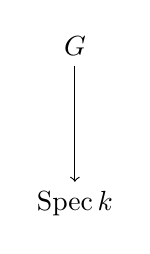
\begin{tikzpicture}
  \node (T) at (0, 2) {$G$};
  \node (B) at (0, 0) {$\Spec k$};
  \draw [->] (T) -- (B);
 \end{tikzpicture}
 \qquad\raisebox{.7in}{$k =$ perfect field of characteristic $p$} 
 \hskip -2.2in \raisebox{.4in}{$G =$ formal group of height $n$} 
\end{center}
and morphisms 
\begin{center}
 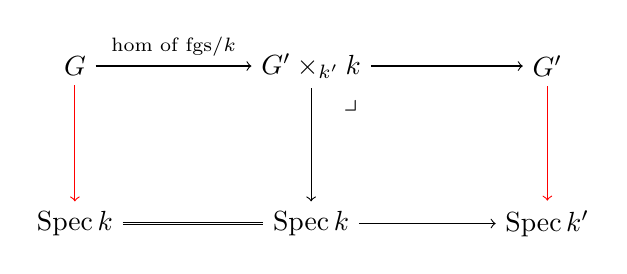
\begin{tikzpicture}
  \node (LT) at (0, 2) {$G$};
  \node (MT) at (3, 2) {$G' \times_{k'} k$};
  \node at (3.5, 1.5) {$\lrcorner$}; 
  \node (RT) at (6, 2) {$G'$};
  \node (LB) at (0, 0) {$\Spec k$};
  \node (MB) at (3, 0) {$\Spec k$};
  \node (RB) at (6, 0) {$\Spec k'$};
  \draw [->] (LT) -- node [above] {$\scriptstyle \text{hom of fgs$/k$}$} (MT);
  \draw [->] (MT) -- (RT);
  \draw [red,->] (LT) -- (LB);
  \draw [->] (MT) -- (MB);
  \draw [red,->] (RT) -- (RB);
  \draw [double] (LB) -- (MB);
  \draw [->] (MB) -- (RB);
 \end{tikzpicture}
\end{center}
(check: morphisms compose to morphism).  

Have also wide subcategories $\FG_\iso$ and $\FG_\isog$.  
Let $\FG(k)$ denote ``the usual thing.''  

\underline{Key example} 
\begin{center}
 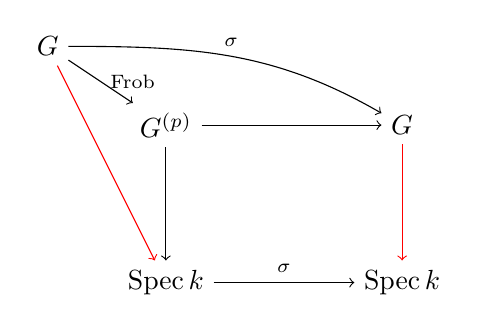
\begin{tikzpicture}
  \node (LT) at (1.5, 3) {$G$};
  \node (MT) at (3, 2) {$G^{(p)}$};
  \node (RT) at (6, 2) {$G$};
  \node (MB) at (3, 0) {$\Spec k$};
  \node (RB) at (6, 0) {$\Spec k$};
  \draw [->] (LT) -- node [right] {$\scriptstyle \Frob$} (MT);
  \draw [->] (LT) to [out = 0, in = 150]  node [above] {$\scriptstyle \sigma$} (RT);
  \draw [->] (MT) -- (RT);
  \draw [red,->] (LT) -- (MB);
  \draw [->] (MT) -- (MB);
  \draw [red,->] (RT) -- (RB);
  \draw [->] (MB) -- node [above] {$\scriptstyle \sigma$} (RB);
 \end{tikzpicture}
 \qquad\raisebox{1in}{$\sigma =$ absolute Frobenius} 
 \hskip -1.5in \raisebox{.4in}{endomorphism in $\FG_\isog$} 
 \hskip -1.55in \raisebox{.2in}{but {\em not} in $\FG_\isog(k)$} 
\end{center}
Denote this by $\Phi$.  
More generally, have 

\underline{Factorization in $\FG$} ~ Given 
\begin{center}
 \raisebox{.85in}{$\psi \co$} 
 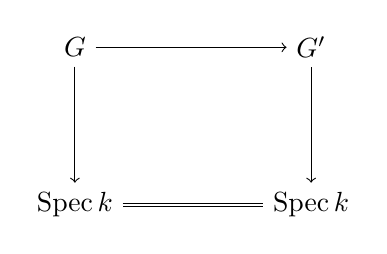
\begin{tikzpicture}
  \node (LT) at (0, 2) {$G$};
  \node (RT) at (3, 2) {$G'$};
  \node (LB) at (0, 0) {$\Spec k$};
  \node (RB) at (3, 0) {$\Spec k$};
  \draw [->] (LT) -- (RT);
  \draw [->] (LT) -- (LB);
  \draw [->] (RT) -- (RB);
  \draw [double] (LB) -- (RB);
 \end{tikzpicture}
 \raisebox{.85in}{in $\FG_\isog(k)$ of degree $p^r$} 
\end{center}
have a unique factorization of $\Phi^r$ (no ambiguity) with respect to $\psi$ as $\Phi^r = N_\psi \circ \psi$ 
\begin{center}
 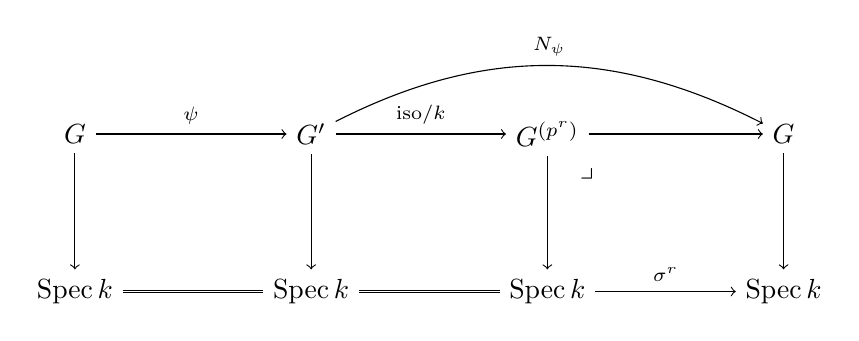
\begin{tikzpicture}
  \node (LT) at (0, 2) {$G$};
  \node (MLT) at (3, 2) {$G'$};
  \node (MRT) at (6, 2) {$G^{(p^r)}$};
  \node (RT) at (9, 2) {$G$};
  \node (LB) at (0, 0) {$\Spec k$};
  \node (MLB) at (3, 0) {$\Spec k$};
  \node (MRB) at (6, 0) {$\Spec k$};
  \node (RB) at (9, 0) {$\Spec k$};
  \draw [->] (LT) -- node [above] {$\scriptstyle \psi$} (MLT);
  \draw [->] (MLT) -- node [above] {$\scriptstyle {\rm iso} / k$} (MRT);
  \draw [->] (MRT) -- (RT);
  \draw [->] (LT) -- (LB);
  \draw [->] (MLT) -- (MLB);
  \draw [->] (MRT) -- (MRB);
  \draw [->] (RT) -- (RB);
  \draw [double] (LB) -- (MLB);
  \draw [double] (MLB) -- (MRB);
  \draw [->] (MRB) -- node [above] {$\scriptstyle \sigma^r$} (RB);
  \draw [->] (MLT) to [out = 27, in = 153] node [above] {$\scriptstyle N_\psi$} (RT);
  \node at (6.5, 1.5) {$\lrcorner$}; 
 \end{tikzpicture}
 \qquad\raisebox{.7in}{$N_\psi$ in $\FG_\iso$} 
\end{center}
On rings of functions, 
\begin{center}
 \hskip -1.1in
 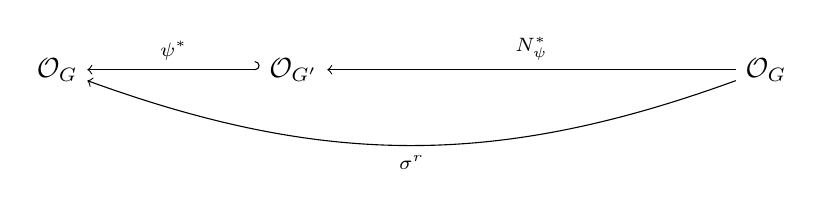
\begin{tikzpicture}
  \node (L) at (0, 0) {$\CO_G$};
  \node (ML) at (3, 0) {$\CO_{G'}$};
  \node (R) at (9, 0) {$\CO_G$};
  \draw [left hook->] (ML) -- node [above] {$\scriptstyle \psi^*$} (L);
  \draw [->] (R) -- node [above] {$\scriptstyle N_\psi^*$} (ML);
  \draw [->] (R) to [out = -160, in = -20] node [below] {$\scriptstyle \sigma^r$} (L);
 \end{tikzpicture}
\end{center}

\underline{Observation} 
\[
 N_\psi^* = {\rm Norm}({\CO_G}_{\CO_{G'}}^{\psi^*}) 
\]
the {\em norm} of $\CO_G$ as a finite free module over $\CO_G'$ along $\psi^*$.\footnote{Consider 
a coordinate on $G$ as a map $G \to \BA^1$ 
(an isomorphism of functors [Ando95, 2.1]).  
We have 
\[
 G \xrightarrow{\psi} G' \to \BA^1 
\]
and the above norm gives 
\[
 G \to \BA^1 \quad \mapsto \quad G' \to \BA^1 
\]
which is a {\em norm map} in the sense of equivariant stable homotopy theory ($G \to G/H \to R$ with $R$ a ring).  
}  

\underline{Example} ~ $\psi = \Frob$ 
\begin{center}
 \hskip -1.1in
 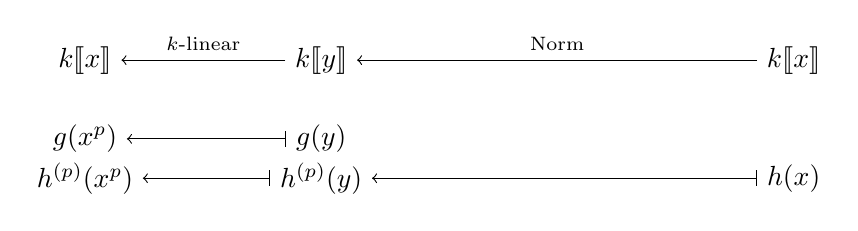
\begin{tikzpicture}
  \node (LT) at (0, 3) {$k\lb x\rb$};
  \node (MLT) at (3, 3) {$k\lb y\rb$};
  \node (RT) at (9, 3) {$k\lb x\rb$};
  \draw [->] (MLT) -- node [above] {$\scriptstyle \text{$k$-linear}$} (LT);
  \draw [->] (RT) -- node [above] {$\scriptstyle \text{Norm}$} (MLT);
  \node (LM) at (0, 2) {$g(x^p)$};
  \node (MLM) at (3, 2) {$g(y)$};
  \draw [|->] (MLM) -- (LM);
  \node (LB) at (0, 1.5) {$h^{(p)}(x^p)$};
  \node (MLB) at (3, 1.5) {$h^{(p)}(y)$};
  \node (RB) at (9, 1.5) {$h(x)$};
  \draw [|->] (MLB) -- (LB);
  \draw [|->] (RB) -- (MLB);
 \end{tikzpicture}
\end{center}
Norm can be directly calculated as follows.  
\begin{itemize}
 \item Multiplication by $x$ on $k\lb x\rb = \Span\{1,x,\ldots,x^{p-2},x^{p-1}\}$ over $k\lb y\rb$ 
 has determinant $(-1)^{1+p} y = y$.  

 \item Multiplication by $c \in k$ on $k\lb x\rb$ has determinant $c^p$.  

 \item The map is a ring homomorphism in characteristic $p$ (additive).  
\end{itemize}
Lifting the above, with $\psi = \Frob^n$ instead, we have (cf [email-3/31/16]) 
\[
 F/E_n \text{~lifts~} G/k 
\]
\begin{equation}
 \label{nm}
 \prod_{c \in F[p]} h\big(x +_F x(c)\big) = h^{(p^n)}\big(l_p(x)\big) \quad \text{for any $h \in E_n\lb x\rb$} 
\end{equation}
where $x$ is a ``norm-coherent'' lift of the coordinate on $G$, and $l_p$ lifts $\Frob^n/k$ (see below).  
Namely, the ``Lubin isogeny'' gives a formula for this norm [email-2/13/16],\footnote{As a homomorphism, 
the Lubin isogeny itself corresponds to the case $h(x) = x$.  
Compare the identity in [Coleman79, thm A], $\A_n = (\varphi^{-n} f_\A)(\upsilon_n)$, 
where the unique invertible formal Laurent series $f_\A$ 
seems to correspond to a change of coordinates from a given $y \sim \A$ to a norm-coherent $x = h^{-1}(y) \sim \upsilon$.  } 
because $F[p] = \Gal(\CO_F/\CO_{F'})$ 
with Galois action by adding a $p$-torsion point under the group law 
(cf Rotman, {\em Advanced modern algebra}, cor 10.87).  
It is invariant under $\Gal(\CO_F/\CO_{F'})$, and so in fact lies in $\CO_{F'}$.  
See [fkl', thm 4.9] and \href{https://youtu.be/r_7SsIoU9No?list=PLul8LCT3AJqQbjdfFSURcgoaik1EPJjc_}{its video} 
(before and after the break) for details and subtleties.  


\subsubsection{Pushforward deformation structures}

Given any isogeny $\psi \co F \to F/H= F'$ of degree $p^r$ 
and any deformation structure $(F,i,\eta)$ on the source, 
define the pushforward along $\psi$ 
\[
 (F,i,\eta) \stackrel{\psi_!}{\longmapsto} (F',i',\eta') 
\]
of deformation structures with respect to $G/k$ by 
\[
 i' = i \circ \sigma^r \co k \hookrightarrow R / {\mf m} 
\]
\[
 \eta' \circ \pi^*\psi = i^*\Frob^r \circ \eta 
\]
so that the following diagram commutes.  
\begin{center}
 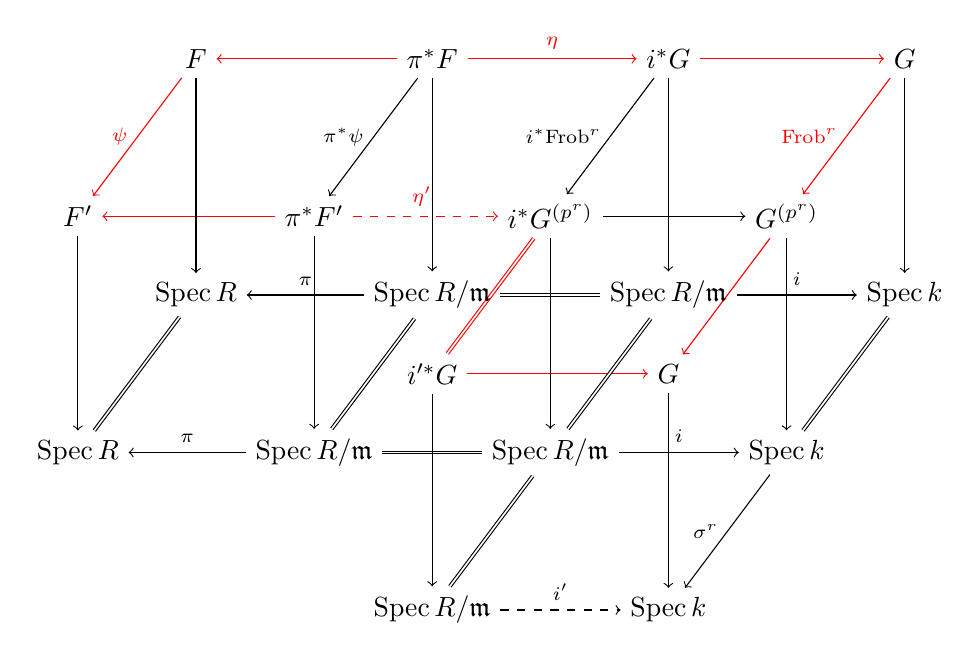
\begin{tikzpicture}
  \node (AA) at (3, 6) {$F$};
  \node (AB) at (6, 6) {$\pi^*F$};
  \node (AC) at (9, 6) {$i^*G$};
  \node (AD) at (12, 6) {$G$};
  \node (BA) at (1.5, 4) {$F'$};
  \node (BB) at (4.5, 4) {$\pi^*F'$};
  \node (BC) at (7.5, 4) {$i^*G^{(p^r)}$};
  \node (BD) at (10.5, 4) {$G^{(p^r)}$};
  \node (CC) at (6, 2) {$i'^*G$};
  \node (CD) at (9, 2) {$G$};
  \draw [red,->] (AB) -- (AA);
  \draw [red,->] (AB) -- node [above] {$\scriptstyle \eta$} (AC);
  \draw [red,->] (AC) -- (AD);
  \draw [->] (BC) -- (BD);
  \draw [red,->] (BB) -- (BA);
  \draw [red,dashed,->] (BB) -- node [above] {$\scriptstyle \!\! \eta'$} (BC);
  \draw [red,->] (CC) -- (CD);
  \draw [red,->] (AA) -- node [left] {$\scriptstyle \psi$} (BA);
  \draw [->] (AB) -- node [left] {$\scriptstyle \pi^*\psi$} (BB);
  \draw [->] (AC) -- node [left] {$\scriptstyle i^*\Frob^r$} (BC);
  \draw [red,double] (BC) -- (CC);
  \draw [red,->] (AD) -- node [left] {$\scriptstyle \Frob^r$} (BD);
  \draw [red,->] (BD) -- (CD);
  \node (AA') at (3, 3) {$\Spec R$};
  \node (AB') at (6, 3) {$\Spec R/{\mf m}$};
  \node (AC') at (9, 3) {$\Spec R/{\mf m}$};
  \node (AD') at (12, 3) {$\Spec k$};
  \node (BA') at (1.5, 1) {$\Spec R$};
  \node (BB') at (4.5, 1) {$\Spec R/{\mf m}$};
  \node (BC') at (7.5, 1) {$\Spec R/{\mf m}$};
  \node (BD') at (10.5, 1) {$\Spec k$};
  \node (CC') at (6, -1) {$\Spec R/{\mf m}$};
  \node (CD') at (9, -1) {$\Spec k$};
  \draw [->] (AB') -- node [above] {$\scriptstyle \pi$} (AA');
  \draw [double] (AB') -- (AC');
  \draw [->] (AC') -- node [above] {$\scriptstyle i$} (AD');
  \draw [->] (BC') -- node [above] {$\scriptstyle i$} (BD');
  \draw [->] (BB') -- node [above] {$\scriptstyle \pi$} (BA');
  \draw [double] (BB') -- (BC');
  \draw [dashed,->] (CC') -- node [above] {$\scriptstyle i'$} (CD');
  \draw [double] (AA') -- (BA');
  \draw [double] (AB') -- (BB');
  \draw [double] (AC') -- (BC');
  \draw [double] (BC') -- (CC');
  \draw [double] (AD') -- (BD');
  \draw [->] (BD') -- node [left] {$\scriptstyle \sigma^r$} (CD');
  \draw [->] (AA) -- (AA');
  \draw [->] (AB) -- (AB');
  \draw [->] (AC) -- (AC');
  \draw [->] (AD) -- (AD');
  \draw [->] (BC) -- (BC');
  \draw [->] (BD) -- (BD');
  \draw [->] (BA) -- (BA');
  \draw [->] (BB) -- (BB');
  \draw [->] (CC) -- (CC');
  \draw [->] (CD) -- (CD');
 \end{tikzpicture}
\end{center}
This lifts the endomorphism $\Phi^r \co G \to G$ in the wide category $\FG_\isog$ to $\Def_\isog(R)$.  

Question: Study $\Def$ (and similar examples) as a wide category equipped with pushforward [9/10/13].  


\subsubsection{Norm-coherent coordinates}

Given $G/k/\BF_p$ of height $n$, 
the subgroup of $p$-torsions $G[p] \subset G(\ck)$ is 
{\em stable} under $\Aut(\ck / k)$, in contrast to a subgroup of order $p^r$, $r<n$.  

Thus, given the universal deformation $F / E_n$ of $G / k$, 
and a coordinate $x$ on $F$ lifting a preferred coordinate on $G$, 
the Lubin isogeny 
\[
 f_p^x \co F_x \to F_x / F[p], 
\]
constructed with respect to $x$, can be defined over $E_n = A_0 \subset A_n$ 
(a generalization of [Lubin67, thm 1.4] to deformations).\footnote{Note that 
on the special fiber $\CO_{G^{(p^n)}} = k \lb y \rb$ over $k \stackrel{i}{=} E_n / {\mf m}$, 
this Lubin isogeny is $k$-linear, sending $g(y)$ to $g(x^{p^n})$.  
It is the relative $p^n$-power Frobenius 
and is {\em not} an endomorphism in general.  
In fact, by construction as a homomorphism of formal group {\em laws}, 
the Lubin isogeny determines a coordinate on $F/F[p]$ 
(see [Lubin67, thm 1.4] and cf [Ando95, prop 2.2.2]), lifting that on $G^{(p^n)}$.  }  

On the other hand, $l_p^x \co F_x \to \A_p^* F^{(p^n)}_x$ 
is characterized by the properties in [Ando95, prop 2.5.4], 
where $\A_p \co A_n \to E_n$ classfies the subgroup $F[p]$ of order $p^n$ 
(Strickland's theorem generalizing Lubin-Tate).\footnote{In particular, 
the condition (iii) there precisely means that, with respect to the deformation structure $(F,i,\eta)$, 
$k \otimes l_p^x$ is the relative Frobenius.  
\begin{center}
 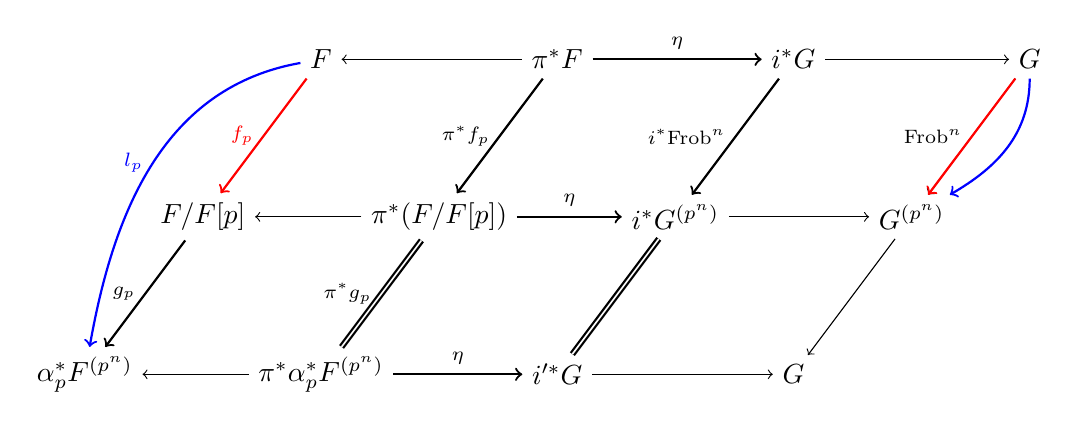
\begin{tikzpicture}
  \node (AA) at (3, 4) {$F$};
  \node (AB) at (6, 4) {$\pi^*F$};
  \node (AC) at (9, 4) {$i^*G$};
  \node (AD) at (12, 4) {$G$};
  \node (BA) at (1.5, 2) {$F/F[p]$};
  \node (BB) at (4.5, 2) {$\pi^*(F/F[p])$};
  \node (BC) at (7.5, 2) {$i^*G^{(p^n)}$};
  \node (BD) at (10.5, 2) {$G^{(p^n)}$};
  \node (CA) at (0, 0) {$\A_p^*F^{(p^n)}$};
  \node (CB) at (3, 0) {$\pi^*\A_p^*F^{(p^n)}$};
  \node (CC) at (6, 0) {$i'^*G$};
  \node (CD) at (9, 0) {$G$};
  \draw [->] (AB) -- (AA);
  \draw [thick,->] (AB) -- node [above] {$\scriptstyle \eta$} (AC);
  \draw [->] (AC) -- (AD);
  \draw [->] (BB) -- (BA);
  \draw [thick,->] (BB) -- node [above] {$\scriptstyle \eta$} (BC);
  \draw [->] (BC) -- (BD);
  \draw [->] (CB) -- (CA);
  \draw [thick,->] (CB) -- node [above] {$\scriptstyle \eta$} (CC);
  \draw [->] (CC) -- (CD);
  \draw [thick,red,->] (AA) -- node [left] {$\scriptstyle f_p$} (BA);
  \draw [thick,->] (AB) -- node [left] {$\scriptstyle \pi^*f_p$} (BB);
  \draw [thick,->] (AC) -- node [left] {$\scriptstyle i^*\Frob^n$} (BC);
  \draw [thick,blue,->] (AD) to [out = -90, in = 30] (BD);
  \draw [->] (AD) -- node [left] {$\scriptstyle \Frob^n$} (BD);
  \draw [thick,red,->] (AD) -- (BD);
  \draw [thick,->] (BA) -- node [left] {$\scriptstyle g_p$} (CA);
  \draw [thick,double] (BB) -- node [left] {$\scriptstyle \pi^*g_p$} (CB);
  \draw [thick,double] (BC) -- (CC);
  \draw [->] (BD) -- (CD);
  \draw [thick,blue,->] (AA) to [out = -170, in = 80] node [left] {$\scriptstyle l_p$} (CA);
\end{tikzpicture}
\\thick arrows are homomorphisms 
\end{center}
\vskip .7cm
For comparison, given any isogeny $\psi_H \co F \to F/H$ of degree $p^r$, we have 
\begin{center}
 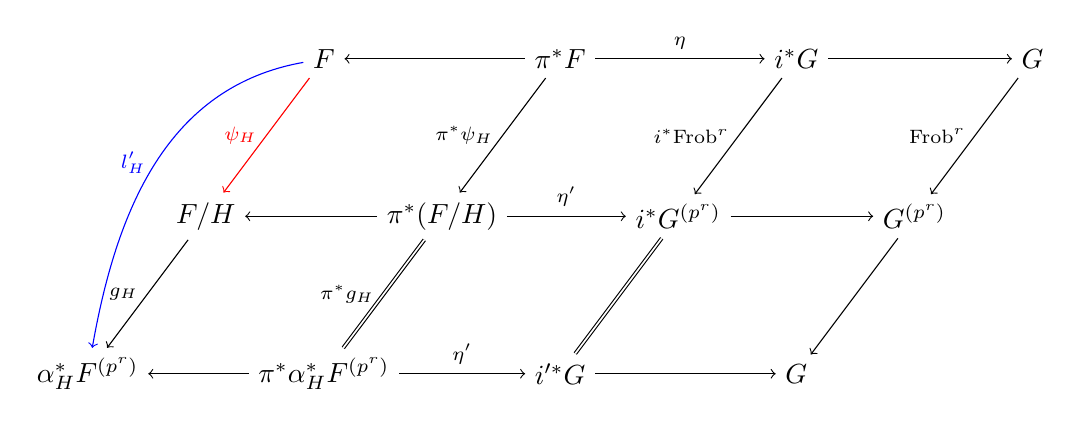
\begin{tikzpicture}
  \node (AA) at (3, 4) {$F$};
  \node (AB) at (6, 4) {$\pi^*F$};
  \node (AC) at (9, 4) {$i^*G$};
  \node (AD) at (12, 4) {$G$};
  \node (BA) at (1.5, 2) {$F/H$};
  \node (BB) at (4.5, 2) {$\pi^*(F/H)$};
  \node (BC) at (7.5, 2) {$i^*G^{(p^r)}$};
  \node (BD) at (10.5, 2) {$G^{(p^r)}$};
  \node (CA) at (0, 0) {$\A_H^*F^{(p^r)}$};
  \node (CB) at (3, 0) {$\pi^*\A_H^*F^{(p^r)}$};
  \node (CC) at (6, 0) {$i'^*G$};
  \node (CD) at (9, 0) {$G$};
  \draw [->] (AB) -- (AA);
  \draw [->] (AB) -- node [above] {$\scriptstyle \eta$} (AC);
  \draw [->] (AC) -- (AD);
  \draw [->] (BB) -- (BA);
  \draw [->] (BB) -- node [above] {$\scriptstyle \eta'$} (BC);
  \draw [->] (BC) -- (BD);
  \draw [->] (CB) -- (CA);
  \draw [->] (CB) -- node [above] {$\scriptstyle \eta'$} (CC);
  \draw [->] (CC) -- (CD);
  \draw [red,->] (AA) -- node [left] {$\scriptstyle \psi_H$} (BA);
  \draw [->] (AB) -- node [left] {$\scriptstyle \pi^*\psi_H$} (BB);
  \draw [->] (AC) -- node [left] {$\scriptstyle i^*\Frob^r$} (BC);
  \draw [->] (AD) -- node [left] {$\scriptstyle \Frob^r$} (BD);
  \draw [->] (BA) -- node [left] {$\scriptstyle g_H$} (CA);
  \draw [double] (BB) -- node [left] {$\scriptstyle \pi^*g_H$} (CB);
  \draw [double] (BC) -- (CC);
  \draw [->] (BD) -- (CD);
  \draw [blue,->] (AA) to [out = -170, in = 80] node [left] {$\scriptstyle l'_H$} (CA);
 \end{tikzpicture}
\end{center}
}  

This construction is functorial under base change and under quotient, 
due to the functorialities of Lubin's $f$ and of Strickland's $g$.  
Namely, there is a unique $\star$-isomorphism $g_p^x$ over $E_n$, and $l_p^x$ is {\em defined} as a composite 
\begin{center}
 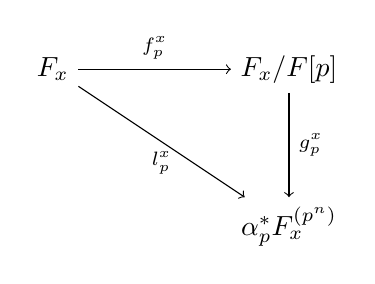
\begin{tikzpicture}
  \node (LT) at (0, 2) {$F_x$};
  \node (RT) at (3, 2) {$F_x / F[p]$};
  \node (RB) at (3, 0) {$\A_p^*F_x^{(p^n)}$};
  \draw [->] (LT) -- node [above] {$\scriptstyle f_p^x$} (RT);
  \draw [->] (LT) -- node [below] {$\scriptstyle l_p^x$} (RB);
  \draw [->] (RT) -- node [right] {$\scriptstyle g_p^x$} (RB);
 \end{tikzpicture}
\end{center}
The condition for $x$ to be {\em norm-coherent} is that 
\[
 f_p^x = l_p^x \hskip 1in \text{cf \eqref{nm} when $h(x) = x$} 
\]
that is, $g_p^x = \id$ (to be shown in construction of $x$).  

More generally, given a subgroup $H \subset F(A_r)$ of order $p^r$, 
on the special fiber, the Lubin isogeny $f_H^x$ equals $\Frob^r$, 
so the iso$/k$ in $N_f$ is $\id$ (with respect to this coordinate).  
\begin{center}
 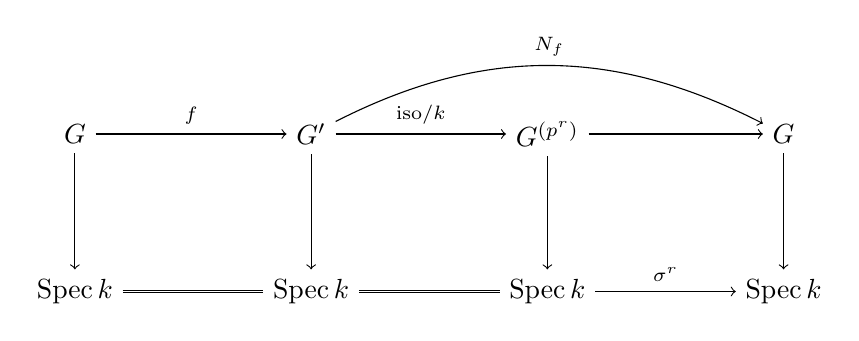
\begin{tikzpicture}
  \node (LT) at (0, 2) {$G$};
  \node (MLT) at (3, 2) {$G'$};
  \node (MRT) at (6, 2) {$G^{(p^r)}$};
  \node (RT) at (9, 2) {$G$};
  \node (LB) at (0, 0) {$\Spec k$};
  \node (MLB) at (3, 0) {$\Spec k$};
  \node (MRB) at (6, 0) {$\Spec k$};
  \node (RB) at (9, 0) {$\Spec k$};
  \draw [->] (LT) -- node [above] {$\scriptstyle f$} (MLT);
  \draw [->] (MLT) -- node [above] {$\scriptstyle {\rm iso} / k$} (MRT);
  \draw [->] (MRT) -- (RT);
  \draw [->] (LT) -- (LB);
  \draw [->] (MLT) -- (MLB);
  \draw [->] (MRT) -- (MRB);
  \draw [->] (RT) -- (RB);
  \draw [double] (LB) -- (MLB);
  \draw [double] (MLB) -- (MRB);
  \draw [->] (MRB) -- node [above] {$\scriptstyle \sigma^r$} (RB);
  \draw [->] (MLT) to [out = 27, in = 153] node [above] {$\scriptstyle N_f$} (RT);
 \end{tikzpicture}
 \qquad\raisebox{.7in}{$N_f$ in $\FG_\iso$} 
\end{center}

This iso$/k$ lifts to an iso $g_H$ over $A_r$ (coordinatewise $g_H^x$ is a $\star$-iso) 
and we get a diagram of formal group laws 
\begin{center}
 \hskip -2.27in
 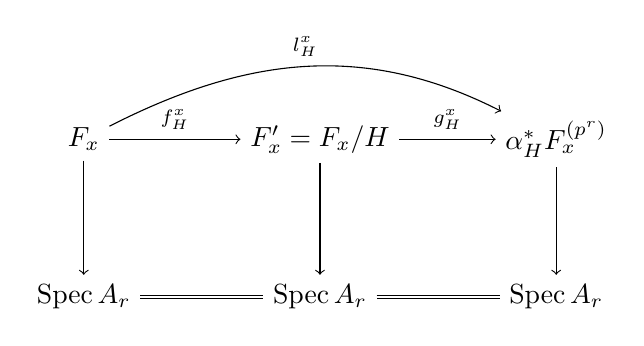
\begin{tikzpicture}
  \node (LT) at (0, 2) {$F_x$};
  \node (MT) at (3, 2) {$F_x' = F_x / H$};
  \node (RT) at (6, 2) {$\A_H^* F^{(p^r)}_x$};
  \node (LB) at (0, 0) {$\Spec A_r$};
  \node (MB) at (3, 0) {$\Spec A_r$};
  \node (RB) at (6, 0) {$\Spec A_r$};
  \draw [->] (LT) -- node [above] {$\scriptstyle f_H^x$} (MT);
  \draw [->] (MT) -- node [above] {$\scriptstyle g_H^x$} (RT);
  \draw [->] (LT) -- (LB);
  \draw [->] (MT) -- (MB);
  \draw [->] (RT) -- (RB);
  \draw [double] (LB) -- (MB);
  \draw [double] (MB) -- (RB);
  \draw [->] (LT) to [out = 27, in = 153] node [above] {$\scriptstyle l_H^x$} (RT);
 \end{tikzpicture}
\end{center}
A norm-coherent coordinate $x$ is such that $g_H^x = \id$, 
for any $H \subset F$.  
In other words, 
\[
 l_H^x = f_H^x 
\]
which, as a universal example ($\eta' = \eta$), expresses the fact that 
\begin{equation}
 \label{pushnorm}
 x_{F', \psi_! d} = N_\psi^* (x_{F,d}) 
\end{equation}
along {\em any} isogeny $\psi \co F \to F'$ with any deformation structure $d$ [email-2/13/16].  
Cf [fkl', thm 4.9] and [AHS04, prop 4.13].  


\subsubsection{Ando's construction of norm-coherent coordinates in greater generality}

The proof of [Ando95, thm 2.5.7] combines two theorems.  
Replace $[p] \co F \to F$ by $l_p \co F \to \A_p^* F^{(p^n)}$, both over $E_n$, in the following.  
\begin{enumerate}[(i)]
 \item Thm 2.6.4 (the $p$-torsion subgroup) 

 Want a coordinate $x$ on $F$ (lifting a preferred coordinate on $G/k/\BF_p$) that satisfies 
 \begin{equation}
  \label{nmcoh}
  \hskip 6cm f_p^x = l_p^x \hskip 2cm \text{norm-coherence for $H = F[p]$} 
 \end{equation}
 \begin{itemize}
  \item Existence 
  \begin{itemize}
   \item [$\circ$] Reduction to the universal case: replace 2.6.5 by showing 
   \[
    l_{_p\B_*G}^{\B_*x} = \B_* l_{_pG}^x 
   \]
   This is the functoriality of $l_H^x$ under base change.  

   \item [$\circ$] Construction of a norm-coherent coordinate on $F_\univ$ 

   Replace 2.6.7 by showing that 
   \begin{center}
    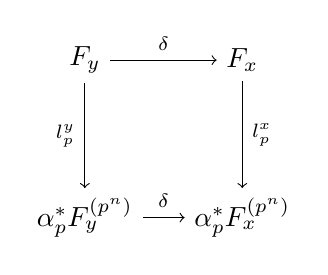
\begin{tikzpicture}
     \node (LT) at (0, 2) {$F_y$};
     \node (RT) at (2, 2) {$F_x$};
     \node (LB) at (0, 0) {$\A_p^*F_y^{(p^n)}$};
     \node (RB) at (2, 0) {$\A_p^*F_x^{(p^n)}$};
     \draw [->] (LT) -- node [above] {$\scriptstyle \d$} (RT);
     \draw [->] (LB) -- node [above] {$\scriptstyle \d$} (RB);
     \draw [->] (LT) -- node [left] {$\scriptstyle l_p^y$} (LB);
     \draw [->] (RT) -- node [right] {$\scriptstyle l_p^x$} (RB);
    \end{tikzpicture}
   \end{center}
   commutes: $\d$ is a $\star$-isomorphism,\footnote{The lower $\d$ is an abuse of notation.  } 
   and thus $\d \circ l_p^y \circ \d^{-1} = l_p^x$ by uniqueness in 2.5.4.  
   This is the functoriality of $l_H^x$ under quotient (by the trivial subgroup).  

   The rest carries through.  

   Note: the special property of $H = F[p]$ used in the proof is that 
   $g_p$ is defined over $E_n$ and hence $\d$ is a change of coordinates on $F$.  
  \end{itemize}

  \item Uniqueness 

  Also needs the above functoriality of $l_H^x$ under base change to apply to general $F$.  
 \end{itemize}

 \item Prop 2.6.15 (all subgroups) 

 Given any $H \subset F[p^k](A_r)$ of order $p^r$ (with $k \geq r$), 
 show that the $\star$-isomorphism 
 \[
  F_x/H \xrightarrow{g_H^x} \A_H^* F^{(p^r)}_x 
 \]
 is the identity by the above uniqueness.  
 \begin{itemize}
  \item Target satisfies \eqref{nmcoh} 

  Follows from the reduction to the universal case above.  
  Note that $F^{(p^r)}$ {\em is} a deformation of $G/k$ with structure $(i' = i \circ \sigma^r, \eta')$.  

  \item Source satisfies \eqref{nmcoh} 

  Replace 2.6.16 by 
  \begin{center}
   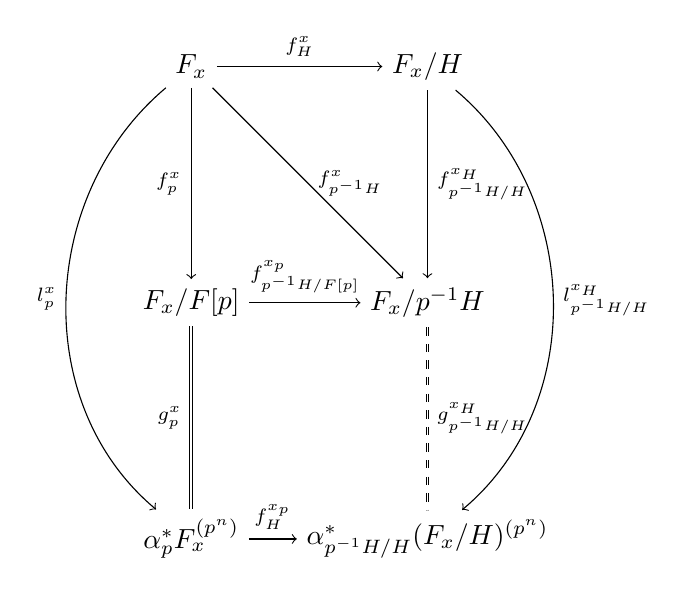
\begin{tikzpicture}
    \node (LT) at (0, 6) {$F_x$};
    \node (RT) at (3, 6) {$F_x/H$};
    \node (LM) at (0, 3) {$F_x/F[p]$};
    \node (RM) at (3, 3) {$F_x/p^{-1}H$};
    \node (LB) at (0, 0) {$\A_p^*F_x^{(p^n)}$};
    \node (RB) at (3, 0) {$\A_{p^{-1}H/H}^*(F_x/H)^{(p^n)}$};
    \draw [->] (LT) -- node [above] {$\scriptstyle f_H^x$} (RT);
    \draw [->] (LB) -- node [above] {$\scriptstyle f_H^{x_p}$} (RB);
    \draw [->] (LM) -- node [above] {$\scriptstyle f_{p^{-1}H/F[p]}^{x_p}$} (RM);
    \draw [->] (LT) -- node [left] {$\scriptstyle f_p^x$} (LM);
    \draw [double] (LM) -- node [left] {$\scriptstyle g_p^x$} (LB);
    \draw [->] (RT) -- node [right] {$\scriptstyle f_{p^{-1}H/H}^{x_H}$} (RM);
    \draw [->] (LT) -- node [right] {$\scriptstyle f_{p^{-1}H}^x$} (RM);
    \draw [dashed,double] (RM) -- node [right] {$\scriptstyle g_{p^{-1}H/H}^{x_H}$} (RB);
    \draw [->] (LT) to [out = -140, in = 140] node [left] {$\scriptstyle l_p^x$} (LB);
    \draw [->] (RT) to [out = -40, in = 40] node [right] {$\scriptstyle l_{p^{-1}H/H}^{x_H}$} (RB);
   \end{tikzpicture}
  \end{center}
  same idea though, using 2.2.6 crucially (note that in the lower square $H = p^{-1}H/F[p]$).  
  More generally, this is the functoriality of $l_K^x$ under quotient.  
 \end{itemize}
\end{enumerate}

\underline{Functoriality} [email-2/14/16, email-4/14/16] 

Let $\Ando\co\FG_\isog\to\Set$ be the bivariant functor 
\[
 G/k \mapsto \{\text{norm-coherent coordinates on $F/E_n$}\} 
\]
that respects pullback and base change contravariantly and pushforward covariantly.  

Let $\Coord\co\FG_\isog\to\Set$ be the bivariant functor 
\[
 G/k \mapsto \{\text{coordinates on $G$}\} \subset \CO_G 
\]

\begin{thm}
 The natural transformation 
 \[
  \Ando\to\Coord 
 \]
 of restriction to the special fiber is an isomorphism.  
 Moreover, it respects Galois descent: given a Galois extension $K/k$, the following diagram commutes.  
 \begin{center}
  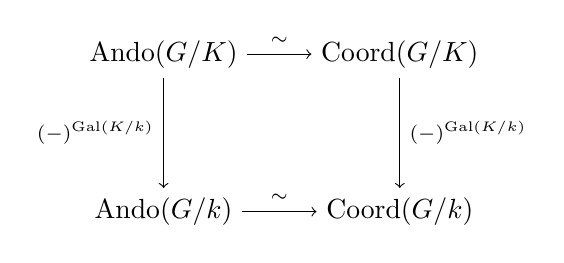
\begin{tikzpicture}
   \node (LT) at (0, 2) {$\Ando(G/K)$};
   \node (RT) at (3, 2) {$\Coord(G/K)$};
   \node (LB) at (0, 0) {$\Ando(G/k)$};
   \node (RB) at (3, 0) {$\Coord(G/k)$};
   \draw [->] (LT) -- node [above] {$\scriptstyle \sim$} (RT);
   \draw [->] (LB) -- node [above] {$\scriptstyle \sim$} (RB);
   \draw [->] (LT) -- node [left] {$\scriptstyle (-)^{\Gal(K/k)}$} (LB);
   \draw [->] (RT) -- node [right] {$\scriptstyle (-)^{\Gal(K/k)}$} (RB);
  \end{tikzpicture}
 \end{center}
\end{thm}

\underline{$H_\infty$ complex orientations for Morava $E$-theories} 

[AHS04, prop 6.1] with $k = 0 \leftrightsquigarrow$ \eqref{pushnorm}.  
Cf [FPFP, \S 29].  

Question: Can these be made $E_\infty$?  
Cf [Walker] and [M\"oller].  
Obstructions at higher height?  

$H_\infty$ maps are the
elements on the zero line of some spectral sequence for getting $E_\infty$
maps, and the higher terms on the spectral sequence have something to do
with Andre-Quillen cohomology and might be relatively easy to compute.


\newpage
\section{Move on}

\subsection{Application to computation with tmf with level structure}

$E = L_{K(2)} \TMF(\G_1(4))$ at $p = 3$ 

Xu 


\subsection{Study power operations in related cohomology theories}
\label{subsec:relct}

quasi-elliptic cohomology (interpolate with height 1, cusps), Huan [email, 4/17/13], Rezk, Ganter 

equivariant elliptic cohomology 


\subsection{Reduction mod p}

\textbf{[mc1]}, [email, 7/27/11], Section \ref{subsec:Qmodp}, cf [KM, 13] 

The Igusa tower [Bnotes] 


\subsection{Revisit [h2p2, esp 2] and [slides], and extensions}

[h2] 

other operations and operators associated to $E$ at h2p3: 
$\theta$, $\Psi$ (Adem relations), trace and norm (commutation relations), logarithm in [h2p2]; [ando92], [ganter06], [log] (Clausen) 

Koszul 


\subsection{$K(1)$-local applications}

[Section \ref{sec:level3}] 
calculations (abundance of different forms under the rug): 
existence of a generalized $BP\langle2\rangle$ at the prime 3 as an $E_\infty$-ring spectrum 

functoriality / geometric interpretation of closure under operations (something analogous to our approach to Adem relations??) 
[level3', p6]: crystalline Dieudonn\'e theory, a rank 2 $F$-crystal over $\BZ_p \llbracket a \rrbracket$ with specific rationality properties 

connection to power operations in quasi-elliptic cohomology [email, 4/17/13] 

[$K(1)E_\infty$]: explicit $K(1)$-local power operation formulas might help? revisit [hopkins] (see sec \ref{subsec:h2p2}) 


\subsection{Functoriality}
\label{subsec:fcr}

a better model for the power operation structure 


\subsection{Study the ``dual'' \DL algebra and related structures}

Milnor-Moore '65, how to generalize to {\em twisted} bialgebras?  ``connected'' 

Milnor '58 


\subsection{Experiments}
\label{subsec:exp}

\begin{itemize}
 \item $[\G_1(5), \omega]$ ([ormsby, behrensormsby]) at $p=2$ 

 \item {[Legendre]} ([K2S, 1.3.2]) at $p=3$ (Nendorf?) 

 \item $[\G_1(3), \omega]$ ([tmf3, 3.2]) at $p=5$ ($p-1 \nmid h$ [Wed-4/3/13]) 

 \item $[\G_1(4), \omega]$ at $p=5$ 
\end{itemize}

parameters: [KM, 7.7-8], [ando95, 2.5.7] 

algorithmic aspects: ``V\'elu's formulas'' for the Lubin isogeny in $uv$-coordinates, 
computer packges in Sage for calculations with elliptic curves and the Steenrod algebra 


\subsection{Thu-2/21/13}


\subsection{Tue-3/5/13}

McClure, $K(1)$-homology of $QX$ 

Calculate, using power operations, $K(2)$-homology of $QX$.  (Kashiwabara?) 


\subsection{Tue-3/19/13}


\subsection{Tue-9/10/13}

Global theory: [survey], [QuasiEll], [global], [email, 9/21/13] 
in connection with Sections \ref{subsec:relct}, \ref{subsec:fcr} (functoriality -> local-to-global) and \ref{subsec:exp} (recollement) 

\end{document}